\documentclass[11pt,makeidx,english]{style/phdthesis}
\usepackage[english]{babel}

\usepackage{amsmath}
\usepackage{amsopn}
\usepackage{amsthm}
\usepackage[floatperchapter]{classicthesis}

\usepackage[utf8]{inputenc}
\usepackage[T1]{fontenc}

\usepackage{url}
\usepackage{natbib}
\usepackage{bibentry}
\usepackage{supertabular}
\usepackage{tabularx}
\usepackage{latexsym}
\usepackage{graphicx}
\usepackage{placeins}
\usepackage{framed}
\usepackage{pbox}
\usepackage{tikz}
\usepackage{pgfplots}
\usepackage{microtype}
%\usepackage{FiraMono}
\usepackage{listings}
\usepackage{covington}
\usepackage[super]{nth}
\usepackage{titlesec}
\usepackage[font={it}]{caption}
\usepackage{algorithm}
\usepackage{algpseudocode}
\usepackage{gb4e} %this conflicts with underscores in filenames for some obscure reason!!! take care not to use underscores!
\usepackage{chngcntr}
\counterwithout{footnote}{chapter}
\usepackage{titletoc}
\titleclass{\part}{top}
\titleformat{\part}[display]
  {\normalfont\Huge}{\centering\thepart}{1em}{\centering}%
  [\setcounter{chapter}{0}]% <- added to reset the chapter counter for each part

\contentsmargin{0pt}%<- added (as suggested by jvd in a comment)

\titlecontents{part}[10mm]% <- changed
  {\vspace{12pt}\large\normalfont\bfseries}
  {\contentslabel{10mm}}{}
  {\hfill\thecontentspage}

\titlecontents{chapter}[10mm]
  {\vspace{4pt}\normalsize\normalfont\bfseries}
  {\contentslabel{10mm}}{}
  {\hfill\thecontentspage}

\titlecontents{section}[22.3mm]
  {\vspace{0pt}\normalsize\normalfont}
  {\contentslabel[\thecontentslabel]{12.3mm}}{}
  {\titlerule*[.75em]{.}\thecontentspage}

\titlecontents{subsection}[28.3mm]
  {\vspace{0pt}\normalsize\normalfont}
  {\contentslabel[\thecontentslabel]{12.3mm}}{}
  {\titlerule*[.75em]{.}\thecontentspage}

\usepackage{footnote}
\makesavenoteenv{tabular}
\makesavenoteenv{table}
%\usepackage{scrextend}
\let\proof\relax
\let\endproof\relax
\newtheoremstyle{break}
  {\topsep}{\topsep}%
  {\itshape}{}%
  {\bfseries}{}%
  {\newline}{}%
\theoremstyle{break}
\newtheorem{exmp}{Example}[section]
\DisableLigatures{encoding = *, family = tt*}

\DeclareMathOperator*{\argmin}{arg\,min}
\DeclareMathOperator*{\argmax}{arg\,max}

\pgfplotsset{compat=newest}
%\usetikzlibrary{external}
%\usepgfplotslibrary{external}
%\tikzexternalize

% customize section
\titleformat{\section}%
{\Large\bfseries}% format
{\llap{% label
    \thesection\hskip 9pt}}%
{0pt}% horizontal sep
{}% before

% customize subsection
\titleformat{\subsection}%
{\bfseries}% format
{\llap{% label
    \thesubsection\hskip 9pt}}%
{0pt}% horizontal sep
{}% before



%\thesistitle{Context as Linguistic Bridges}
%\supervisor{Antal van den Bosch}
%\degree{Doctor of Philosophy}
\author{Maarten van Gompel}

%\university{Radboud University Nijmegen}

\begin{document}

\frontmatter

\pagestyle{plain}



\begin{titlepage}
\begin{center}
\vspace{8cm}
{\Huge Context as Linguistic Bridges}


\vspace{1cm}
Een wetenschappelijke proeve op het gebied van de Letteren

\vspace{6cm}
{\LARGE Proefschrift }\\
\vspace{1cm}
ter verkrijging van de graad van doctor\\
aan de Radboud Universiteit Nijmegen\\
op gezag van de rector magnificus prof. dr. J.H.J.M van Krieken,\\
volgens besluit van het college van decanen.\\

\vspace{2cm}

door\\
\vspace{1cm}
{\LARGE Maarten van Gompel}\\
\vspace{0.5cm}
geboren op 15 december 1982\\
te Etten-Leur


\vspace{0.5cm}


\end{center}

\clearpage

\thispagestyle{empty}
\begin{tabular}{ll}
Promotoren: & Prof. dr. A. van den Bosch \\
 & \\
Manuscriptcommissie: & \\
\end{tabular}
prof. dr. L.A.L. van de Wijngaert (Voorzitter)  \\
prof. dr. L. Macken (Universiteit Gent, België) \\
prof. dr. P.T.J.M. Vossen (Vrije Universiteit Amsterdam) \\
prof. dr. E.J. Krahmer  (Tilburg University) \\
dr. C. Monz  (Universiteit van Amsterdam) \\
\end{titlepage}



\includegraphics[width=2.0cm]{siks.zw.png} \\
SIKS Dissertation Series No. 2020-04 \\
The research reported in this thesis has been carried out under the auspices of SIKS, the Dutch Research School for
Information and Knowledge Systems.

\textsuperscript{\textcopyright} 2020 Maarten van Gompel \\
\emph{This work is licensed under a Creative Commons Attribution-ShareAlike 4.0 International License:
\url{https://creativecommons.org/licenses/by-sa/4.0/}.} \\
Sources: \url{https://github.com/proycon/phd-thesis}. \\

Cover drawing (hummingbird) by \emph{Elke van Gompel}, all rights reserved. \\
Written in (neo)vim on Arch Linux, typeset in \LaTeX \\

\chapter*{Acknowledgements}
\addcontentsline{toc}{chapter}{Acknowledgements}
\markboth{Acknowledgements}{Acknowledgements}

Thanks first and foremost goes to Antal van den Bosch, with whom I moved from
Tilburg University to Radboud University to start this PhD research and who has
been my supervisor throughout, as well as co-author of many papers. Together we formed
the ideas and intuitions that drove this research, adjusting our direction as
we went along. Our research together already started in 2009
and culminated in my Master's thesis at that time.

Two years later, just after summer 2011, we stood at the dawn of the
development of a new research group in Nijmegen that would later come to be
known as the ``Language Machines'', or affectionately called ``the lamas''.  I
am happy to have been present since its inception, and happy to see
various familiar faces from our previous research group join us, as well as
meet many new colleagues who joined us. On the flip side, I am sad to see various colleagues
move on and the group shrinking considerably these past few years, but such is life.

I am immensely grateful for the confidence and freedom I received throughout the
years, also from Henk van den Heuvel of the Centre of Language and Speech
Technology (CLST), to work primarily from home and forego on any far travels,
which my health situation prohibits unfortunately. I have had the opportunity to take
initiative in starting numerous research software development projects. Many of
those go under the umbrella of CLARIN-NL and later CLARIAH; to name a few:
CLAM, FoLiA, FLAT, LaMachine, Ucto... In the light of the combined weight of
all this research software, I even consider the current work that lies before
you relatively minor, notwithstanding the effort that has gone into it and the
great opportunity it has been.

I want to thank the co-authors of Chapter~\ref{chap:semeval2014task5}, Iris
Hendrickx and Els Lefever, without whom the shared task for SemEval that we
describe in that chapter would not have been possible. Similarly, thanks also
goes to the participants in that shared task. I consider this line of
investigation one of the more succesful outcomes of this PhD project.

Finishing the dissertation was not without its challenges. The research itself
had already finished in early 2016 but it was apparent that it became largely a
negative result report rather than the breakthrough one initially hopes for.
This was also cause for some rejections from publishers, regarding
Chapters~\ref{chap:colibritafinal} and \ref{chap:sourcecontextinsmt}. In the
meantime the various other research software development projects proved quite
succesful and took up so much time that there was little time, and less
motivation, left to actually finish the dissertation. Thanks to CLST funding I
was eventually able to take some time to stop other activities and direct
all focus to completion of the dissertation and its defense.

Thanks to my sister Elke for drawing the beautiful hummingbird that you see on the cover of this book.  We have a bit of
a tradition to name our software after animals, so I wanted to continue in this tradition for the software that sprung
from this research (see Chapters~\ref{chap:coco} and \ref{chap:colibritafinal}), as well as for the project as a whole.
Colibri, or some variation thereof, is the word for hummingbird in many languages, and is an acronym of the somewhat
cryptic title of this dissertation: \emph{Constructions as Linguistic Bridges}.

Last, but certainly not least, thanks goes to my boyfriend Hans for his endless patience in putting up with
me (and no less important; feeding me!) when I often work strange hours and zone
out as I am emerged in some work-related project, whether it is programming or
writing this dissertation, or even chatting with colleagues on our IRC chat.
The latter has proven a most cherished tool that allows me to keep in touch
with my colleagues no matter the time or place!



\tableofcontents

%weggelaten, niet nuttig
%\listoffigures
%\listoftables

%\include{frontmatter}

\mainmatter
\pagestyle{headings}


\chapter{Introduction}

“To know an object is to lead to it through a context which the world
provides.” -- William James (American Philospher, 1861-1947)

"Form is emptiness, emptiness is form" -- Heart Sutra

\section{Context as Linguistic Bridges}

\subsection{Context}

To even begin to merit the title of ``Doctor of Philosophy'', it is only proper
to start this dissertation with some philosophical deliberations. This will be
in sharp contrast to more technical nature of the rest of these chapters.

The study you are about to read sprung from the intuition that \emph{context}
is an important, if not the most important, characteristic that defines
language. Language itself only exists only in the context of the world that
surrounds us, as well our internal mental world. Without this context, there is
nothing to talk about in the first place. Language is rightfully considered the
epitome of human evolution. Our species evolved the remarkable ability to refer to the
world outside and within by producing complex meaningful utterances, i.e. speech. 

This was an unparalleled revolution in \emph{communication}, which has
undoubtedly played a leading role in us becoming the dominant intelligent species
on the planet. It has put us in a position where we can communicate our
thoughts and feelings about the world to one another on a more fine-grained
level than any other species can. Moreover, it has given us the ability of ever increasing
\emph{abstraction}. The context of our language is no longer limited to just
refer to objects in our immediate vicinity, but we can even refer to abstract
thought itself. Whenever communication is attempted between people who do not
share a language, the context to which can be referred is dramatically restricted.
Just imagine tourists in a foreign bakery lustfully pointing at the
pastries they desire. 

Another major revolution in communication has been the development of writing,
and much later that of print technology. This and the accompanied literacy of
populations allows for our thoughts and ideas to be preserved more easily and
accurately than oral traditions can accomplish. The ability to read and write
broadens one's world, one's context, and is therefore even deemed a fundamental
human right. 

Language is inherently ambiguous and context is the disambiguating factor
without which it can not exist. The context of a bakery and a neatly arranged
line of pastries is essential for the baker to be able to disambiguate the
pointing of the clueless foreign tourist and discern which pastry he actually
wants. Demonstrative pronouns such as ``he'', ``she'', ``this'', or even
definite noun phrases such as ``the house'' convey little information if not
for the context they're employed in.  In fact, any word by itself is pretty
limited, can never exist in total isolation, and only derives meaning from the
further context. It is even defined purely through the context, just like a
dictionary defines words in terms of other words.

Buddhist philosophy has a concept called शून्यता. Sorry? You couldn't decipher
these cute curly snakes hanging from a line? If the context of your own
upbringing was Indian and you had been brought up learning how to read
devanagari script, you would probably be able to read that as ``shunyata''.
Merely being able to read and vocalize the word still wouldn't bring you closer
to its meaning though. The word is Sanskrit, though it comes from a Pali word,
as is the form in which it is written in an Buddhist scripture called the
``Heart Sutra''. 

The fact we can can even still talk about this word and its usage in a
2500-year old text today is already a testimony to the major impact writing
technology has on our civilization. Hundreds of millions of adherents of
various major religions still derive their daily religious practice from
throughts and ideas put down in writing in ancient times. Moreover, as a
scientific community, we base our studies on the work of our predecessors,
explicitly citing them as our methodology requires. But I digress, as my
main point relates to the meaning of sunyata. 

Sunyata can be translated into English as ``emptiness'' and refers to the idea
that everything, not just words, is interrelated and nothing has any existence
or essence of or by itself: this philosophy posits that everything exists and
is defined purely through \emph{its context}.

\subsection{Linguistic Bridges}

Whereas we humans all share an astounding capacity for language, history has
given rise to numerous distinct and often mutually unintelligable languages.
This bring us back to the predicament of our pastry-loving tourist in the
foreign bakery, unable to express his choice in the language of the baker and
therefore resorting to pointing. If we situate the bakery in France, the baker
may reply ``croissant'' in response to the gesturing of his client. The
perceptive client may then have learned that this is what the pastry is called.
The famous utterance ``Me Tarzan, You Jane'', heavily supported by gestures as in
the classic movie ``The Ape Man'', is of a similar nature. Both protagonists
breach the language barrier and gain new information. These example show that context
plays an important role in establishing translation, or any common vocabulary. 

The \emph{linguistic bridges} of this dissertation refer to these acts of
translation. We can define translation as \emph{a process that yields a
representation of a message initially expressed in one language, in another}.
Etymologically, the word \emph{translation}, from the latin \emph{translātiō},
refers to carrying (lātiō) accross (trans) something. The focus is generally on
accurate preservation of the semantics of message.  Although in some arts, such
as poetry, form or emotion may take presendence over the substance.

The intuition underlying our research is that the context of word or phrase is
an important cue for the translation of that word or phrase. A word in context
A, may be translated differently than the same word in context B. Consider the
Portuguese word ``tempo`` in the following sentences:

\begin{enumerate}
\item ``O \textbf{tempo} é bom hoje.'' -- ``The \textbf{weather} is nice today.''
\item ``Não tenho \textbf{tempo} para estudar hoje.'' -- ``I don't have \textbf{time} to study today.''
\end{enumerate}

In the first sentence, ``tempo`` is translated as ``weather'', whereas in the
second it is translated as ``time''. Portuguese uses the same word where
English uses two distinct words; context provides cues to disambiguate into the
proper translation. Another example shows where English has one word and French has two:

\begin{enumerate}
\item ``J'ai tué \textbf{la mouche}'' -- ``I killed \textbf{the fly}''
\item ``Je \textbf{vole} à Paris'' - ``I \textbf{fly} to Paris''
\item ``Je \textbf{vole} l'horloge de mon père'' -- ``I steal my father's watch''
\end{enumerate}

In this latter example, disambiguation between the first two sentences is
facilitated by the fact that the word \emph{fly} has a different
part-of-speech in both sentences, unlike the noun \emph{tempo} in the earlier example.
The presence of the article ``the'' in the noun phrase ``the fly'' already
rules out a translation to a verb. The French verb ``voler'' in turn does not
just translate to ``to fly'', but can also mean ``to steal'', as shown in
the last sentence. 

These examples illustrate that languages are almost never translatable on a naive
word-by-word basis, and that context plays an major role in determining the
right translation. Context plays a bridging function in translation, and this
dissertation investigates techniques for machines to exploit this to attain
better automatic translations.

\subsection{Natural Language Processing}

In our philosophical deliberations we briefly addressed the communication
revolutions brought about by humanity evolving the faculty of language and
speech, and later the technological development of writing and print. We all
live in fortunate times to have just witnessed the biggest revolution in
communication since the invention of print: the information revolution. Text is
not just printed anymore, it is digitized; i.e. made available, distributable,
and searchable in digital form. The internet enables these digital resources to
be collected, shared, and exploited at unpredecented rate and allows us to
communicate instantaneously with people from all over the planet. 

To emphasize the importance of this development, and to underline my personal
conviction that this is the way the future should go; this dissertation itself will
be made available primarily in an open digital form, rather than printed book form.

This wealth of digitized data fuels our field of research: Natural Language
Processing (NLP). We attempt to extract meaningful data from natural language.
Most contemporary techniques in NLP are grounded in Machine Learning, which
employs statistical principles to learn whatever patterns from big collections
of natural language data. These data-driven approaches in NLP can be contrasted to
the more rule-based approaches, not without their own merit, that are directly
derived from human expert knowledge.

This dissertation strictly follows the data-driven trend and we therefore rely
on large amounts of digitized text to conduct our research.


%%

\subsection{}

To investigate the role of context information in translation, our
begins in a field that shares a 






\subsection{Machine Translation}

The area of research dedicated to the automatic translation of data from one
natural language to another is called \emph{Machine Translation} (MT).
State-of-the-art techniques in this field are primarily based on statistical
methods, in which case we can speak of \emph{Statistical Machine Translation}
(SMT). 

Early methods in Machine Translation 



\section{Thesis structure}

























%Copyright Notice
%Authors who publish with this journal agree to the following terms:

%Authors retain copyright and grant the journal right of first publication with the work simultaneously licensed under a Creative Commons Attribution License that allows others to share the work with an acknowledgement of the work's authorship and initial publication in this journal.

%Authors are able to enter into separate, additional contractual arrangements for the non-exclusive distribution of the journal's published version of the work (e.g., post it to an institutional repository or publish it in a book), with an acknowledgement of its initial publication in this journal.

%By submitting this paper you agree to the terms of this Copyright Notice, which will apply to this submission if and when it is published by this journal.




\title{Efficient n-gram, skipgram and flexgram modelling with Colibri Core}
%\titlerunning{Colibri Core}

\chapter{Efficient n-gram, skipgram and flexgram modelling with Colibri Core}
\label{chap:coco}

In this chapter, we focus on how we can computationally extract patterns in an efficient
way that also allows for modelling their context. This is a necessary
prerequisite for the further stages of the research.  The chapter has a strong
software-oriented focus and format. It explicitly introduces the software \emph{Colibri
Core}, which is the key component in the wider software employed in the research. This
software, however, also finds application in a much broader context.

Counting n-grams lies at the core of any frequentist corpus analysis and is
often considered a trivial matter. Going beyond consecutive n-grams to patterns
such as skipgrams and flexgrams increases the demand for efficient solutions.
The need to operate on big corpus data does so even more.  Lossless compression
and non-trivial algorithms are needed to lower the memory demands, yet retain
good speed. Colibri Core is software for the efficient computation of n-grams,
skipgrams and flexgrams from corpus data. The resulting pattern models can be
analyzed and compared in various ways. 

\textsc{This chapter is based on: } Efficient n-gram, skipgram and flexgram
modelling with Colibri Core. Journal of Open Research Software. Volume X, issue
Y.

\section{Introduction}

The n-gram, a sequence of $n$ consecutive word tokens, is a core concept for
many Natural Language Processing (NLP) applications. One of the most basic NLP
tasks is to read corpus text and compute an $n$-gram frequency list, elementary
for any kind of statistical analysis. The unigram frequency list, i.e.\ the
word frequency list, is the simplest instance of this task which is especially
ubiquitous. Computing $n$-gram frequency on a corpus text is fairly trivial,
and any beginning computer science student will have no trouble to accomplish
this in just a few lines of code in a modern high-level programming language.
However, optimising this to reduce memory constraints, improve speed, and scale
to large data, is a more complex matter. Colibri Core, the NLP software we
introduce here, offers efficient algorithms to do this.

N-grams are typically distributed in a Zipfian fashion, implying there are only
a few high-frequency patterns, with words such as common function words in the
lead, and there is a long tail of patterns that occur only very sparsely. This
basic fact makes counting a notoriously memory-hungry enterprise, as patterns
occurring below a minimum frequency treshold can not be discarded from
memory until the entire corpus has been processed sequentially. 

When working with large data sets and higher-order $n$-ngrams, this memory
problem becomes apparent quickly when trivial solutions are employed. Colibri
Core, on the other hand, offers tools and programming libraries that are
heavily optimised to 1) reduce memory usage, and 2) offer high-speed performance.

The task of finding $n$-grams is generalised in Colibri Core to the task of
finding \emph{patterns}. Furthermore, once patterns are identified, resulting in a
\emph{pattern model}, Colibri Core can extract relations between the patterns.

As the name Colibri Core suggests, the software is geared to provide
\emph{core} functionality for modelling patterns and exposes this functionality
as a programming library as well as through command line tools. It aims to
provide a solid foundation upon which more specialised software can be built,
such as software for language modelling. The software is aimed at
NLP software developers and researchers with a solid technical background. 


\section{Implementation and Architecture}

\subsection{Patterns}

We distinguish three categories of patterns, and define them as follows:

\begin{enumerate}
    \item N-grams -- A sequence of $n$ word tokens that are all consecutive.
        For example: ``\texttt{to be or not to be}''
    \item Skipgrams -- A fixed-length sequence of $p$ word tokens and $q$ token
        placeholders/wildcards with total length $n$ ($n=p+q$), the
        placeholders constitute gaps, or skips, and a skipgram can contain
        multiple of these. In turn, a gap can span one or more tokens. For
    example: ``\texttt{``to \_ or \_ \_ be}''
    \item Flexgrams -- A sequence with one or more gaps of variable length,
        which implies the pattern by itself is of undefined length. For example:
        ``\texttt{to * or * be}''
\end{enumerate}

Our definitions are defined narrowly and, with exception of $n$-grams do not
necessarily match up precisely to the way the concepts are used in other studies. Some
may use the term skipgram to include what we call flexgram, or use another term
such as ``elastigram'' to refer to flexgrams. %TODO: references!!

Skipgrams are used in the field to obtain a higher level of generalisation than
can be offered by n-grams. They can, for instance, be found as features in
classification tasks \citep{DHONDT}, or as a means in language modelling to
decrease perplexity \citep{Guthrie06}.

Dealing with word tokens implies that the corpus data has to be in a
tokenised form. We start from the basis of plain-text corpus data, containing one
\emph{unit} per line; a unit can correspond to a sentence, paragraph, tweet
or whatever unit is deemed appropriate for the task at hand. Corpus data can
alternatively be provided in FoLiA XML format \citep{FOLIAPAPER} as well, although linguistic
annotation will be ignored.

Text data is typically stored as a string of characters. The characters
themselves draw their denotation from a character encoding. The storage of a
huge amount of strings is inefficient from a memory perspective, considering
the fact that words follow a Zipfian distribution. Colibri Core therefore works
on the basis of a lossless compression, in which each unique word token is
assigned a numeric type identifier, which we call a \emph{class}. This
effectively defines the \emph{vocabulary} of your data, which we call a
\emph{class encoding}. A pattern is not represented as an array of
characters, but as an array of these classes instead. Further lossless
compression is achieved by holding this array of classes in a dynamic-length
byte representation, in which low class values can be stored in fewer bytes
than high class values. Classes $0$ to $127$ can be stored in a single byte,
higher classes require at least two bytes. To achieve maximum compression,
classes are assigned to word tokens based on frequency (i.e.\ entropy
encoding): words with the highest frequency receive the lowest classes.  This
is essentially a variant of Huffman coding \citep{HUFFMAN}. Some of the lowest
classes are reserved for special purposes, e.g. to delimit sentences (class 0) or as
markers for out-of-vocabulary words (class 2) or skipped content (classes 3 and 4).

Of each byte in the class representation, the highest bit is reserved as a continuation
marker. As long as the continuation marker is set, the next byte is still part of
the class. When it is low, we know we are at the final byte of a class
representation. The class itself is stored in the remaining 7-bits of each
byte. In practise this results in good compression and reduces memory usage; an
example corpus taking up $221$ MB on disk in plaintext form is reduced to just $60$ MB
when compressed.

To encode a text corpus, a class encoding needs to be computed first. To decode
the encoded corpus back to plain text, the class encoding is needed again.
Colibri Core provides tools and exposes library functions to do this.

\subsection{Informed Iterative Counting}

N-gram frequency lists are often parametrised by a certain threshold. All
$n$-grams below this occurrence threshold are pruned. We can circumvent the
problem of having to hold a huge amount of patterns in memory that do not meet
the threshold, as is typical in a Zipfian distribution. We do this by employing
informed counting. Informed counting is an iterative procedure, shown in pseudo
code in Algorithm~\ref{alg:ngramcounting}. Here we take $m$ to be the maximum
$n$-gram order we intend to extract. The whole corpus is then processed for
each $n$ where $1<n\leq m$, extracting the respective $n$-grams at each
iteration. This means that at each iteration, we can consult the results of the
previous iteration. We can then readily discard any $n$-gram with $n>1$ for
which either of the two $n-1$-grams it contains does not
meet the threshold, as it follows that the $n$-gram can never meet the
threshold either. By outright discarding an $n$-gram we do not need to store it
and its count in memory. After each iteration of $n$, we prune all the
$n$-grams that did not reach the threshold.


\begin{algorithm} \caption{Informed Iterative Counting for n-grams.  Take $m$
to be the maximum $n$-gram order we intend to extract, $t$ to be the minimum occurrence threshold, and $M$ to be the
pattern model in memory, with unigrams already counted in the more trivial fashion.}
\label{alg:ngramcounting}
\begin{algorithmic}
\For {$n \in 2..m$}
    \For {$line \in corpus$}
        \For {$ngram \in extractngrams(line,n)$}
            \State  $nm1gram_1, nm1gram_2 \leftarrow extractngrams(ngram,n-1)$
            \If {$M(nm1gram_1) \geq t$ \& $M(nm1gram_2) \geq t$}
                \State $M(ngram) \leftarrow M(ngram) + 1$
            \EndIf
        \EndFor 
    \EndFor
    \State $M \leftarrow prunengrams(M,n,t)$
\EndFor \\
\Return{M}
\end{algorithmic}
\end{algorithm}

Though not expressed in the simplified algorithm above, the actual
implementation accounts for more parameters, such as setting a lower bound to
$n$. The amount of back-off, going all the way up to $m-1$ here, can also be
fine-tuned.

A performance evaluation of this algorithm will be addressed later in the
section on \emph{Quality Control}.

\subsection{Informed Skipgram Counting}
\label{sec:skipgramcount}

The computation of skipgrams is parametrised by an upper limit $l\leq m$ in the number of
tokens, as the possible configuration of gaps increases exponentially with the
total length spanned. It first requires a count of all $n$-grams where $0<n\geq l$. 

The algorithm, shown in Algorithm~\ref{alg:skipgramcount} considers all
possible ways skips can be inserted in all of the n-grams in the model. It can
discard a skipgram candidate by looking at the non-skipped parts that make up the
skipgram, and checking whether those exceed the set threshold. 

\begin{algorithm} \caption{Informed Counting for skipgrams.  Take $l$
to be the maximum skipgram order we intend to extract, $t$ to be the minimum occurrence threshold, and $M$ to be the
pattern model in memory, with ngrams already counted.}
\label{alg:skipgramcount}
\begin{algorithmic}
\For {$n \in 3..l$}
    \For {$ngram \in getngrams(M,n,t)$}
        \For {$skipgram \in possibleconfigurations(ngram)$}
            \State $docount \leftarrow True$
            \For {$part \in parts(skipgram)$}
            \If {$M(part) < t$}
                    \State $docount \leftarrow False$
                    Break
                \EndIf
            \EndFor 
            \If {$docount$}
                \State $M(skipgram) \leftarrow M(skipgram) + 1$
            \EndIf
            \EndFor 
            \EndFor
    \State $M \leftarrow pruneskipgrams(M,n,t)$
\EndFor \\
\Return{M}
\end{algorithmic}
\end{algorithm}

In this algorithm, the $possibleconfigurations(ngram)$ function returns
all possible skipgram configurations for the given $n$-gram. Note that
the configuration of gaps depends only on the length of the $n$-gram, regardless
of its content, and can therefore easily be pre-computed. The
$parts(skipgram)$ function returns all consecutive parts that are
subsumed in the skipgram, i.e.\ the parts delimited by the gaps.

Like Algorithm~\ref{alg:ngramcounting}, Algorithm~\ref{alg:skipgramcount}
assumes a threshold $t>1$. When $t=1$, more trivial algorithms are
invoked, as the user does not want to prune anything. These make only a single
pass over the data. For skipgrams this leads to an explosion of
resulting patterns, exponential with number of tokens, and is best avoided.

\subsection{What counts?}
\label{sec:whatcounts}

The counting algorithms are parametrised by a various other parameters which
are not shown in Algorithm~\ref{alg:ngramcounting} and
Algorithm~\ref{alg:skipgramcount} to reduce complexity. The wide variety of
parameters allow the user to influence precisely what is counted and this is one
of the main assets of Colibri Core. Parameters exist to affect the following:

\begin{itemize}
    \item The minimum and maximum length (in words/tokens) of the n-grams
        and/or skipgrams to be extracted. Setting minimum and maximum length to
        the same value will produce a model of homogenous pattern length
        (e.g.\ only trigrams or words).
    \item A secondary \emph{word} occurrence threshold can be configured. This is a value set higher than
        the primary occurrence threshold. Only patterns
        occuring above the primary threshold, and for which each of the
        individual words/unigrams in the pattern passes the secondary threshold as well, will
        be included in the model.
    \item N-grams that are not subsumed by higher order n-grams, i.e.\ which do
        not  occur as part of a higher order n-gram in the data/model, can be pruned
        from the model. This allows you to extract for instance all trigrams
        and all bigrams and unigrams that make up the trigrams, but not the
        bigrams and unigrams that are not subsumed in trigrams. 
    \item Skipgrams can be constrained using the \emph{skip type threshold}. This
        requires that at least this number of distinct patterns must fit in the
        gaps of the skipgram. Higher values will produce less skipgrams, but
        typically more generic ones. A skipgram such as \emph{The \_ house} will
        then only be included in the model if the corpus has instances in which the gap is
        filled by at least the specified number of distinct patterns. 
        An example is if the threshold is set to 2, and the corpus contains \emph{The
        big house} and \emph{The small house}. If the corpus  only has
        one of these instantiations, and no other instantiations either, then the skipgram would not be included.
    \item Skipgrams and n-grams are typically computed using the same
        occurrence threshold, but it is also possible to use a different threshold
        for skipgrams.
\end{itemize}

\subsection{Pattern Models}

A pattern model is a $key \mapsto value$ store, where the keys correspond to
patterns and the values typically correspond to occurrence counts, although any
kind of other value is supported too. Our aim with pattern models is to have a
data structure that allows for \emph{quick} lookup and iteration, as well as
quick insertion during training. Moreover, memory consumption should be as
conservative as possible, to allow handling of big data.

The underlying C++ library allows for choosing the actual underlying container
implementation and value type through \emph{templating}. The default container
datatype is a hash map\footnote{using the \texttt{unordered\_map} STL container
in C++11}, which guarantees $O(1)$ access and update times under ideal hashing
conditions. The hash\footnote{Spooky Hash v2 is used for hashing:
http://burtleburtle.net/bob/hash/spooky.html} is computed directly from the
binary representation of a pattern. Storing each pattern individually results
in a lot of redundant information to be stored, as patterns overlap to a large
degree. To conserve memory, the models can store pattern pointers\footnote{Each
pattern pointer takes up 16 bytes} instead. These point to the original corpus
data.

The use of hash maps can be contrasted to the use of suffix (or prefix) tries,
a common datastructure for storing n-grams. Although suffix tries also benefit
from decreased memory use due to no overlap in pattern data, the strongly
linked nature of tries causes a significant overhead in memory
use\footnote{Each pointer consuming 8 bytes on 64-bit architectures, and one
would be needed between every two tokens.} that quickly exceeds the memory
footprint of hash maps.  For this reason, hash maps are the default and tries
are currently not implemented in Colibi Core. The templating, however, does
allow for such an implementation to be added in the future.

At this point, we need to address suffix arrays \citep{Manber90} as well, which
are derived from suffix tries but with significantly decreased space
requirements. Suffix arrays with longest common prefix (LCP) arrays will
consume less memory than our hash maps, but are typically much slower to
construct and query. Though no exhaustive experiment was conducted to this
end, we did compare a predecessor of Colibri Core with a suffix array implementation
\citep{Stehouwer10} and found our implementation to be significantly faster in model
construction.

We distinguish two types of pattern model, depending on the type of the values,
which in the underlying C++ implementation is subject to templating as well:

\begin{enumerate}
 \item \textbf{Unindexed Pattern Models} -- Values are simple integers
 \item \textbf{Indexed Pattern Models} -- Values are arrays of indices where
     the pattern's occurrences in the corpus are stored.
\end{enumerate}

Obviously, indexed pattern models make a considerably higher demand on memory.
They do, however, allow for a broader range of computations, as shall become
apparent in subsequent sections.

\subsection{Two-step training}

Training indexed patterns models is more memory intensive than training
unindexed models, especially in very large corpora (say at least a hundred
million words). To lower the demand on memory for such corpora, we implement a
\emph{two-step training} procedure. This involves first constructing an
unindexed pattern model and subsequently constructing an indexed model on the
basis of that, by making another pass over the corpus and gathering all
indices. The gain here is in avoiding temporary storage of the indices that
will not pass the occurrence threshold but that cannot be ruled out a priori by the
informed counting algorithm.  This conservation of memory comes at the cost of
a extended execution time.

\subsection{Corpus Comparison}

The computation of pattern models on two or more distinct corpora, provided the
class encoding is the same for all of them, provides a basis for comparative
corpus analysis. One measure for corpus comparison introduced in the software
is the notion of \emph{coverage}. This metric is expressed as the number of
tokens in the test corpus that is covered by the patterns from the training
corpus, it is therefore asymmetric and the choice of training and test corpus
matters.  The metric can be represented either in absolute counts, or in
normalised form as a fraction of the total amount of tokens in the test corpus.

To perform such comparisons, we first compute a pattern model on the training
corpus, and subsequently compute a second pattern model on the test corpus, but
\emph{constrained} by the former pattern model. The ability to train
constrained models is present throughout the software and can for instance also
be used to train a pattern model based on a custom preset list of patterns,
effectively limiting the model to this preselection. The previously described
two-step training algorithm is also an example of constrained training.

Summarised statistics are computed at multiple levels. Measures such as
occurrence count and coverage can be consulted for aggregates of n-grams,
skipgrams, or flexgrams, as well as specific patterns. The former two can be
inspected specifically for each of the different pattern sizes present in the
model, i.e.\ for each value of $n$.

The coverage metric is a fairly crude metric of corpus overlap, despite the
ability to assess it for different aggregates. A more widely established metric
for corpus comparison is \emph{log-likelihood}. Log likelihood expresses how much more
likely any given pattern is for either of the two models. It therefore allows
you to identify how indicative a pattern is for a particular corpus. Our
implementation follows the methodology of~\citep{Rayson00comparingcorpora}.

\subsection{Relations between Patterns}

Various relations can be extracted between patterns in a pattern model, either
through the API or a dedicated query tool. For all but the first of the
relation types an indexed pattern model is required. 

\begin{itemize}
 \item \textbf{Subsumption Relation} -- $n$-gram $x y z$ subsumes $n-1$-grams $x y$ and $y z$. 
 \item \textbf{Succession Relation} -- Patterns that occur in a sequence in the
     corpus data. For example: pattern $x$ precedes $yz$ and pattern $z$ succeeds $xy$.
 \item \textbf{Instantiation Relation} -- Skipgrams or flexgrams may be
     \emph{instantiated} by other patterns. For example, ``to be \_ not \_'' be
     is instantiated by ``or \_ to'', resulting in the 6-gram ``to be or not to be''. This type of relation thus allows you to precisely determine what patterns occur in certain gaps.
 \item \textbf{Co-occurrence Relation} -- Different patterns can naturally co-occur multiple times
     within the the structural ``units'' you decided upon for the corpus (e.g.\ 
     sentences, paragraphs, tweets, etc). These units are newline delimited in
     your original input. The measure of such co-occurrence 
     can be expressed by established metrics such as Jaccard and (normalised) mutual
     pointwise information.
\end{itemize}

For each of these categories, the relationship is bidirectional, i.e.\ you can
query for the subsuming patterns as well as the subsumed patterns, the left
neighbours as well as the right neighbours, the instantiations as well as the
abstractions. The co-occurrence relationship is fully symmetrical. 

These latter three relationships rely on both the \emph{forward index} inherent
in an indexed pattern model, as well as the \emph{reverse index}, a function
from positions in the corpus to an array of patterns that are found at said
position. The reverse index is not modelled in memory as an explicit mapping from
positions to patterns, but computed on-the-fly based on the loaded corpus data
and a simple reverse index keeping track of where each unit/sentence starts.

\subsection{Flexgram Counting}

Thus far, we have explained the algorithms for n-gram counting and skipgram
counting, but have not yet done so for flexgrams, i.e. patterns with
variable-width gaps. The implementation allows flexgrams to be computed in two
different ways. The first is by extracting skipgrams first, and then
abstracting flexgrams from these skipgrams. In this case the flexgram
computation is constrained by the same maximum-size limit under which the
skipgrams have been extracted.  The second method for flexgram extraction
proceeds through the co-occurence relation. A flexgram is formed whenever two
patterns (within the same structural unit) occur above a set threshold. The
implementation of this latter method is currently limited to flexgrams with a
single variable-width gap. This method is recommended when the user is
interested in long-distance flexgrams, whereas the abstraction method is
recommended when the user is more interested in having multiple gaps or
the relationship between flexgrams and skipgrams.

\section{Quality Control}
\label{sec:qc}

\subsection{Unit tests}

To ensure the software is working as intended, an extensive series of unit
tests is available.  The tool \texttt{colibri-test} tests the various functions
of the C++ library. The \texttt{test.py} script tests the Python binding.
Testing in the form of continuous integration is made possible through
\emph{Travis CI}, where all test results are publicly available for inspection.
\footnote{\url{https://travis-ci.org/proycon/colibri-core}}

\subsection{Performance Evaluation}

A performance evaluation of our iterative counting algorithm has been performed
by comparing our optimised C++ implementation with a naive implementation in
Python, as well as a simple implementation of informed iterative counting in
Python. These baselines are unindexed and simply store occurrence count in a
Python dictionary. Comparisons can also be made between Colibri Core's
unindexed vs indexed models, and between the optimised pointer models vs
standard pattern models.  For the experiments, shown in
Table~\ref{tab:benchmarks} we used a corpus of Dutch
translations of TED talks of $127,806$ sentences and $2,330,075$
words\footnote{The data is from the IWSLT 2012 Evaluation Campaign,
    \url{http://hltc.cs.ust.hk/iwslt/index.php/evaluation-campaign/ted-task.html\#MTtrack}.
Tokenisation was performed using ucto, \url{http://languagemachines.github.io/ucto}.}. We set
the occurrence threshold ($t$) to $2$ and extract everything from unigrams to
$8$-grams. 

\begin{table}[h]

\footnotesize{
\noindent\makebox[\textwidth][c]{%
\begin{tabular}{lll}
Experiment & CPU time & Memory  \\
\hline
Naive Python implementation & $37.2$ s & $2848$ MB \\
Python with iterative counting  & $65.7$ s & $170$ MB \\
\hline
Unindexed Pattern Model (from file) & $14.6$ s & $64$ MB ($76$ MB) \\
Unindexed Pattern Model (preloaded corpus) & $11.3$ s & $64$ MB ($76$ MB) \\
Unindexed Pattern Model (preloaded corpus), with skipgrams & $60.4$ s & $118$ MB ($131$ MB) \\
Unindexed Pattern Pointer Model (preloaded corpus)  & $9.4$ s & $50$ MB ($62$ MB) \\
Indexed Pattern Model (preloaded corpus) & $13.6$ s & $148$ MB ($160$ MB) \\
Indexed Pattern Model (preloaded corpus), with skipgrams & $24.2$ s & $165$ MB ($178$ MB) \\
Indexed Pattern Pointer Model (preloaded corpus) & $11.0$ s & $134$ MB ($146$ MB) \\
Unindexed Pattern Model (ordered map) & $30.5$ s & $84$ MB ($96$ MB) \\
\end{tabular}}
\caption{Colibri Core performance benchmarks using the \texttt{colibri-benchmarks} tool and the 
\texttt{benchmarks.py} script for the Python baselines. Memory usage is measured as the difference in resident memory after training
and before training. Peak memory usage is measured absolutely as reported by
the OS and included in parentheses. All experiments were performed on a Linux system
with an Intel Xeon CPU (E5-2630L v3) at 1.80GHz and 256GB RAM.
}
}
\label{tab:benchmarks}
\end{table}

From the data in Table~\ref{tab:benchmarks} we observe that the Python
implementation of iterative counting already shows a drastic reduction in
memory usage compared to the naive python implementation\footnote{The naive
    implementation also seems to not recover well from peak memory consumption
after pruning of all patterns occurring only once.}. The first two experiments
with Colibri Core's unindexed pattern models shows that memory is succesfully
reduced further due to the class encoding. It also demonstrates the clear
advantage in execution time offered by Colibri Core.

The pattern pointer models prove capable of further reduction in memory
consumption, and offer a clear speed advantage. The pointer models use a
representation of patterns that refer to the original corpus data, which is
fully loaded into memory, rather than storing a separate copy for each pattern. 

The C++ library allows for easy swapping of the underlying datastructure for
pattern models. The default hashmap (\texttt{std::unordered\_map}) solution can
be contrasted to a pattern model using using an ordered map
(\texttt{std::map}\footnote{the hash key is still computed as it determines
the ordering}, the last experiment in the table). As expected, the ordered map proves to be significantly slower
and does not yield a memory advantage either.

\subsection{Documentation} 

Extensive documentation, including API references for both Python and C++, is provided at
\url{https://proycon.github.io/colibri-core}. An interactive tutorial for Python is also
available.

\section{Technical Availability}

\subsection{Operating System}

Colibri Core should be able to run on modern POSIX-compliant operating systems, including
Linux, FreeBSD and Mac OS X. It is tested to compile with current versions of
both \texttt{gcc} as well as \texttt{clang}.

\subsection{Programming Language}

Colibri Core is written in C++, adhering to the C++11 standard. The Python
binding is written in Cython (0.23 or above) and supports both Python 2.7 as
well as Python 3. The latter is recommended.

The Python binding ensures that the functionality of Colibri Core is easily
accessible from Python without sacrificing the great performance benefit native
code provides. Python was chosen as it is a high-level programming language in
widespread use in the scientific community, and the NLP community in
particular. It demands less expertise from the developer than C++ and is more
suitable for rapid prototyping.

\subsection{Additional system requirements}

Colibri Core provides memory-based techniques where models are held entirely in
memory to guarantee maximum performance on lookup and computation.  This
approach can be contrasted to e.g.\ database approaches which have much higher
latency.  It does place considerable memory requirements on the system on which
is it run, though this depends entirely on the size of the data and the
thresholds the user uses. We recommend at least 16GB RAM. In practise, using Colibri
Core on high-end computing servers with 256GB RAM is not uncommon for extensive
computation on big data sets.

Colibri Core is single-threaded due to the non-distributable nature of most of the
algorithms. A 64-bit architecture is required, 32-bit is not supported.

\subsection{Dependencies}

Colibri Core relies on the standard C/C++ library and a full build environment including autoconf and
automake; Python 2.7 or 3; Cython 0.23 or above. Support for reading the
\emph{FoLiA} XML format for text is entirely optional and requires the \texttt{libfolia}
library.\footnote{https://proycon.github.io/folia}


\subsection{Software Location}

\subsubsection*{Archive}

\textbf{Name}: Zenodo \\
\textbf{Persistent Identifier}: \url{https://dx.doi.org/10.5281/zenodo.33464} \\
\textbf{Publisher}: Maarten van Gompel \\
\textbf{Licence}: GNU General Public Licence v3 \\
\textbf{Date published}: November 8th, 2015 \\

\subsubsection*{Code repository}

\textbf{Name}: GitHub \\
\textbf{Identifier}: \url{https://github.com/proycon/colibri-core} \\
\textbf{Website}: \url{https://proycon.github.io/colibri-core} \\
\textbf{Licence}: GNU General Public Licence v3 \\
\textbf{Date published}: since September 21st, 2013 \\

\section{Reuse potential}

Colibri Core explicitly aims to provide a foundation for researchers in the NLP
community to build their tools and research on. The software is already being
employed in ongoing research on Machine
Translation\footnote{\url{https://github.com/proycon/colibri-mt}}, Bayesian Language
Modelling\footnote{\url{https://github.com/naiaden/cococpyp}}, Kneser-Ney Language
Modelling\footnote{\url{https://github.com/naiaden/apodiformes}}, spelling
correction\footnote{\url{https://github.com/proycon/gecco}}, and event
prediction in social media streams\footnote{\url{https://github.com/fkunneman/ADNEXT\_predict}}.

As a programming library for both C++ and Python, Colibri Core can be
potentially adopted by a wide variety of third party developers. As a set of
tools and scripts, Colibri Core also has merit standalone. It is, however,
focussed on command-line usage and therefore still requires a certain technical
expertise from the end-user.

To increase the accessibility of Colibri Core, a RESTful webservice as well as
generic web interface is already provided through CLAM\citep{CLAMPAPER}. With this we
hope to meet the needs of less technical end-users, as well as automated
networked clients. This webservice is hosted at
\url{https://webservices-lst.science.ru.nl}.

Future work building upon Colibri Core may focus on offering 
high-level user-interfaces to reach a wider audience.


\chapter{Cross-Lingual Word Sense Disambiguation}
\label{chap:clwsd}

In this chapter we begin to investigate the use of source-language context to disambiguate a marked word in context; so
our focus is a localised one. In contrast to later chapters, we also take into account some linguistic features.

We apply k-nearest neighbour classifiers to two similar and localised translation tasks
organized for SemEval 2010: Cross-Lingual Word Sense Disambiguation and Cross-Lingual Lexical Substitution.  Both tasks
aim to disambiguate a marked word in context by finding an appropriate translation for it in another language. Our
system, UvT-WSD1 participates for the two tasks and achieves winning scores for the former. With a later rewrite of our
system, called WSD2, we focus on hyperparameter optimisation and participate again in the Cross-Lingual Word-Sense
Disambiguation task for SemEval 2013.  We then achieve winning scores for four of the five language pairs, when asked to
predict the best translation(s). Our final results, however, indicate that hyperparameter optimisation did not lead to
the best results, indicating overfitting by our optimisation method in this aspect. Feature selection does have a modest
positive impact.


\nobibliography*
\textsc{This chapter is based on the following two publications: }
\begin{NoHyper}\bibentry{WSD1} \\
\bibentry{WSD2}\end{NoHyper}




\section{Introduction}

The UvT-WSD1 system we introduce here took part in two similar SemEval 2010
tasks: Cross-Lingual Word Sense Disambiguation \citep{WSD} and Cross-Lingual
Lexical Substitution \citep{CLLS}. In each task, a number of polysemous words is
selected for which the senses are to be determined for a number of instances of
these words. For each word, a number of samples in context is provided, where
each sample consists of one sentence, with the word to be disambiguated marked.

%This approach suggests that Word Sense Disambiguation and Machine Translation
%are related disciplines.
Because of the cross-lingual nature of the tasks, a word sense corresponds to a
translation in another language, rather than a sense description in the same
language. In the Cross-lingual Lexical Substitution task, the target language
is Spanish. The task is to find Spanish substitutes for the English words
marked in the test samples. In the Cross-Lingual Word Sense Disambiguation
task, we participate for English-Dutch and English-Spanish. The Word Sense
Disambiguation task provides training data for all five languages, in the form
of the sentence-aligned Europarl parallel corpus \citep{EUROPARL}. This is the
source of training data our UvT-WSD1 system uses for both tasks.

The system may output several senses per instance, rather than producing just
one sense prediction. These are evaluated in two different ways. The scoring
type ``\textbf{best}'' expects that the system outputs the best senses, in the
order of its confidence. The scoring type ``\textbf{out of five/ten}'' expects
five or ten guesses, and each answer weighs the same. These metrics are more
extensively described in \cite{CLLS}. The UvT-WSD1 system participates in both
scoring types, for both tasks. The system put forth in this paper follows a
similar approach as described in earlier research by \cite{Hoste+02}.

WSD2 is a rewrite and extension of our UvT-WSD1. In WSD2 we introduce and test
a new level of hyperparameter optimisation. We now participate for all five
target languages (Dutch, Spanish, Italian, French, and German). The task
presents twenty polysemous nouns with fifty instances each to be mapped onto
normalised (lemmatised) translations in all languages. The task is described in
detail in \cite{CLWSD2013TASKPAPER}.

Trial data is provided and has been used to optimise system
parameters. Due to the unsupervised nature of the task, no training data is
provided. However, given that the gold standard of the task is based
exclusively on the Europarl parallel corpus \citep{EUROPARL}, we select that
same corpus to minimise our chances of delivering translations that the human
annotators preparing the test data could have never picked.

\section{System Description}

Our system uses machine learning techniques to learn what
senses/translations are associated with any of the target words. It does so on
the basis of a variety of local and global context features, discussed in
Section \ref{sec:features}. At the core of the system are the classifiers, or
so called ``word experts'', one per target word. These are built using the
Tilburg Memory Based Learner (TiMBL) \citep{TIMBL}, making use of the IB1
algorithm, an implementation of the $k$-nearest neighbour classifier.

The core of the system can be subdivided into three stages. In the
first stage, the word-aligned parallel corpus is read and for each found
instance of one of the target words, features are extracted to be used in the
classifier. The class consists of the word aligned to the found instance of the
target word, i.e. the translation/sense. In this way a word expert is built for
each of the target words in the task, yielding a total amount of classifiers
equal to the total amount of target words. The test data is processed in a
similar way, for each marked occurrence of any of the target words, features
are extracted and test instances are created. Subsequently, the word experts
are trained and tested, and on the basis of the training data, a parameter
search algorithm \citep{PARAMSEARCH} determines the optimal set of classifier
parameters for each word expert, including for example the value of $k$ and the
distance weighting metric used.

In the last stage, the classifier output of each word expert is parsed. The
classifiers yield a distribution of classes per test instance, and these are
converted to the appropriate formats for ``best'' and ``out of five/ten''
evaluation. For the latter scoring type, the five/ten highest scoring senses
are selected, for the former scoring type, all classes scoring above a certain
threshold are considered ``best''. The threshold is set at $90\%$ of the score
of the highest scoring class.

\subsection{Word-Alignment, Tokenisation, Lemmatisation and Part-of-Speech-tagging}

The Europarl parallel corpus, English-Spanish and English-Dutch, is delivered
as a sentence-aligned parallel corpus. We subsequently run GIZA++ \citep{GIZA}
to compute a word-aligned parallel corpus.

This, however, is not the sole input. The target words in both tasks are
actually specified as a lemma and part-of-speech tag pair, rather than words.
In the Word Sense Disambiguation task, all target lemmas are simply nouns, but
in the Cross-Lingual Lexical Substitution task, they can also be verbs,
adjectives or adverbs. Likewise, both tasks expect the sense/translation output
to also be in the form of lemmas. Therefore the system internally has to be
aware of the lemma and part-of-speech tag of each word in the parallel corpus
and test data, only then can it successfully find all occurrences of the target
words. In order to get this information, both sides of the word-aligned
parallel corpus are run through tokenisers, lemmatisers and Part-of-Speech
taggers, and the tokenised output is realigned with the untokenised input so
the word alignments are retained. The test data is also processed this way. For
English and Spanish, the software suite Freeling \citep{FREELING} performed all
these tasks, and for Dutch it was done by Tadpole \citep{TADPOLE}, a previous
version of what is currently called Frog.

\subsection{Feature Extraction}
\label{sec:features}

The system can extract a variety of features to be used in training and
testing. A distinction can be made between \emph{local context features} and
\emph{global context features}. Local context features are extracted from the
immediate neighbours of the occurrence of the target word. One or more of the
following local context features are extractable by the UvT-WSD1 system: word
features, lemma features, and part-of-speech tag features. In each case, $n$
features both to the right and left of the focus word are selected. Moreover,
the system also supports the extraction of bigram features, but these did not
perform well in the experiments.

The global context features are made up of a bag-of-words representation of
keywords that \emph{may} be indicative for a given word to sense/translation
mapping. The idea is that words are collected which have a certain power of
discrimination for the specific target word with a specific sense, and all such
words are then put in a bag-of-word representation, yielding as many features
as the amount of keywords found. A global count over the full corpus is needed
to find these keywords. Each keyword acts as a binary feature, indicating
whether or not that particular keyword is found in the context of the
occurrence of the target word. The context in which these keywords are searched
for is exactly one sentence, i.e. the sentence in which the target word occurs.
This is due to the test data simply not supplying a wider context.

The method used to extract these keywords ($k$) is proposed by \cite{NgL96} and
used also in the research of \cite{Hoste+02}. Assume we have a focus word $f$,
more precisely, a lemma and part-of-speech tag pair of one of the target words.
We also have one of its aligned translations/senses $s$, which in this
implementation is also a lemma. We can now estimate $P(s|k)$, the probability
of sense $s$, given a keyword $k$, by dividing $N_{s,k_{local}.}$ (the number
of occurrences of a possible local context word $k$ with particular focus word
lemma-PoS combination and with a particular sense $s$) by $N_{k_{local}}$ (the
number of occurrences of a possible local context keyword $k_{loc}$ with a
particular focus word-PoS combination regardless of its sense). If we also take
into account the frequency of a possible keyword $k$ in the complete training
corpus ($N_{k_{corpus}}$), we get:


\begin{equation}
P(s|k) = \frac{N_{s,k_{local}}}{N_{k_{local}}}(\frac{1}{N_{k_{corpus}}})
\end{equation}

\cite{Hoste+02} select a keyword $k$ for inclusion in the bag-of-words
representation if that keyword occurs more than $T_1$ times in that sense $s$,
and if $P(s|k) \ge T_2$. Both $T_1$ and $T_2$ are predefined thresholds, which
by default were set to $3$ and $0.001$ respectively. In addition, UvT-WSD1
contains an extra parameter which can be enabled to automatically adjust the
$T_1$ threshold when it yields too many or too few keywords. The selection of
bag-of-word features is computed prior to the extraction of the training
instances, as this information is a prerequisite for the successful generation
of both training and test instances.

\section{UvT-WSD1}
\label{sec:wsd1}

\subsection{Voting system}

The local and global context features, and the various parameters that can be
configured for extraction, yield a lot of possible classifier combinations.
Rather than merging all local context and global context features together in a
single classifier, they can also be split over several classifiers and have an
arbiter voting system do the final classification step. UvT-WSD1 also supports
this approach. A voter is constructed by taking as features the class output of
up to three different classifiers, trained and tested on the training data, and
mapping these features onto the actual correct sense in the training data. For
testing, the same approach is taken: up to three classifiers run on the test
data; their output is taken as feature vector, and the voting system predicts a
sense. This approach may be useful in boosting results and smoothing out
errors. In our experiments we see that a voter combination often performs
better than taking all features together in one single classifier. Finally,
also in the voter system there is a stage of automatic parameter optimisation
for TiMBL.

\subsection{Experiments and Results}

Both SemEval 2010 tasks have provided trial data upon which the system could be
tested during the development stage. Considering the high configurability of
the various parameters for feature extraction, the search space in possible
configurations and classifier parameters is vast, also due to fact that the
TiMBL classifier used may take a wealth of possible parameters. As already
mentioned, for the latter an automatic algorithm of parameter optimisation was
used \citep{PARAMSEARCH}, but optimisation of the feature extraction parameters
has not been automated. Rather, a selection of configurations has been manually
chosen and tested during the development stage

%TODO: explain metrics

% NOT IN ORIGINAL PAPER (likely due to space constraints)

In Table~\ref{tab:task3trialnl} some of the results on the \emph{trial data}
are listed, for the Dutch Word Sense Disambiguation task only.  All scores are
\emph{averaged} over the five target words in the trial data. Included is also
a baseline that has been computed by selecting simply the most common
translation/sense for each target word, regardless of the context it appears
in.

\begin{table}
\footnotesize{
\noindent\makebox[\textwidth][c]{%
\begin{tabular}{ll}
\hline
\textbf{Feature configuration} & \textbf{Accuracy} \\%& \textbf{Mode PR} \\
\hline
Voter: word2$+$lemma2 \& global & \textbf{14.45} \\%& 19.21 \\
word2$+$lemma2 & 14.09 \\%& 19.21 \\
word2 & 13.30 \\%& 20.07 \\
word2$+$global & 13.09 \\%& 22.96 \\
global & 12.78 \\%& 17.19 \\
word3 & 12.68 \\%& 18.52 \\
word1 & 12.61 \\%& 14.08 \\
word2$+$pos2$+$lemma2 & 11.03 \\%& 12.21 \\
baseline & 10.82 \\% & 22.36 \\
\hline
\end{tabular}}
\caption{Average scores for various configurations on the trial data of the English-\emph{Dutch} Word Sense Disambiguation
    task, averaged over five target words. At the time this experiment was conducted, a bug existed in the output format specification, resulting in slightly lower scores.}
\label{tab:task3trialnl}
}
\end{table}

In Table~\ref{tab:task3trialnl},``word'' refers to the surface forms of the
words, ``lemma'' denotes lemma features, ``pos'' denotes Part-of-Speech
information. The subsequent number refers to the local context size. The
``global'' configuration refers to global context features.

%/NOT IN ORIGINAL PAPER

The following two configurations of features were assembled for submission to
the final shared task:

\begin{enumerate}
\item \textbf{UvT-WSD1-v} (aka \emph{UvT-v}) -- An arbiter-voting system over
three classifiers: 1) Word experts with two word features and lemma features on
both sides of the focus word. 2) Word experts with global features\footnote{For
the Cross-Lingual Lexical Substitution task only, the parameter to recompute
the $T_1$ threshold automatically was enabled.}. 3) Word experts with two word
features, two lemma features \emph{and} two part-of-speech tag features.
\item \textbf{UvT-WSD1-g} (aka \emph{UvT-g}) -- Word experts with global features
only.
\end{enumerate}

The UvT-v configuration was selected for its best performance of the trial
chance\footnote{An extra configuration with PoS information was included in the
voter on the odd chance it can make a difference, despite the poor performance
observed in Table~\ref{tab:task3trialnl}}. The UvT-g configuration was included
to judge the efficacy of global context features when used standalone.

Table~\ref{tab:uvtwsd1clls} shows a condensed view of the results for the Cross-Lingual Lexical
Substitution task. Table~\ref{tab:uvtwsd1clwsd} shows the final results for the Word-Sense
Disambiguation task. Note that UvT-WSD1-v and UvT-WSD1-g are two different
configurations of the UvT-WSD1 system, and to conserve space these are
abbreviated as UvT-v and UvT-g respectively. These are also the names used in
both tasks \citep{WSD,CLLS} to refer to our system.

\begin{table}
%\begin{tabular}{|l|c|c||l|c|c|}
\footnotesize{
\noindent\makebox[\textwidth][c]{%
\begin{tabular}{lcc}
\hline
%\textbf{BEST} & UvT-v & UvT-g & \textbf{OUT OF TEN} & UvT-v & UvT-g \\
%Precision \& Recall & 21.09 & 43.76 & & 58.91 & 55.29 \\
%Mode Prec. \& Rec. & 19.59 & 41.02 & &  62.96 & 73.94 \\
%Ranking (out of 14) & 6 & 9 & & 3 & 4 \\
\textbf{BEST} & UvT-WSD1-v & UvT-WSD1-g \\
Precision \& Recall & 21.09 & 19.59 \\
Mode Prec. \& Rec. & 43.76 & 41.02  \\
Ranking (out of 14) & 6 & 9 \\
\hline
\textbf{OUT OF TEN} & UvT-WSD1-v & UvT-WSD1-g \\
Precision \& Recall &  58.91 & 55.29 \\
Mode Prec. \& Rec. &  62.96 & 73.94 \\
Ranking & 3 & 4 \\
\hline
\end{tabular}}
\caption{UvT-WSD1 results in the Cross-Lingual Lexical Substitution task}
\label{tab:uvtwsd1clls}
}
\end{table}

\begin{table*}
\footnotesize{
\noindent\makebox[\textwidth][c]{%
\begin{tabular}{lccccc}
\hline
\textbf{Dutch BEST} & UvT-v & UvT-g & T3-COLEUR & &  \\
Precision \& Recall & 17.7 & 15.93 & 10.72 \& 10.56  & & \\
Mode Prec. \& Rec. & 12.06 & 10.54 & 6.18 \& 6.16 & & \\
\hline
\textbf{Dutch OUT OF FIVE} & UvT-v & UvT-g & T3-COLEUR
 & & \\
Precision \& Recall & 34.95 & 34.92 & 21.54 \& 21.22 & & \\
Mode Prec. \& Rec. & 24.62 & 19.72 & 12.05 \& 12.03 & & \\
\hline
\textbf{Spanish BEST} & UvT-v        & UHD-1 & UvT-g & T3-COLEUR & FCC-WSD1 \\
Precision \& Recall & 23.42 & 20.48 \& 16.33 &  19.92 & 19.78 \& 19.59 & 15.09\\
Mode Prec. \& Rec. & 24.98 & 28.48 \& 22.19 & 24.17 & 24.59 & 14.31 \\
\hline
\textbf{Spanish OUT OF FIVE} & UvT-g & UvT-v & FCC-WSD2 & UHD-1 & T3-COLEUR \\
Precision \& Recall  & 43.12 & 42.17 & 40.76 & 38.78 \& 31.81 & 35.84 \& 35.46 \\
Mode Prec. \& Rec. & 43.94 & 40.62 & 44.84 & 40.68 \& 32.38 & 39.01 \& 38.78 \\
\hline
\end{tabular}}
\caption{UvT-WSD1 results in comparison to other participants in the Word-Sense Disambiguation task. Only whenever two values are given, precision and recall are not equal. }
\label{tab:uvtwsd1clwsd}
}
\end{table*}

\section{WSD2}
\label{sec:wsd2}

\subsection{Feature and Hyperparameter Optimisation}

The size of the local context, the inclusion of global context features, and
the inclusion of syntactic features are all features that can be selected,
changed, or disabled, allowing for a variety of combinations to be tested. In
addition, each word expert is a $k$-nearest neighbour classifier that can take
on many hyperparameters beyond $k$. For our participation in the SemEval 2013
Cross-Lingual Word Sense Disambiguation task, with our WSD2 system, we performed both
optimisations for all word experts. The optimisations, however, were performed
independently to reduce complexity: we optimised classifier hyperparameters on
the basis of the training examples extracted from our parallel corpus,
producing optimal accuracy on each word-expert. We optimised feature selection
on the basis of the trial data provided for the task. As has been argued before
\citep{Hoste+02}, the joint search space of feature selection and
hyperparameters is prohibitively large. Our current setup runs the risk of
finding hyperparameters that are not optimal for the feature selection in the
second optimisation step. Our final results indeed show that only feature
selection produced improved results. We choose the feature selection with the
highest score on the trial set, for each of the nouns and separately for both
evaluation metrics in the task.

To optimise the choice of hyperparameters per word expert, a heuristic
parameter search algorithm
\citep{PARAMSEARCH}\footnote{https://github.com/LanguageMachines/paramsearch} was used that
implements wrapped progressive sampling using cross-validation: it performs a
large number of experiments with many hyperparameter setting combinations on
small samples of training data, and then progressively zooms in on combinations
estimated to perform well with larger samples of the training data. As a
control run we also trained word experts with default hyperparameters, i.e.
with $k=1$ and with all other hyperparameters at their default values as
specified in the TiMBL implementation.

\subsection{Experiments \& Results}

To assess the accuracy of a certain configuration of our system as a whole, we
take the average over all word experts. An initial experiment on the trial data
explores the impact of different context sizes, with hyperparameter
optimisation on the classifiers. The results, shown in Figure~\ref{figcontext},
clearly indicate that on average the classifiers perform best with a local
context of just one word to the left and one to the right of the word to be
disambiguated. Larger context sizes have a negative impact on average accuracy.
These tests include hyperparameter optimisation, but the same trend shows
without.

%added for thesis:
It is interesting to put this in contrast with the results from UvT-WSD1 in
Table~\ref{tab:task3trialnl}, where a context size of two leads to better
results than context size one.  This can only be explained by the
difference in trial data. %TODO: what is the difference in trial data?
%/

\begin{figure}[t]
\noindent\makebox[\textwidth][c]{%
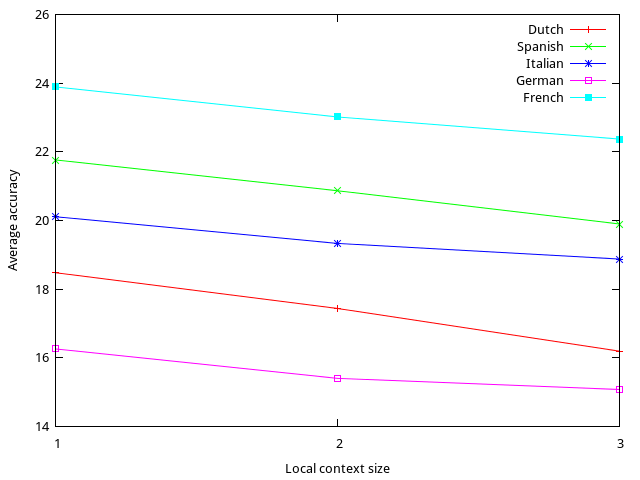
\includegraphics[width=8cm]{context.png}
}
\caption{Average accuracy for different local context sizes}
\label{figcontext}
\end{figure}

We submitted three configurations of our system to the shared task, the maximum
number of runs. Adding lemma features to the local context window of three
words, i.e. left word, focus word and right word, proves beneficial in general.
This is shown in Table~\ref{tab:trialresults}.  This is therefore the first
configuration we submitted (\texttt{c1l}). As second configuration
(\texttt{c1lN}) we submitted the same configuration without parameter
optimisation on the classifiers. Note that neither of these include global
context features.

\begin{table}[t]
\footnotesize
\noindent\makebox[\textwidth][c]{%
\begin{tabular}{lrrrrr}
\hline
\textbf{BEST} & \textbf{ES} & \textbf{FR} & \textbf{IT} & \textbf{NL} & \textbf{DE} \\
\hline
baseline &  19.65 & 21.23 & 15.17 & 15.75 & 13.16 \\
plain & 21.76 & 23.89 & 20.10 & 18.47 & 16.25 \\
$+$lem (\texttt{c1l}) & 21.88 & \textbf{23.93} & \textbf{19.90} & \textbf{18.61} & \textbf{16.43} \\
$+$pos & 22.09 & 23.91 & 19.95 & 18.02 & 15.37 \\
lem$+$pos & \textbf{22.12} & 23.61 & 19.82 & 18.18 & 15.48 \\
glob.context & 20.57 & 23.34 & 17.76 & 17.06 & 16.05 \\
\hline
\textbf{OUT-OF-5} & \textbf{ES} & \textbf{FR} & \textbf{IT} & \textbf{NL} & \textbf{DE} \\
\hline
baseline & 48.34 & 45.99 & 34.51 & 38.59 & 32.90 \\
plain & 49.81 & \textbf{50.91} & 42.30 & 41.74 & \textbf{36.86} \\
$+$lem (\texttt{c1l}) & \textbf{49.91} & 50.65 & \textbf{42.41} & \textbf{41.83} & 36.45 \\
$+$pos & 47.86 & 49.72 & 41.91 & 41.31 & 35.93 \\
lem$+$pos & 47.90 & 49.75 & 41.49 & 41.31 & 35.80 \\
glob.context & 48.09 & 49.68 & 40.87 & 37.70 & 34.47 \\
\hline
\end{tabular}}
\caption{Feature exploration on the trial data}
\label{tab:trialresults}
\end{table}

The third configuration (\texttt{var}) we submitted includes feature selection,
and selects per word expert the configuration that has the highest score on the
trial data, and thus tests all kinds of configurations. Note that
hyperparameter optimisation is also enabled for this configuration. Due to the
feature selection on the trial data, we by definition obtain the highest scores
on this trial data, but this carries the risk of overfitting. Results on the
trial data are shown in Table~\ref{tabpar}.

\begin{table}
\footnotesize
\noindent\makebox[\textwidth][c]{%
\begin{tabular}{lrrrrr}
\hline
\textbf{BEST} & \textbf{ES} & \textbf{FR} & \textbf{IT} & \textbf{NL} & \textbf{DE} \\
\hline
c1lN & 22.60  & 24.09 & 19.87 & 18.70 & 16.43 \\
c1l & 21.88 & 23.93 & 19.90 & 18.61 & 16.43 \\
var & 23.79 & \textbf{25.66} & \textbf{21.65} & \textbf{20.19} & \textbf{19.06} \\
varN & \textbf{23.90} &  25.65 & 21.52 & 19.92 & 18.96 \\
\hline
\textbf{OUT-OF-5} &  \textbf{ES} & \textbf{FR} & \textbf{IT} & \textbf{NL} & \textbf{DE} \\
\hline
c1lN & 50.14 & 50.98 & 42.92 & 42.08 &  36.45 \\
c1l & 49.91 & 50.65 & 42.41 & 41.83 & 36.45 \\
var & 51.95 & \textbf{53.66} & 45.59 & \textbf{44.66} & \textbf{39.81} \\
varN & \textbf{52.91} & 53.61 & \textbf{45.92} & 44.32 & 39.40 \\
\hline
\end{tabular}}
\caption{Results on the trial data}
\label{tabpar}
\end{table}

The hyperparameter optimisation on classifier accuracy has a slightly negative
impact, suggesting overfitting on the training data. Therefore a fourth
configuration (\texttt{varN}) was tried later to independently assess the idea
of feature selection, without hyperparameter optimisation on the classifiers.
This proves to be a good idea. However, the fourth configuration was not yet
available for the actual competition. This incidentally would have had no
impact on the final ranking between competitors. When we run these systems on
the actual test data of the shared task, we obtain the results in
Table~\ref{tabfinal}. The best score amongst the other competitors is mentioned
in the last row for reference, this is the HLTDI team \citep{HLTDI} for all but
Best-Spanish, which goes to the NRC contribution \citep{CARPUAT}.

\begin{table}[tbh]
\footnotesize
\noindent\makebox[\textwidth][c]{%
\begin{tabular}{lrrrrr}
\hline
\textbf{BEST} & \textbf{ES} & \textbf{FR} & \textbf{IT} & \textbf{NL} & \textbf{DE} \\
\hline
baseline & 23.23 & 25.74 & 20.21 & 20.66 & 17.42 \\
c1l &  28.40 & 29.88 & 25.43 & 23.14 & 20.70 \\
c1lN &  28.65 & 30.11 & \textbf{25.66} & \textbf{23.61} & 20.82 \\
var & 23.3 & 25.89 & 20.38 & 17.17 & 16.2 \\
varN & 29.05 & \textbf{30.15} & 24.90 & 23.57 & \textbf{21.98} \\
best competitor & \textbf{32.16} & 28.23 & 24.62 & 22.36 & 19.92 \\
\hline
\textbf{OUT-OF-5} & \textbf{ES} & \textbf{FR} & \textbf{IT} & \textbf{NL} & \textbf{DE} \\
\hline
baseline & 53.07 & 51.36 & 42.63 & 43.59 & 38.86 \\
c1l &  58.23 & 59.07 & 52.22 & \textbf{47.83} & 43.17 \\
c1lN & 57.62 & \textbf{59.80} & 52.73 & 47.62 & 43.24 \\
var & 55.70 & 59.19 & 51.18 & 46.85 & 41.46 \\
varN & 58.61 & 59.26 & 50.89 & 50.42 & 43.34 \\
best competitor & \textbf{61.69} & 58.20 & \textbf{53.57}  & 46.55 & \textbf{43.66} \\
\hline
\end{tabular}}
\caption{Results on the test set}
\label{tabfinal}
\end{table}

A major factor in this task is the accuracy of lemmatisation, and to lesser
extent of PoS tagging. We conducted additional experiments on German and French
without lemmatisation, tested on the trial data. Results immediately fell below
baseline.

Another main factor is the quality of the word alignments, and the degree to
which the found word alignments correspond with the translations the human
annotators could choose from in preparing the gold standard. An idea we tested
is, instead of relying on the mere intersection of word alignments, to use a
phrase-translation table generated by and for the Statistical Machine
Translation system Moses \citep{Koehn+07}, which uses the grow-diag-final
heuristic to extract phrase pairs. This results in more phrases, and whilst
this is a good idea for MT, in the current task it has a detrimental effect, as
it creates too many translation options and we do not have an MT decoder to
discard ineffective options in this task. The grow-diag-final heuristic
incorporates unaligned words to the end of a translation in the translation
option, a bad idea for CLWSD.


\section{Discussion and Conclusion}

%Cross-Lingual Word Sense Disambiguation and Cross-Lingual Lexical Substitution
%have proven to be hard tasks, with scores that are relatively close to
%baseline.


%It has to be noted that the approach laid out here is built around word
%experts. Some word experts may perform well in a certain configuration, and
%others may perform worse. This is also a more general fact: some words seem
%notably harder than others, and perform worse in any configuration.

In our UvT-WSD1 system, we used the same configuration of feature extraction,
or a voter over a predetermined set of configurations, for all word experts. The actual
classifier parameters however, do differ per word expert, as they are the
result of the automatic parameter optimisation algorithm. Our WSD2 system
takes parameter optimisation one step further by selecting system parameters
per word expert from the best configurations on the trial data. Optimising the
hyperparameters of the classifiers on the training data proves to have a
slightly negative effect though, especially when combined with the selection of
features. This is likely due to the fact that feature selection was performed
after hyperparameter optimisation, causing certain optimisations to be rendered
ineffective.

Keeping in mind the fact that different word experts may perform differently,
some \emph{general} conclusions can be drawn from the experiments on the trial
data. It appears to be beneficial to include lemma features, rather than just
word features. Both the 2010 and 2013 tasks corroborate this. However, adding
Part-of-Speech features tends to have a negative impact. For these local
context features, the optimum context size is often two features to the left
and two features to the right of the focus word, cf.  \cite{Hendrickx+02}.

The global keyword features perform well for UvT-WSD1, but best results are
achieved if they are not mixed with the local context features in one
classifier. For WSD2 in the 2013 task, however, the global context features
make less an impact than even just the linguistically-uninformed local context
feature, as became clear from the the feature exploration stage in
Table~\ref{tab:trialresults}. As the keyword selection algorithm is the same
as in UvT-WSD1, this is surprising and must then be attributed to the dataset.
Taking into account the earlier discrepancy between the results of UvT-WSD1 and
WSD2, we may conclude that optimal configurations differ accross datasets.

For UvT-WSD1, an arbiter voting approach over multiple classifiers helps to smooth out errors
and yields the highest scores (see Tables \ref{tab:uvtwsd1clls} and
\ref{tab:uvtwsd1clwsd}). When compared to the other
participants, the UvT-WSD1 system in the voting configuration ranks first in
the Word Sense Disambiguation task, for the two language pairs in which we
participated. WSD2 does not use a voting approach, as it already explicitly
attempts to assess the efficacy of various hyperparameter optimisations and
feature selections.

When asked to predict the best translation(s), our WSD2 system comes out on top
for four out of five languages in the SemEval 2013 task; only for Spanish we
are surpassed by two competitors. Our out-of-five predictions win for two out
of five languages, and are fairly close the the best competitor for the others,
except again for Spanish. It is interesting to observe that, due to our feature
selection without hyperparameter optimisation on the classifier not being
available yet at the time of submission, our simplest system \texttt{c1lN}
emerged as best in the contest.

We assumed independence between hyperparameter optimisation and feature
selection, where the former was conducted using cross-validation on the
training data rather than on the development set. As this independence
assumption is a mere simplification to reduce algorithmic complexity, future
research could focus on a more integrated approach and test hyperparameter
optimisation of the classifiers on the trial set which may produce better
scores.

The WSD2 system is available as open-source under the GNU Public License v3. It
is implemented in Python \citep{PYTHON} and can be obtained from
\url{https://github.com/proycon/wsd2}\footnote{git commit
f10e796141003d8a2fbaf8c463588a6d7380c05e represents a fair state of the system
at the time of submission}. The experimental data and output of our
participation in the 2013 SemEval task are included in
this git repository as well.


\chapter{Translation Assistance by Translation of L1 Fragments in an L2 Context}
\title{Translation of L1 Fragments in an L2 Context}
\label{chap:colibritapilot}

In this chapter we present new research in translation assistance. We
describe a pilot system capable of translating native language (L1)
fragments to foreign language (L2) fragments in an L2
context. Practical applications of this research can be framed in
the context of second language learning.  The type of translation
assistance system under investigation here encourages language
learners to write in their target language while allowing them to
fall back to their native language in case the correct word or
expression is not known. These code switches are subsequently
translated to L2 given the L2 context.  We study the
feasibility of exploiting cross-lingual context to obtain
high-quality translation suggestions that improve over statistical
language modelling and word-sense disambiguation baselines. A
classification-based approach is presented that is indeed found to
improve significantly over these baselines by making use of a
contextual window spanning a small number of neighbouring words.

\nobibliography*
\textsc{This chapter is based on: }
\begin{NoHyper}\bibentry{COLIBRITAPILOT}\end{NoHyper}



\section{Introduction}

Whereas machine translation generally concerns the translation of
whole sentences or texts from one language to the other, this study
focusses on the translation of native language (henceforth L1) words
and phrases, i.e. smaller fragments, in a foreign language (L2)
context. Despite the major efforts and improvements, automatic
translation does not yet rival human-level quality. Vexing issues are
morphology, word-order change and long-distance dependencies. Although
there is a morpho-syntactic component in this research, our
scope is more constrained; its focus is on the faithful preservation
of meaning from L1 to L2, akin to the role of the translation model in
Statistical Machine Translation (SMT).
%Our problem is therefore
%more localised compared to SMT and thus evades some of the additional
%complexities in the syntactic domain.

The cross-lingual context in our research question may at first seem
artificial, but its design explicitly aims at applications related to
computer-aided language learning \citep{CALL2,CALL} and computer-aided
translation \citep{CAT}. Currently, language learners need to refer to a
bilingual dictionary when in doubt about a translation of a word or phrase.
Yet, this problem arises in a context, not in isolation; the learner may have
already translated successfully a part of the text into L2 leading up to the
problematic word or phrase. Dictionaries are not the best source to look up
context; they may contain example usages, but remain biased towards single
words or short expressions.

The proposed application allows code switching and produces context-sensitive
suggestions as writing progresses. In this research we test the feasibility of
the foundation of this idea.The following examples serve to illustrate the idea
and demonstrate what output the proposed translation assistance system would
ideally produce. The parts in bold correspond to respectively the inserted
fragment and the system translation.

\begin{itemize}
  \item
    Input (L1=English,L2=Spanish): \emph{“Hoy vamos a \textbf{the swimming
    pool}.”} \\
    Desired output: \emph{“Hoy vamos a \textbf{la piscina}.”}
  \item
    Input (L1-English, L2=German): \emph{“Das wetter ist wirklich
    \textbf{abominable}.”} \\
    Desired output: \emph{“Das wetter ist wirklich \textbf{ekelhaft}.”}
  \item
    Input (L1=French,L2=English): \emph{“I \textbf{rentre à la maison} because
    I am tired.”} \\
    Desired output: \emph{“I \textbf{return home} because I am tired.”}
  \item
    Input (L1=Dutch, L2=English): \emph{“Workers are facing a massive \textbf{aanval
    op} their employment and social rights.”} \\
    Desired output: \emph{“Workers are facing a massive \textbf{attack on}
    their employment and social rights.”}
\end{itemize}


The main research question in this research is how to disambiguate an L1 word
or phrase to its L2 translation based on an L2 context, and whether such
cross-lingual contextual approaches provide added value compared to baseline
models that are not context informed or compared to standard language models.



\section{Data preparation}

Preparing the data to build training and test data for our intended
translation assistance system is not trivial, as the type of
interactive translation assistant we aim to develop does not exist yet. We
need to generate training and test data that realistically emulates
the task. We start with a parallel corpus that is tokenised for both
L1 and L2. No further linguistic processing such as part-of-speech
tagging or lemmatisation takes place in our experiments; adding this
remains open for future research.
% and may likely lead to further
%improvements in the results.

The parallel corpus is randomly sampled into two large and
equally-sized parts. One is the basis for the training set, and the
other is the basis for the test set. The reason for such a large test
split shall become apparent soon.

From each of the splits ($S$), a phrase-translation table is constructed
automatically in an unsupervised fashion. This is done using the scripts
provided by the Statistical Machine Translation system Moses \citep{MOSES}. It
invokes GIZA++ \citep{GIZA} to establish statistical word alignments based on
the IBM Models and subsequently extracts phrases using the
\texttt{grow-diag-final} algorithm \citep{OchNey2003}. The result, independent
for each set, will be a phrase-translation table ($T$) that maps phrases in L1
to L2. For each phrase-pair ($f_s,f_t$) this phrase-translation table holds the computed
translation probabilities $P(f_s|f_t)$ and $P(f_t|f_s)$.

Given these phrase-translation tables, we can now extract both training data
and test data using the algorithm in Figure~\ref{fig:algo}.  In our discourse, the source language ($s$) corresponds to L1, the
fallback language used for by the end-user for inserting fragments, whilst the
target language ($t$) is L2.

\begin{figure}[t]
\begin{framed}
\begin{enumerate}
%\footnotesize
\item using phrase-translation table $T$ and parallel corpus split $S$
\item \textbf{for} each aligned sentence pair $({sentence}_s \in
  S_s,{sentence}_t \in S_t)$ in the parallel corpus split ($S_s$,$S_t$):
\item \hspace{5mm}\textbf{for} each fragment $(f_s \in {sentence}_s, f_t \in
  {sentence}_t)$ where $(f_s, f_t) \in T$:
\item \hspace{10mm}\textbf{if} $P(f_s|f_t) \cdot P(f_t|f_s) \geq \lambda_1$
  \textbf{and} $P(f_s|f_t) \cdot P(f_t|f_s) \geq
  \lambda_2 \cdot P(f_s|f_{strongest\_t}) \cdot  P(f_{strongest\_t}|f_s)$:
\item \hspace{15mm}Output a pair $({sentence}_t',{sentence}_t)$ where
  ${sentence}_t'$ is a copy of $t$ but with
  fragment $f_t$ substituted by $f_s$, i.e. the introduction of an L1 word or phrase in an L2 sentence.
\end{enumerate}
\end{framed}
\caption{Algorithm for extracting training and test data on the basis of a
phrase-translation table ($T$) and subset/split from a parallel corpus ($S$).
The indentation indicates the nesting.}
\label{fig:algo}
\end{figure}

Step 4 is effectively a filter: two thresholds can be configured to discard
weak alignments, i.e. those with low probabilities, from the phrase-translation
table so that only strong couplings make it into the generated set. The
parameter $\lambda_1$ adds a constraint based on the product of the two
conditional probabilities $(P(f_t|f_s) \cdot P(f_s|f_t))$, and sets a threshold
that has to be surpassed.  A second parameter $\lambda_2$  further limits the
considered phrase pairs $(f_s,f_t)$ to have the product of their conditional
probabilities not deviate more than a fraction $\lambda_2$ from the joint
probability for the strongest possible pairing for $f_s$, the source fragment.
In Figure~{fig:algo}, $f_{strongest\_t}$ corresponds to the best scoring
translation for a given source fragment $f_s$. This metric thus effectively
prunes weaker alternative translations in the phrase-translation table from
being considered if there is a much stronger candidate. Nevertheless, it has to
be noted that even with $\lambda_1$ and $\lambda_2$, the test set will include
a certain amount of errors. This is due to the nature of the unsupervised
method with which the phrase-translation table is constructed. For our purposes
however, the test set suffices to test our hypothesis.

In our experiments, we choose fixed values for these parameters, by
manual inspection and judgement of the output. The $\lambda_1$
parameter was set to $0.01$ and $\lambda_2$ to $0.8$.  Whilst other
thresholds may possibly produce cleaner sets, this is hard to evaluate
as finding optimal values causes a prohibitive increase in complexity
of the search space, and again this is not necessary to test our hypothesis.

The output of the algorithm in Figure~\ref{fig:algo} is a modified set of sentence pairs
$({sentence}_t',{sentence}_t)$, in which the same sentence pair may be used multiple times
with different L1 substitutions for different fragments.
%A single L2
%sentence $t$ may thus occur in multiple sentence pairs.
The final
test set is created by randomly sampling the desired number of test
instances.

Note that the training set and test set are constructed on their own
respective and independently generated phrase-translation tables. This
ensures complete independence of training and test data. Generating
test data using the same phrase-translation table as the training data
would introduce a bias. The fact that a phrase-translation table needs
to be constructed for the test data is also the reason that the
parallel corpus split from which the test data is derived has to be
large enough, ensuring better quality.

We concede that our current way of testing is a mere approximation of the real-world scenario. An ideal test corpus
would consist of L2 sentences with L1 fallback as crafted by L2 language learners with an L1 background. However, such
corpora do not exist yet at the time of this research. Nevertheless, we hope to show that our automated way of test set
generation is sufficient to test the feasibility of our core hypothesis that L1 fragments can be translated to L2 using
L2 context information.

\section{System}

We develop a classifier-based system composed of so-called ``classifier
experts''. Numerous classifiers are trained and each is an expert in
translating a single word or phrase. In other words, for each word type or
phrase type that occurs as a fragment in the training set, and which does not
map to just a single translation, a classifier is trained.  The classifier maps
the L1 word or phrase in its L2 context to its L2 translation. Words or phrases
that always map to a single translation are stored in a simple mapping table,
as a classifier would have no added value in such cases. The classifiers use
the IB1 algorithm \citep{IB1} as implemented in TiMBL
\citep{TIMBL}.\footnote{\url{https://languagemachines.github.io/timbl}} IB1 implements
$k$-nearest neighbour classification. The choice for this algorithm is
motivated by the fact that it handles multiple classes with ease, but first and
foremost because it has been successfully employed for word sense
disambiguation in other studies \citep{Hoste+02,GAMBL}, in particular in
cross-lingual word sense disambiguation as seen in Chapter~\ref{chap:clwsd}. It has
also been used in machine translation studies in which local source context is
used to classify source phrases into target phrases, rather than looking them
up in a phrase table \citep{Stroppa+07,Haque+11}. The idea of local phrase
selection with a discriminative machine learning classifier using additional
local (source-language) context was introduced in parallel to \cite{Stroppa+07} by \cite{Carpuat+07} and
\cite{Gimenez+07}; cf. \cite{Haque+11} for an overview of more recent methods.

The feature vector for the classifiers represents a local context of
neighbouring words, and optionally also global context keywords in a
binary-valued bag-of-words configuration. The local context consists
of an $X$ number of L2 words to the left of the L1 fragment, and $Y$
words to the right.

When presented with test data, in which the L1 fragment is explicitly marked,
we first check whether there is ambiguity for this L1 fragment and if a direct
translation is available in our simple mapping table. If so, we are done
quickly and need not rely on context information. If not, we check for the
presence of a classifier expert for the offered L1 fragment; only then we can
proceed by extracting the desired number of L2 local context words to the
immediate left and right of this fragment and adding those to the feature
vector. The classifier will return a probability distribution of the most likely
translations given the context and we can replace the L1 fragment with the
highest scoring L2 translation and present it back to the user.

In addition to local context features, we also experimented with
global context features. These are a set of L2 contextual keywords for
each L1 word/phrase and its L2 translation occurring in the same
sentence, not necessarily in the immediate neighbourhood of the L1
word/phrase. The keywords are selected to be indicative for a specific
translation. We used the method of extraction by \cite{NgL96}, as we have seen in Chapter~\ref{chap:clwsd}, and
encoded all keywords in a binary bag of words model. The experiments
however showed that inclusion of such keywords did not make any
noticeable impact on any of the results, so we restrict ourselves to
mentioning this negative result.

%<paraphrase from earlier paper>
%In addition to this, {\em global context}\/ features may be extracted; these are
%a set of L2 keywords per L1 word/phrase and its L2 translation. The keywords
%have to be found occurring above certain occurrence thresholds at arbitrary
%positions in the same sentence. The global context features are represented as
%a binary bag-of-words model in which the presence of each of the keywords that
%may be indicative for a given mapping of the focus word/phrase to a translation
%is represented by a boolean value. Such a set of keywords is constructed
%independently for each classifier. For some classifiers no keywords
%may be found.

%The method used to extract these keywords ($k$) is proposed by
%\newcitep{NgL96}.
%Assume we have a fragment $f$, more precisely, an
%L1 word or phrase.  We also have one of its aligned L2 translations
%$s$. We can now estimate $P(s|k)$, the probability of translation $s$,
%given an L2 keyword $k$. Let $N_{s,k_{local}.}$ be the number of
%occurrences of a possible context word $k$ pertaining to a particular
%combination of L1 fragment and L2 translation $s$. Let $N_{k_{local}}$
%be the number of occurrences of a possible local context keyword $k$
%pertaining to a particular L1 fragment but regardless of its
%translation. If we also take into account the frequency of a possible
%keyword $k$ in the complete training corpus ($N_{k_{corpus}}$), we
%get:

%\begin{equation}
%P(s|k) = \frac{N_{s,k_{local}}}{N_{k_{local}}}(\frac{1}{N_{k_{corpus}}})
%\end{equation}

%\newcitep{Hoste+02} select a keyword $k$ for inclusion in the bag-of-words
%representation if that keyword occurs more than $T_1$ times in that translation
%$s$, and if $P(s|k) \ge T_2$. Both $T_1$ and $T_2$ are predefined thresholds,
%which by default were set to $3$ and $0.001$ respectively. We adopted these same
%values.

%The selection of bag-of-word features is computed prior to the
%extraction of the training instances, as this information is a prerequisite for
%the successful generation of both training and test instances.
%</paraphrase from earlier paper>

Our full system, including the scripts for data preparation, training, and
evaluation, is implemented in Python and freely available as open-source from
\url{https://github.com/proycon/colibrita/} . Version tag \texttt{v0.2.1} is
representative for the version used in this research.


\subsection{Language Model}

%This led us to
We also implement a statistical language model as an optional component of our
classifier-based system and also as a baseline to compare our system to.  The
language model is a trigram-based back-off language model with Kneser-Ney
smoothing, computed using SRILM \citep{SRILM} and trained on the same training
data as the translation model. No additional external data was brought in, to
keep the comparison fair.

For any given hypothesis $H$, results from the L1 to L2 classifier are combined with
results from the L2 language model. We do so by normalising the class
probability from the classifier ($score_T(H)$), which is our translation model, and the language model
($score_{lm}(H)$), in such a way that the highest classifier score for
the alternatives under consideration is always $1.0$, and the highest
language model score of the sentence is always $1.0$. Take $score_T(H)$
and $score_{lm}(H)$ to be log probabilities, the search for the best (most
probable) translation hypothesis $\hat{H}$ can then be expressed as:

\begin{equation}
  \hat{H} = \arg\max_H (score_T(H) + score_{lm}(H))
  \label{eq:LM}
\end{equation}

If desired, the search can be parametrised with variables $\lambda_3$ and
$\lambda_4$, representing the weights we want to attach to the classifier-based
translation model and the language model, respectively. In the current study we
simply left both weights set to one, thereby assigning equal importance to
translation model and language model.

%\begin{equation}
%  \arg\max_B = \lambda_3 score_T + \lambda_4 score_{lm}
%\end{equation}

% maar deze equation is dan eigenlijk een beetje overbodig...
%da's waar,  weggehaald, scheelt weer ruimte

\section{Evaluation}

Several automated metrics exist for the evaluation of L2 system
output against the L2 reference output in the test set. We first
measure absolute accuracy by simply counting all output fragments that
exactly match the reference fragments, as a fraction of the total
amount of fragments. This measure may be too strict, so we add a more
flexible \emph{word accuracy} measure which takes into account partial
matches at the word level. If output $o$ is a subset of reference $r$
then a score of $\frac{|o|}{|r|}$ is assigned for that sentence
pair. If instead, $r$ is a subset of $o$, then a score of
$\frac{|r|}{|o|}$ will be assigned. A perfect match will result
in a score of $1$ whereas a complete lack of overlap will be
scored $0$. The word accuracy for the entire set is then computed by
taking the sum of the word accuracies per sentence pair, divided by
the total number of sentence pairs.

We also compute a recall metric that measures the number of fragments that the
system provided a translation for as a fraction of the total number of
fragments in the input, regardless of whether the fragment is translated
correctly or not. The system may skip fragments for which it can find no
solution at all.

In addition to these, the system's output can be compared against the
L2 reference translation(s) using established Machine Translation
evaluation metrics.  We report on BLEU, NIST, METEOR, and word error
rate metrics WER and PER.  These scores should generally be much
better than the typical MT system performances as only local changes
are made to otherwise ``perfect'' L2 sentences.

\section{Baselines}

A context-insensitive yet informed baseline was constructed to assess
the impact of L2 context information in translating L1 fragments. The
baseline selects the most probable L1 fragment per L2 fragment
according to the phrase-translation table. This baseline, henceforth
referred to as the 'most likely fragment' baseline (MLF) is analogous
to the 'most frequent sense'-baseline common in evaluating WSD
systems.

A second baseline was constructed by weighing the probabilities from
the translation table directly with the L2 language model described
earlier. It adds a LM component to the MLF baseline. This LM baseline
allows the comparison of classification through L1 fragments in an L2
context, with a more traditional L2 context modelling (i.e. target
language modelling) which is also customary in MT decoders. Computing
this baseline is done in the same fashion as previously illustrated in
Equation~\ref{eq:LM}, where $score_T$ then represents the normalised
$p(t|s)$ score from the phrase-translation table rather than the class
probability from the classifier.

\section{Experiments \& Results}

The data for our experiments were drawn from the Europarl parallel corpus
\citep{EUROPARL} from which we extracted two sets of $200,000$ sentence
pairs each for several language pairs. These were used to form the
training and test sets. The final test sets are a randomly sampled
$5,000$ sentence pairs from the $200,000$-sentence test split for each
language pair.

All input data for the experiments in this section are publicly available\footnote{Download and
unpack \url{http://lst.science.ru.nl/~proycon/colibrita-acl2014-data.zip}}.

Let us first zoom in to convey a sense of scale on a specific
language pair. The actual Europarl training set we generate for
English (L1) to Spanish (L2), i.e. English fallback in a Spanish
context, consists of $5,608,015$ sentence pairs. This number is much
larger than the $200,000$ we mentioned before because single sentence
pairs may be reused multiple times with different marked fragments.
From this training set of sentence pairs over $100,000$ classifier
experts are derived. The eleven largest classifiers are shown in
Table~\ref{tab:topexperts}, along with the number of training
instances per classifier. The full table would reveal a Zipfian
distribution.

\begin{table}[hbt]
\footnotesize
\noindent\makebox[\textwidth][c]{%
\begin{tabular}{lll}
\hline
Fragment & Training instances & Translations \\
\hline
the & 256,772 & la, el, los, las  \\
of &   139,273 & de, del \\
and &  128,074 & y, de, e \\
to &   66,565 & a, para, que, de \\
a &  54,306 & un, una \\
is &  40,511 & es, está, se \\
for & 34,054 & para, de, por \\
this & 29,691 & este, esta, esto \\
European & 26,543 & \pbox{3cm}{Europea, Europeo \\ Europeas, Europeos} \\
on & 23,147 & sobre, en \\
of the & 22,361 & de la, de los\\
\hline
\end{tabular}}
\caption{The top eleven classifier experts for English to Spanish. The eleventh
entry is included as an example of a common phrasal fragment}
\label{tab:topexperts}
\end{table}

Among the classifier experts are only words and phrases that are
ambiguous and may thus map to multiple translations. This implies that
such words and phrases must have occurred at least twice in the
corpus, though this threshold is made configurable and could have been
set higher to limit the number of classifiers. The remaining $246,380$
unambiguous mappings are stored in a separate mapping table.

For the classifier-based system, we tested various different feature
vector configurations. The first experiment, of which the results are
shown in Figure~\ref{fig:context}, sets a fixed and symmetric local
context size across all classifiers, and tests three context
widths. Here we observe that a context width of one yields the best
results. The BLEU scores, not included in the figure but shown in
Table~\ref{tab:results}, show a similar trend. This trend holds for
all the MT metrics.

%It is also worth noting that as
%expected, all metrics correlate as they all measure essentially the
%same thing; overlap between the system output and the reference
%translation in the test set, but in different ways and focussing on
%different aspects.

Table~\ref{tab:results} shows the results for English to Spanish in
more detail and adds a comparison with the two baseline systems. The various
\texttt{lXrY} configurations use the same feature vector setup for all classifier
experts. Here $X$ indicates the left context size and $Y$ the right context
size.
%Each of these configurations uses the same feature
%vector setup across all classifier experts
The \texttt{auto} configuration
does not uniformly apply the same feature vector setup to all classifier
experts but instead seeks to find the optimal setup per
classifier expert. This shall be further discussed in
Section~\ref{sec:optim}.

\begin{figure}[t]
\centering
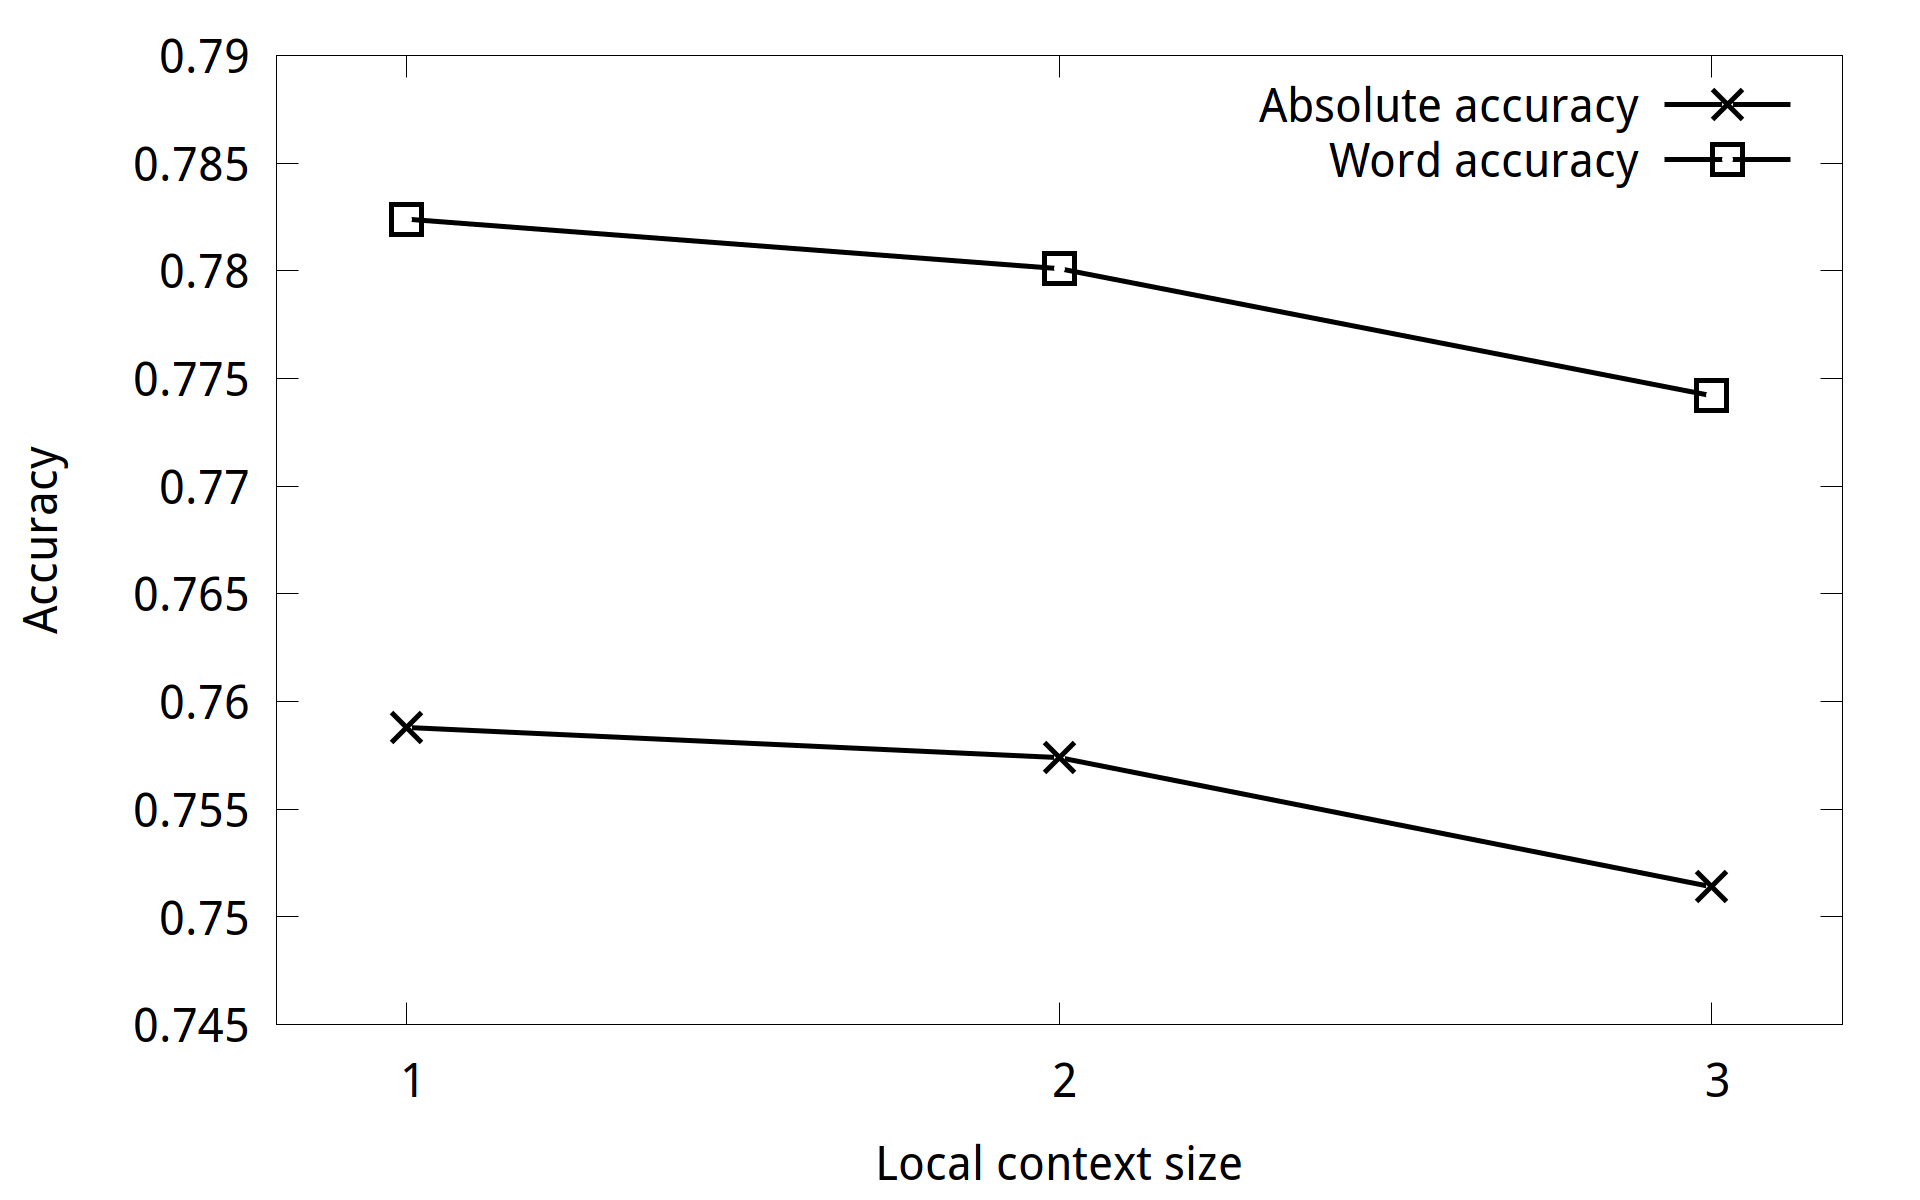
\includegraphics[width=10cm]{colibritapilot-context.png}
\caption{Accuracy for different local context sizes, Europarl English to Spanish}
\label{fig:context}
\end{figure}



\begin{center}
\begin{table*}[bt]
%\footnotesize
\noindent\makebox[\textwidth][c]{%
\begin{tabular}{llllllll}
\hline
Configuration & Accuracy & Word Accuracy & BLEU & METEOR & NIST & WER & PER \\
\hline
MLF baseline & 0.6164 & 0.6662 & 0.972 & 0.9705 & 17.0784 & 1.4465 & 1.4209 \\
LM baseline & 0.7158 & 0.7434 & 0.9785 & 0.9739 & 17.1573 & 1.1735 & 1.1574 \\
\hline
l1r1 & 0.7588 & 0.7824  & 0.9801 & 0.9747 & 17.1550 & 1.1625 & 1.1444 \\
l2r2 & 0.7574 & 0.7801 & 0.9800 & 0.9746 & 17.1550 & 1.1750 & 1.1569 \\
l3r3 & 0.7514 & 0.7742 & 0.9796 & 0.9744 & 17.1445 & 1.1946 & 1.1780 \\
\hline
l1r1$+$LM & \textbf{0.7810} & \textbf{0.7973} & \textbf{0.9816} &
\textbf{0.9754} & \textbf{17.1685} & \textbf{1.0946} & \textbf{1.077} \\
\hline
%l1r1k & 0.7586 & 0.7823 & 0.9801 & 0.9747 & 17.1548 & 1.1630 & 1.1449 \\
%\hline
auto & 0.7626 & 0.7850 & 0.9803 & 0.9748 & 17.1544 & 1.1594 & 1.1424 \\
auto$+$LM & 0.7796 & 0.7966 & 0.9815 & 0.9754 & 17.1664 & 1.1021 & 1.0845 \\
\hline
l1r0 & 0.6924 & 0.7223 & 0.9757 & 0.9723 & 17.1087 & 1.3415 & 1.3249\\
l2r0 & 0.6960 & 0.7245 & 0.9759 & 0.9724 & 17.1091 & 1.3364 & 1.3193\\
l2r1 & 0.7624 & 0.7849 & 0.9803 & 0.9748 & 17.1558 & 1.1554 & 1.1378\\
\hline
\end{tabular}}
\caption{Europarl results for English to Spanish (i.e English fallback in
Spanish context). Recall $ = 0.9422$}
\label{tab:results}
\end{table*}
\end{center}


As expected, the LM baseline substantially outperforms the
context-insensitive MLF baseline. Second, our classifier approach
attains a substantially higher accuracy than the LM baseline. Third,
we observe that adding the language model to our classifier leads to
another significant gain (configuration \texttt{l1r1$+$LM} in the
results in Table~\ref{tab:results}).  It appears that the classifier
approach and the L2 language model are able to complement each other.

Statistical significance on the BLEU scores was tested using pairwise bootstrap
sampling \citep{KoehnStatSig}.  All significance tests were performed with
$5,000$ iterations.  We compared the outcomes of several key configurations. We
first tested \texttt{l1r1} against both baselines; both differences are
significant at $p<0.01$ for both. The same significance level was found when
comparing \texttt{l1r1$+$LM} against \texttt{l1r1}, \texttt{auto$+$LM} against
\texttt{auto}, as well as the LM baseline against the MLF baseline. Automatic
feature selection \texttt{auto} was found to perform statistically better than
\texttt{l1r1}, but only at $p<0.05$. Conclusions with regard to context width
may have to be tempered somewhat, as the performance of the \texttt{l1r1}
configuration was found to not be significantly better than that of the
\texttt{l2r2} configuration. However, \texttt{l1r1} performs significantly
better than \texttt{l3r3} at $p<0.01$, and \texttt{l2r2} performs significantly
better than \texttt{l3r3} at $p<0.01$.

% ~/mtevalscripts/paired_bootstrap_v13a/paired_bootstrap_resampling_bleu_v13a.pl pb_l1r1.statsfile pb_baseline.statsfile 5000 0.05
%System 1 BLEU better: 5000 / 5000 = 1 -- BLEU SIGNIFICANT at p = 0.05                                                                               │···················

%~/mtevalscripts/paired_bootstrap_v13a/paired_bootstrap_resampling_bleu_v13a.pl pb_l1r1lm.statsfile pb_l1r1.statsfile 5000 0.05
% System 1 BLEU better: 5000 / 5000 = 1 -- BLEU SIGNIFICANT at p = 0.05

%~/mtevalscripts/paired_bootstrap_v13a/paired_bootstrap_resampling_bleu_v13a.pl pb_lmbaseline.statsfile pb_baseline.statsfile 5000 0.05
% System 1 BLEU better: 5000 / 5000 = 1 -- BLEU SIGNIFICANT at p = 0.05

% ~/mtevalscripts/paired_bootstrap_v13a/paired_bootstrap_resampling_bleu_v13a.pl pb_al5r5k.statsfile pb_l1r1.statsfile 5000 0.05
%System 1 BLEU better: 4818 / 5000 = 0.9636 -- BLEU SIGNIFICANT at p = 0.05

%~/mtevalscripts/paired_bootstrap_v13a/paired_bootstrap_resampling_bleu_v13a.pl pb_al5r5klm.statsfile pb_al5r5k.statsfile 5000 0.05
%System 1 BLEU better: 5000 / 5000 = 1 -- BLEU SIGNIFICANT at p = 0.05

%proycon@scootaloo /scratch/proycon/colibrita/2/europarl200k-en-es$ ~/mtevalscripts/paired_bootstrap_v13a/paired_bootstrap_resampling_bleu_v13a.pl pb_l1r1lm.statsfile pb_al5r5k.statsfile 5000 0.05
%System 1 BLEU better: 5000 / 5000 = 1 -- BLEU SIGNIFICANT at p = 0.05

%~/mtevalscripts/paired_bootstrap_v13a/paired_bootstrap_resampling_bleu_v13a.pl pb_l1r1.statsfile pb_l2r2.statsfile 5000 0.05    master 16:05:04
%System 1 BLEU better: 4159 / 5000 = 0.8318

%l1 over l3
%System 1 BLEU better: 4994 / 5000 = 0.9988 -- BLEU SIGNIFICANT at p = 0.05

%l2 over l3
%System 1 BLEU better: 4998 / 5000 = 0.9996 -- BLEU SIGNIFICANT at p = 0.05



In Table~\ref{tab:example} we present some illustrative examples from
the English $\rightarrow$ Spanish Europarl data. We show the difference
between the most-likely-fragment baseline and our system.

\begin{table*}[htb]
\begin{framed}
\footnotesize
\textbf{Input:} Mientras no haya prueba en contrario , la financiación de partidos políticos \textbf{European} sólo se justifica , incluso después del tratado de Niza , desde el momento en que concurra a la expresión del sufragio universal , que es la única definición aceptable de un partido político . \\
\textbf{MLF baseline:} Mientras no haya prueba en contrario , la financiación de partidos políticos \textbf{Europea} sólo se justifica , incluso después del tratado de Niza , desde el momento en que concurra a la expresión del sufragio universal , que es la única definición aceptable de un partido político . \\
\textbf{l1r1:} Mientras no haya prueba en contrario , la financiación de partidos políticos \textbf{europeos} sólo se justifica , incluso después del tratado de Niza , desde el momento en que concurra a la expresión del sufragio universal , que es la única definición aceptable de un partido político .\\
\line(1,0){250} \\
\textbf{Input:} Esta Directiva es nuestra oportunidad \textbf{to} marcar una verdadera
diferencia , reduciendo la trágica pérdida de vidas en nuestras carreteras . \\
\textbf{MLF baseline:} Esta Directiva es nuestra oportunidad \textbf{a} marcar una
verdadera diferencia , reduciendo la trágica pérdida de vidas en nuestras
carreteras . \\
\textbf{l1r1:} Esta Directiva es nuestra oportunidad \textbf{para} marcar una
verdadera diferencia , reduciendo la trágica pérdida de vidas en nuestras
carreteras . \\
\line(1,0){250} \\
\textbf{Input:} Es la \textbf{last} vez que me dirijo a esta Cámara . \\
\textbf{MLF baseline:} Es la \textbf{pasado} vez que me dirijo a esta Cámara .\\
\textbf{l1r1:} Es la \textbf{última} vez que me dirijo a esta Cámara .\\
\line(1,0){250} \\
\textbf{Input:} Pero el enfoque actual de la Comisión no puede conducir a una buena
política ya que es tributario del funcionamiento del mercado y de las normas
establecidas por la OMC , el FMI y el Banco Mundial , normas que siguen siendo
desfavorables para los \textbf{developing countries} . \\
\textbf{MLF baseline:} Pero el enfoque actual de la Comisión no puede conducir a
una buena política ya que es tributario del funcionamiento del mercado y de las
normas establecidas por la OMC , el FMI y el Banco Mundial , normas que siguen
siendo desfavorables para los \textbf{los países en desarrollo} . \\
\textbf{l1r1:} Pero el enfoque actual de la Comisión no puede conducir a
una buena política ya que es tributario del funcionamiento del mercado y de las
normas establecidas por la OMC , el FMI y el Banco Mundial , normas que siguen
siendo desfavorables para los \textbf{países en desarrollo} .
\end{framed}
\caption{Some illustrative examples of MLF-baseline output versus system output, in
which system output matches the correct human reference output. The actual fragments
concerned are highlighted in bold. The first example shows our system
correcting for number agreement, the second a correction in selecting the right preposition, and the
third shows that the English word \emph{last} can be translated in different ways, only one of which
is correct in this context. The last example shows a phrasal translation, in
which the determiner was duplicated in the baseline}
\label{tab:example}
\end{table*}

\begin{table*}[htb]
\begin{framed}
\footnotesize
\textbf{Input:} Sin ese tipo de protección la gente no aprovechará la oportunidad \textbf{to} vivir , viajar y trabajar donde les parezca en la Unión Europea . \\
\textbf{l1r1:} Sin ese tipo de protección la gente no aprovechará la oportunidad \textbf{para} vivir , viajar y trabajar donde les parezca en la Unión Europea . \\
\textbf{l1r1$+$LM:} Sin ese tipo de protección la gente no aprovechará la oportunidad \textbf{de} vivir , viajar y trabajar donde les parezca en la Unión Europea . \\
\line(1,0){250} \\
\textbf{Input:} La Comisión también está acometiendo medidas en el ámbito social y \textbf{educational} con vistas a mejorar la situación de los niños . \\
\textbf{l1r1:} La Comisión también está acometiendo medidas en el ámbito social y \textbf{educativas} con vistas a mejorar la situación de los niños .  \\
\textbf{l1r1$+$LM:} La Comisión también está acometiendo medidas en el ámbito social y \textbf{educativo} con vistas a mejorar la situación de los niños . \\
\end{framed}
\caption{Some examples of l1r1 versus the same configuration enriched
  with a language model.}
%The language model version corresponds with the human reference.}
\label{tab:example2}
\end{table*}


Likewise, Table~\ref{tab:example2} exemplifies small fragments from the
\texttt{l1r1} configuration compared to the same configuration enriched with a
language model. We observe in this data that the language model often has the
added power to choose a correct translation that is not the first prediction of
the classifier, but one of the weaker alternatives that nevertheless fits
better.  Though the classifier generally works best in the \texttt{l1r1}
configuration, i.e. with context size one, the trigram-based language model
allows further left-context information to be incorporated that influences the
weights of the classifier output, successfully forcing the system to select
alternatives. This combination of a classifier with context size one and
trigram-based language model proves to be most effective and reaches the best
results so far. We have not conducted experiments with language
models of other orders.

%We initially
%expected the \textbf{auto$+$LM} to obtain better results than
%\textbf{l1r1$+$LM}. However, the complementary effect of classifier
%and language model becomes less pronounced as more context is added to
%the former, taking much of the added value of a language model away.

%We find that the inclusion of global context keywords (the $l1r1k$
%configuration) has no noticeable impact, and this trend holds when
%different language pairs are tested. In one of our English to Dutch
%Europarl sets for example, we find that only $41$ out of $5,000$ test
%sentence pairs trigger a keyword match during testing.  During
%training, keywords were found for $9,910$ out of $112,653$
%classifiers.  The virtually absent impact of global context keywords
%is also in agreement with findings from \newcitep{WSD2}; the trend
%seems to be that simplicity in feature selection pays off and holds
%for all language pairs we tested.

\FloatBarrier

\subsection{Context optimisation}
\label{sec:optim}

It has been argued that classifier experts in a word sense disambiguation
ensemble should be individually optimised \citep{GAMBL}. This we have also shown
in Chapter~\ref{chap:clwsd}, where we find a positive impact when conducting
feature selection per classifier. This intuitively makes sense; a context of
one may seem to be better than any other when uniformly applied to all
classifier experts, but it may well be that certain classifiers benefit from
different feature selections.  We therefore proceed with this line of
investigation as well.

Automatic configuration selection was done by performing leave-one-out
testing (for small number of instances) or 10-fold-cross validation
(for larger number of instances, $n \geq 20$) on the training data per
classifier expert. Various configurations were tested. Per classifier
expert, the best scoring configuration was selected, referred to as
the \texttt{auto} configuration in Table~\ref{tab:results}. The
\texttt{auto} configuration improves results over the uniformly
applied feature selection.  However, if we enable the language model
as we do in the \texttt{auto$+$LM} configuration we do not notice an
improvement over \texttt{l1r1$+$LM}, surprisingly. We suspect the lack
of impact here can be explained by the trigram-based Language Model
having less added value when the (left) context size of the classifier
is two or three; they are now less complementary.

% wat kun je hier meer over zeggen? kun je het verklaren?
% - ik heb een vermoeden, nu hierboven uitgelegd.
%  eventueel zou ik nog experimenten met l2r2LM en l3r3LM kunnen draaien om dit
%  misschien echt hard te kunnen maken.

Table~\ref{tab:autoconf} lists what context sizes have been chosen in the
automatic feature selection. A context size of one prevails in the vast majority of
cases, which is not surprising considering the good results we have already
seen with this configuration.

% hier dan wel iets meer over zeggen, anders mag de lezer raden waarom
% er aandacht en een tabel aan wordt besteed.
% - done, beetje toegevoegd.

\begin{table}[htb]
%\footnotesize
\noindent\makebox[\textwidth][c]{%
\begin{tabular}{rl}
\hline
$66.5\%$ & l1r1\\
$19.9\%$ & l2r2\\
$7.7\%$ & l3r3\\
$3.5\%$ & l4r4\\
$2.4\%$ & l5r5\\
\hline
\end{tabular}}
\caption{Frequency of automatically selected configurations on English to
Spanish Europarl dataset}
\label{tab:autoconf}
\end{table}

In this study we did not yet conduct optimisation of the classifier parameters.
We used the IB1 algorithm with $k=1$ and the default values of the TiMBL
implementation.  In Chapter~\ref{chap:clwsd}, we reported a decrease in
performance due to overfitting when this is done, so we do not expect it to
make a positive impact. The second reason for omitting this is more practical
in nature; to do this in combination with feature selection would add
substantial search complexity, making experiments far more time consuming, even
prohibitively so.

%asymmetry
The bottom lines in Table~\ref{tab:results} represent results when
all right-context is omitted, emulating a real-time prediction when no
right context is available yet. This has a substantial negative impact on
results.
%L1 to L2 translation could first be made using
%such an asymmetric configuration, and the translation choice could be
%revisited and improved when the user continues typing and adds
%right-side context, which improves results substantially.
We experimented with several asymmetric configurations and found that
taking two words to the left and one to the right yields even better results than
symmetric configurations for this data set. This result is in line
with the positive effect of adding the LM to the \texttt{l1r1}.

In order to draw accurate conclusions, experiments on a single data
set and language pair are not sufficient. We therefore conducted a
number of experiments with other language pairs, and present the
abridged results in Table~\ref{tab:results2}.


There are some noticeable discrepancies for some experiments in
Table~\ref{tab:results2} when compared to our earlier results in
Table~\ref{tab:results}. We see that the language model baseline for
English$\rightarrow$French shows the same substantial improvement over the
baseline as our English$\rightarrow$Spanish results.  The same holds for the
Chinese$\rightarrow$English experiment. However, for English$\rightarrow$Dutch
and English$\rightarrow$Chinese we find that the LM baseline actually performs
slightly worse than baseline. Nevertheless, in all these cases, the positive
effect of including a Language Model to our classifier-based system again
shows. Also, we note that in all cases our system performs better than the two
baselines.
%We hypothesise that this may possibly due to the fact that latin languages are
%rich in gender and number agreement, something a language model may solve.
%MAYBE TODO: why is this? (I don't know)

Another discrepancy is found in the BLEU scores of the
English$\rightarrow$Chinese experiments, where we measure an
unexpected drop in BLEU score under baseline. However, all other
scores do show the expected improvement. The error rate metrics show
improvement as well. We therefore attach low importance to this
deviation in BLEU here.

In all of the aforementioned experiments, the system produced a single solution
for each of the fragments, the one it deemed best, or no solution at all if it
could not find any.  Alternative evaluation metrics could allow the system to output
multiple alternatives. Omission of a solution by definition causes a decrease in
recall. In all of our experiments recall is high (well above $90\%$), mostly
because train and test data lie in the same domain and have been generated in
the same fashion, lower recall is expected with more real-world data.

\begin{table}[hbt]
\footnotesize{
\noindent\makebox[\textwidth][c]{%
\begin{tabular}{llllllll}
\hline
Dataset & L1 & L2 & Configuration & Accuracy & Word Accuracy & BLEU \\
\hline
europarl200k & en & nl & baseline & 0.7026 & 0.7283 & 0.9771 \\
europarl200k & en & nl & LM baseline & 0.6958 & 0.7195 & 0.9773\\
europarl200k & en & nl & l1r1 & 0.7790 & 0.7941 & 0.9814 \\
%europarl200k & en & nl & l2r2 & 0.7770 & 0.7926 & 0.9813\\
europarl200k & en & nl & l1r1$+$LM & \textbf{0.7838} & \textbf{0.7973} &
\textbf{0.9818} \\
%europarl200k & en & nl & l1r1k & 0.779 & 0.7941 & 0.9814\\
europarl200k & en & nl & auto & 0.7796 & 0.7947  &0.9815\\
europarl200k & en & nl & auto$+$LM & 0.7812 &0.7954  &0.9816\\
\hline
europarl200k & en & fr & baseline & 0.5874 & 0.6403 & 0.9709\\
europarl200k & en & fr & LM baseline & 0.7054 & 0.7319 & 0.9787 \\
europarl200k & en & fr & l1r1 & 0.7416 & 0.7698 & 0.9797\\
%europarl200k & en & fr & l2r2 & 0.7462 & 0.7710 &0.9798\\
%europarl200k & en & fr & l3r3 & 0.7392 &0.7637 &0.9794\\
europarl200k & en & fr & l1r1$+$LM & \textbf{0.7680} & \textbf{0.7885} &
\textbf{0.9815} \\
%europarl200k & en & fr & l1r1k & 0.7416 & 0.7698 & 0.9797\\
europarl200k & en & fr & auto & 0.7484 & 0.7737 &0.9801\\
europarl200k & en & fr & auto$+$LM & 0.7654 &0.7860&0.9813\\
\hline
iwslt12ted & en & zh & baseline & 0.6622 & 0.7122 & \textbf{0.6421} \\
iwslt12ted & en & zh & LM baseline & 0.6550 & 0.6982 & 0.6416 \\
iwslt12ted & en & zh & l1r1 & 0.7150 & 0.7531 & 0.5736\\
%iwslt12ted & en & zh & l2r2 & 0.7096 & 0.7463 & 0.5748 \\
iwslt12ted & en & zh & l1r1$+$LM & \textbf{0.7296} & \textbf{0.7619} & 0.5826 \\
%iwslt12ted & en & zh & l1r1k & 0.7144 & 0.7531 & 0.5736\\
iwslt12ted & en & zh & auto & 0.7150 & 0.7519  & 0.5746 \\
iwslt12ted & en & zh & auto$+$LM & 0.7280 & 0.7605 & 0.5833\\
\hline
iwslt12ted & zh & en & baseline & 0.5784 & 0.6167 & 0.9634 \\
iwslt12ted & zh & en & LM baseline & 0.6148 & 0.6463 & 0.9656 \\
iwslt12ted & zh & en & l1r1 & 0.7104 & 0.7338 & 0.9709 \\
%iwslt12ted & zh & en & l2r2 & 0.7064 & 0.7297 & 0.9705 \\
iwslt12ted & zh & en & l1r1$+$LM &  \textbf{0.7270} & \textbf{0.7460} & \textbf{0.9721} \\
%iwslt12ted & zh & en & l1r1k & 0.7092 & 0.7329 & 0.9709 \\
iwslt12ted & zh & en & auto & 0.7078 & 0.7319 & 0.9709 \\
iwslt12ted & zh & en & auto$+$LM & 0.7230 & 0.7428 & 0.9719\\
\hline
\end{tabular}}}
\caption{Results on different datasets and language pairs. The
\texttt{iwslt12ted} set is the dataset used in the IWSLT 2012 Evaluation
Campaign \citep{IWSLT12}, and is formed by a collection of transcriptions of TED talks. Here we used
of just over $70,000$ sentences for training. Recall for each of the four
datasets is $0.9498$ (en-nl), $0.9494$ (en-fr), $0.9386$ (en-zh), and $0.9366$
(zh-en)}
\label{tab:results2}
\end{table}


\FloatBarrier

\section{Discussion and conclusion}

In this study we have shown the feasibility of a classifier-based translation
assistance system in which L1 fragments are translated in an L2 context, in
which the classifier experts are built individually per word or phrase. We
have shown that such a translation assistance system scores both above a
context-insensitive baseline, as well as an L2 language model baseline.

Furthermore, we found that combining this cross-language
context-sensitive technique with an L2 language model
boosts results further.

The presence of a one-word right-hand side context proves crucial for
good results, which has implications for practical translation
assistance application that translate as soon as the user finishes an
L1 fragment. Revisiting the translation when right context becomes
available would be advisable.

We tested various configurations and conclude that small context sizes work
better than larger ones. Automated configuration selection had positive
results, yet the system with context size one and an L2 language model
component often produces the best results. In static configurations, the
failure of a wider context window to be more succesful may be attributed to the
increased sparsity that comes from such an expansion.

The idea of a comprehensive translation assistance system may extend
beyond the translation of L1 fragments in an L2 context. There are
more NLP components that might play a role if such a system were to
find practical application.  Word completion or predictive editing (in
combination with error correction) would for instance seem an
indispensable part of such a system, and can be implemented alongside
the technique proposed in this study. A point of more
practically-oriented future research is to see how feasible such
combinations are and what techniques can be used.

An application of our idea outside the area of translation assistance
is post-correction of the output of some MT systems that, as a
last-resort heuristic, copy source words or phrases into their output,
producing precisely the kind of input our system is trained on. Our
classification-based approach may be able to resolve some of these
cases operating as an add-on to a regular MT system -- or as a
independent post-correction system.

Our system allows L1 fragments to be of arbitrary length. If a
fragment was not seen during training stage, and is therefore not
covered by a classifier expert, then the system will be unable to
translate it. Nevertheless, if a longer L1 fragment can be decomposed
into subfragments that are known, then some recombination of the
translations of said sub-fragments may be a good translation for the
whole. We are currently exploring this line of investigation, in which
the gap with MT narrows further.

Finally, an important line of future research is the creation of a
more representative test set. Lacking an interactive system that
actually does what we emulate, we hypothesise that good approximations
would be to use gap exercises, or cloze tests, that test specific
aspects difficulties in language learning.  Similarly, we may use L2
learner corpora with annotations of code-switching points or
errors. Here we then assume that places where L2 errors occur may be
indicative of places where L2 learners are in some trouble, and might
want to fall back to generating L1. By then manually translating gaps
or such problematic fragments into L1 we hope to establish a more
realistic test set.


%\newcommand{\wsname}{SemEval-2014}
%\newcommand{\submissionpage}{\url{http://alt.qcri.org/semeval2014/index.php?id=cfp}}
%\newcommand{\filename}{semeval2014}
%\newcommand{\contact}{pnakov qf.org.qa}

\title{SemEval-2014 Task 5: L2 Writing Assistant}
\chapter{SemEval-2014 Task 5: L2 Writing Assistant}

\label{chap:semeval2014task5}

%\author{Maarten van Gompel, Iris Hendrickx,\\ {\bf Antal van den Bosch}\\
%  Centre for Language Studies, \\
%Radboud University Nijmegen,\\
%  The Netherlands\\
%  {\tt proycon@anaproy.nl}, \\
%  {\tt i.hendrickx@let.ru.nl}, \\
%  {\tt a.vandenbosch@let.ru.nl} \\\And
%  Els Lefever and V\'{e}ronique Hoste\\
%  LT3, \\ Language and Translation Technology Team, \\
%Ghent University, \\ Belgium \\ {\tt els.lefever@ugent.be}, \\ {\tt veronique.hoste@ugent.be} }

In this chapter, we present a new cross-lingual task for SemEval concerning the
translation of L1 fragments in an L2 context. The task is derived from the
ideas and findings explored in Chapter~\ref{chap:colibritapilot}.  The task is
at the boundary of Cross-Lingual Word Sense Disambiguation and Machine
Translation and finds application in the field of computer-assisted
translation, particularly in the context of second language learning.
Translating L1 fragments in an L2 context allows language learners when writing
in a target language (L2) to fall back to their native language (L1) whenever
they are uncertain of the right word or phrase.

\nobibliography*
\textsc{This chapter is based on: }
\begin{NoHyper}\bibentry{SEMEVAL2014TASK5}\end{NoHyper}

%footnote without marker
\newcommand\blfootnote[1]{%
\begingroup
\renewcommand\thefootnote{}\footnote{#1}%
\addtocounter{footnote}{-1}%
\endgroup
}

\section{Introduction} %rewritten

\blfootnote{This chapter is licensed under a Creative Commons Attribution 4.0 International Licence: http://creativecommons.org/licenses/by/4.0/}

We present a new cross-lingual and application-oriented task for SemEval that
is situated in the area where Word Sense Disambiguation and Machine Translation
meet. Finding the proper translation of a word or phrase in a given context is
much like the problem of disambiguating between multiple senses.

In this task participants are asked to build a translation/writing assistance
system that translates specifically marked L1 fragments in an L2 context to
their proper L2 translation. This type of translation can be applied in writing
assistance systems for language learners in which users write in a target
language, but are allowed to occasionally back off to their native L1 when they
are uncertain of the proper lexical or grammatical form in L2. The task
concerns the NLP back-end rather than any user interface.

Full-on machine translation typically concerns the translation of complete
sentences or texts from L1 to L2. This task, in contrast, focuses on smaller
fragments, side-tracking the problem of full word reordering.


We focus on the following language combinations of L1 and L2 pairs:
\emph{English-German}, \emph{English-Spanish}, \emph{French-English} and
\emph{Dutch-English}. Task participants could participate for all language
pairs or any subset thereof.


\section{Task Description}

We frame the task in the context of second language learning, yielding a
specific practical application.

Participants build a \emph{translation assistance system}\/ rather than a full
machine translation system. The L1 expression, a word or phrase, is translated
by the system to L2, given the L2 context already present, including right-side
context if available. The aim here, as in all translation, is to carry the
semantics of the L1 fragment over to L2 and find the most suitable L2
expression given the already present L2 context.

Other than a limit on length (6 words), we do not pose explicit constraints on
the kinds of L1 fragments allowed. The number of L1 fragments is limited to one
fragment per sentence.

The task addresses both a core problem of WSD, with cross-lingual context, and
a sub-problem of Phrase-based Statistical Machine Translation; that of finding
the most suitable translation of a word or phrase.  In MT this would be
modelled by the translation model. In our task the full complexity of
full-sentential translation is bypassed, putting the emphasis on the semantic
aspect of translation. Our task has specific practical applications and a
specific intended audience, namely intermediate and advanced second language
learners, whom one generally wants to encourage to use their target language as
much as possible, but who may often feel the need to fall back to their native
language.

Currently, language learners are forced to fall back to a bilingual dictionary
when in doubt. Such dictionaries do not take the L2 context into account and
are generally more constrained to single words or short expressions. The
proposed application would allow more flexible context-dependent lookups as
writing progresses. The task tests how effectively participating systems
accomplish this.

The following examples illustrate the task for the four language pairs we
offer:


\begin{itemize}
  \item
    Input (L1=English,L2=Spanish): \emph{“Todo ello, \textbf{ in accordance}  con los principios que siempre hemos apoyado.”} \\
    Desired output: \emph{“Todo ello,  \textbf{de conformidad} con los principios que siempre hemos apoyado.”}
  \item
    Input (L1-English, L2=German): \emph{“Das, was wir heute machen, \textbf{is essentially} ein Ärgernis.”} \\
    Desired output: \emph{“Das, was wir heute machen, \textbf{ist im Grunde genommen} ein Ärgernis.”}
  \item
    Input (L1=French,L2=English): \emph{“I \textbf{rentre à la maison} because
    I am tired.”} \\
    Desired output: \emph{“I \textbf{return home} because I am tired.”}
  \item
    Input (L1=Dutch, L2=English): \emph{“Workers are facing a massive \textbf{aanval
    op} their employment and social rights.”} \\
    Desired output: \emph{“Workers are facing a massive \textbf{attack on}
    their employment and social rights.”}
\end{itemize}


The task can be related to the two tasks that were offered in previous years of
SemEval and already introduced in Chapter~\ref{chap:clwsd}: Lexical Substitution
\citep{CLLS} and most notably Cross-lingual Word Sense Disambiguation
\citep{Lefever2013}.

When comparing our task to the Cross-Lingual Word-Sense Disambiguation task,
one notable difference is the fact that our task concerns not just words, but
also phrases. Another essential difference is the nature of the context; our
context is in L2 instead of L1. Unlike the Cross-Lingual Word Sense
Disambiguation task, we do not constrain the L1 words or phrases that may be
used for translation, except for a maximum length which we set to 6 tokens,
whereas \cite{Lefever2013} only tested a select number of nouns. Our task
emphasizes a correct meaning-preserving choice of words in which translations
have to fit in the L2 context. There is thus a clear morphosyntactic aspect to
the task, although less prominent than in full machine translation, as the
remainder of the sentence, already in L2, does not need to be changed.  In the
Cross-Lingual Word Sense Disambiguation tasks, the translations/senses were
lemmatised. We deliberately chose a different path that allows for the
envisioned application to function directly as a translation assistance system.

Chapter~\ref{chap:colibritapilot} described a pilot study conducted to test the
feasibility of the proposed translation system. It shows that L2 context
information can be a useful cue in translation of L1 fragments to L2, improving
over a non-context-informed baseline.


\section{Data}
\label{sec:data}

We did not provide training data for this task, as we did not want to bias
participating systems by favouring a particular sort of material and
methodology. Moreover, it would be a prohibitively large task to manually
collect enough training data for the task itself. Participants were therefore
free to use any suitable training material such as parallel corpora, wordnets,
or bilingual lexica.

Trial and test data has been collected for the task, both delivered in a simple
XML format that explicitly marks the fragments. System output of participants
adheres to the same format. The trial set, released early on in the task, was
used by participants to develop and tune their systems on. The test set
corresponds to the final data released for the evaluation period; the final
evaluation was conducted on this data.

The trial data was constructed in an automated fashion in the way described in
Chapter~\ref{chap:colibritapilot}. In summary, first a phrase-translation table is
constructed from a parallel corpus. We used the Europarl parallel corpus
\citep{EUROPARL} and the Moses tools \citep{MOSES}, which in turn makes use of
GIZA$++$ \citep{GIZA}. Only strong phrase pairs (exceeding a set threshold) were
retained and weaker ones were pruned. This phrase-translation table was then
used to create input sentences in which the L2 fragments are swapped for their
L1 counterparts, effectively mimicking a fall-back to L1 in an L2 context. The
full L2 sentence acts as reference sentence. Finally, to ensure all fragments
are correct and sensible, a manual selection from this automatically generated
corpus constituted the final trial set.

In the pilot study in Chapter~\ref{chap:colibritapilot}, such a data set, even
without the manual selection stage, proved adequate to demonstrate the
feasibility of translating L1 fragments in an L2 context. One can, however,
rightfully argue whether such data is sufficiently representative for the task
and whether it would adequately cover instances where L2 language learners
might experience difficulties and be inclined to fall back to L1.  We therefore
created a more representative test set for the task.

The actual test set conforms to much more stringent constraints and was
composed entirely by hand from a wide variety of written sources. Amongst these
sources are study books and grammar books for language learners, short
bilingual on-line stories aimed at language learners, gap-exercises and cloze
tests, and contemporary written resources such as newspapers, novels, and
Wikipedia. We aimed for actual learner corpora, but finding suitable learner
corpora with sufficient data proved hard. For German we could use the the
Merlin corpus \citep{Merlin}. In example (a) we see a real example of a fragment
in a fallback language in an L2 context from the Merlin corpus.

\begin{examples}
\footnotesize
\item[(a)] \textbf{Input:} Das Klima hier ist \textbf{Tropical} und wir haben fast keinen Winter\\
 \textbf{Reference:} Das Klima hier ist \textbf{tropisch} und wir haben fast keinen Winter.
\end{examples}


For various sources bilingual data was available. For the ones that were
monolingual (L2) we resorted to manual translation. To ensure our translations
were correct, these were later independently verified, and where necessary
corrected by native speakers.

A large portion of the test set comes from off-line resources because we wanted
to make sure that a substantial portion of the test set could not be found
verbatim on-line. This was done to prevent systems from solving the actual
problem by just attempting to just look up the sources through the available
context information.

Note that in general we aimed for the European varieties of the different
languages. However, for English we did add the US spelling variants as
alternatives.

% Here is an example from the English-French test set that shows how the XML format looks like and how alternative translations are marked with the tag <alt>.
%\begin{examples}
%\label{ex2}
%\item[(a)] <ref>Keegan passes to Smith , who runs straight at the <f id="1">central defence<alt>central defense</alt><alt>key defence</alt><alt>key defense</alt></f>  and shoots , and Gomez pushes it over the bar for a corner .</ref>
%\end{example}
A complete list of all sources used in establishing the test set is available on our website\footnote{https://github.com/proycon/semeval2014task5}.

%Iris> zouden we niet beter verwijzen naar de originele Semeval pagina? Maarten> Nee, die is nu overbodig, alles staat op github

We created a trial set and test set/gold standard of 500 sentence pairs per
language pair. Due to the detection of some errors at a later stage, some of
which were caused by the tokenisation process, we were forced to remove some
sentences from the test set and found ourselves slightly below our aim for some
of the language pairs. The test set was delivered in both
tokenised\footnote{Using ucto, available at https://github.com/proycon/ucto}
and untokenised form. The trial set was delivered only in tokenised form.
Evaluation was conducted against the tokenised version, but our evaluation
script was designed to be as lenient as possible regarding differences in
tokenisation. We explicitly took cases into account where participant's
tokenisers split contractions (such as Spanish ``del'' to ``de'' $+$ ``el''),
whereas our tokeniser did not.

For a given input fragment, it may well be possible that there are multiple
correct translations possible. In establishing our test set, we therefore paid
special attention to adding alternatives. To ensure no alternatives were
missed, all participant output was aggregated in one set, effectively
anonymising the systems, and valid but previously missed alternatives were
added to the gold standard.


\section{Evaluation}
\label{sec:semeval2014task5evaluation}

Several metrics are available for automatic evaluation. First, we measure the
absolute accuracy $a = c/n$, where $c$ is the number of fragment translations
from the system output that precisely match the corresponding fragments in the
reference translation, and $n$ is the total number of translatable fragments,
including those for which no translation was found. We also introduce a
word-based accuracy, which unlike the absolute accuracy gives some credits to
mismatches that show partial overlap with the reference translation.  It
assigns a score according to the longest consecutive matching substring between
output fragment and reference fragment and is computed as follows:

\begin{equation}
wac = \frac{|longestsubmatch(output,reference)|}{max(|output|,|reference|)}
\end{equation}

The system with the highest word-based accuracy wins the competition. All
matching is case-sensitive.

Systems may decide not to translate fragments if they cannot find a suitable
translation. A recall metric simply measures the number of fragments for which
the system generated a translation, regardless of whether that translation is
correct or not, as a proportion of the total number of fragments.

In addition to these task-specific metrics, standard MT metrics such as BLEU,
NIST, METEOR and error rates such as WER, PER and TER, are included in the
evaluation script as well. Scores such as BLEU will generally be high ($>
0.95$) when computed on the full sentence, as a large portion of the sentence
is already translated and only a specific fragment remains to be evaluated.
Nevertheless, these generic metrics are proven in our pilot study to follow the
same trend as the more task-specific evaluation metrics, and will be omitted in
the result section for brevity.

It regularly occurs that multiple translations are possible. As stated, in the
creation of the test set we have taken this into account by explicitly encoding
valid alternatives. A match with any alternative in the reference counts as a
valid match. For word accuracy, the highest word accuracy amongst all possible
alternatives in the reference is taken. Likewise, participant system output may
contain multiple alternatives as well, as we allowed two different types of
runs, following the example of the Cross-Lingual Lexical Substitution and
Cross-Lingual Word Sense Disambiguation tasks:

\begin{itemize}
     \item \textbf{Best} - The system may only output one, its best, translation;
     \item \textbf{Out of Five} - The system may output up to five alternatives, effectively allowing 5 guesses. Only the best match is counted. This metric does \emph{not} count how many of the five are valid.
\end{itemize}

Participants could submit up to three runs per language pair and evaluation type.

\section{Participants}

Six teams submitted systems, three of which participated for all language pairs. In alphabetic order, these are:

\begin{enumerate}
\item \textbf{CNRC} - Cyril Goutte, Michel Simard, Marine Carpuat - National Research Council Canada -- \emph{All language pairs}
\item \textbf{IUCL} - Alex Rudnick, Liu Can, Levi King, Sandra Kübler, Markus Dickinson - Indiana University (US) -- \emph{all language pairs}
\item \textbf{UEdin} - Eva Hasler - University of Edinburgh (UK) -- \emph{all language pairs except English-German}
\item \textbf{UNAL} - Sergio Jiménez, Emilio Silva - Universidad Nacional de Colombia -- \emph{English-Spanish}
\item \textbf{Sensible} - Liling Tan - Universität des Saarlandes (Germany) and Nanyang Technological University (Singapore) -- \emph{all language pairs}
\item \textbf{TeamZ} - Anubhav Gupta - Université de Franche-Comté (France) -- \emph{English-Spanish, English-German}
\end{enumerate}

Participants implemented distinct methodologies and implementations. One
obvious avenue of tackling the problem is through standard Statistical Machine
Translation (SMT). The CNRC team takes a pure SMT approach with few
modifications. They employ their own Portage decoder and directly send an L1
fragment in an L2 context, corresponding to a partial translation hypothesis
with only one fragment left to decode, to their decoder \citep{CNRC}. The UEdin
team applies a similar method using the Moses decoder, marking the L2 context
so that the decoder leaves this context as is. In addition they add a context
similarity feature for every phrase pair in the phrase translation table, which
expresses topical similarity with the test context. In order to properly
decode, the phrase table is filtered per test sentence \citep{UEDIN}. The IUCL
and UNAL teams do make use of the information from word alignments or phrase
translation tables, but do not use a standard SMT decoder. The IUCL system
combines various information sources in a log-linear model: phrase table, L2
Language Model, Multilingual Dictionary, and a dependency-based collocation
model, although this latter source was not finished in time for the system
submission \citep{IUCL}. The UNAL system extracts syntactic features as a means
to relate L1 fragments with L2 context to their L2 fragment translations, and
uses memory-based classifiers to achieve this \citep{UNAL}. The two systems on
the lower end of the result spectrum use different techniques altogether. The
Sensible team approaches the problem by attempting to emulate the manual
post-editing process human translators employ to correct MT output
\citep{SENSIBLE},
%maar hoe doen ze het dan?
whereas TeamZ relies on Wiktionary as the sole source \citep{TEAMZ}.


\section{Results}

The results of the six participating teams can be viewed in consensed form in
Table \ref{tab:results}. This table shows the highest word accuracy achieved by
the participants, in which multiple system runs have been aggregated. A ranking
can quickly be distilled from this, as the best score is marked in bold. The
system by the University of Edinburgh emerges as the clear winner of the task.
The full results of the various system runs by the six participants are shown
in Tables~\ref{tab:fullresults1} and \ref{tab:fullresults2}, two pages down,
all three aforementioned evaluation metrics are reported there and the systems
are sorted by word accuracy per language pair and evaluation type.


For the lowest-ranking participants, the score is negatively impacted by the low recall; their systems could not find translations for a large number of fragments.

Figures~\ref{fig:graphs} (next page) and \ref{fig:graphs2} (last page) show the
results for the \emph{best} evaluation type for each system run. Three bars are
shown; from left to right these represent \emph{accuracy} (blue),
\emph{word-accuracy} (green) and \emph{recall} (red). Graphs for
\emph{out-of-five} evaluation were omitted for brevity, but tend to follow the
same trend with scores that are somewhat higher. These scores can be viewed on
the result website at \url{http://github.com/proycon/semeval2014task5/}. The
result website also holds the system output and evaluation scripts with which
all graphs and tables can be reproduced.

We observe that the best scoring team in the task (UEdin), as well as the CNRC
team, both employ standard Statistical Machine Translation and achieve high
results. From this we can conclude that standard SMT techniques are suitable
for this task. Teams IUCL and UNAL achieve similarly good results, building on
word and phrase alignment data as does SMT, yet not using a traditional SMT
decoder. TeamZ and Sensible, the two systems ranked lowest do not rely on any
techniques from SMT. To what extent the context-informed measures of the
various participants are effective can not be judged from this comparison, but
can only be assessed in comparison to their own baselines. For this we refer to
the system papers of the participants.


\begin{table}[bt]
{\footnotesize
\noindent\makebox[\textwidth][c]{%
\begin{tabular}{llll}
\hline
System                & Acc & W.Acc. & Recall    \\ \hline
\multicolumn{4}{|c|}{\textbf{English-Spanish (best)}} \\
\hline
UEdin-run2          & 0.755    & 0.827         & 1.0                 \\
UEdin-run1          & 0.753    & 0.827         & 1.0                 \\
UEdin-run3          & 0.745    & 0.82          & 1.0                 \\
UNAL-run2           & 0.733    & 0.809         & 0.994\\
UNAL-run1           & 0.721    & 0.794         & 0.994\\
CNRC-run1           & 0.667    & 0.745         & 1.0                 \\
CNRC-run2           & 0.651    & 0.735         & 1.0                 \\
IUCL-run1           & 0.633    & 0.72          & 1.0                 \\
IUCL-run2           & 0.633    & 0.72          & 1.0                 \\
Sensible-wtmxlingyu & 0.239    & 0.351         & 0.819\\
TeamZ-run1          & 0.223    & 0.333         & 0.751\\
Sensible-wtm        & 0.145    & 0.175         & 0.470 \\
Sensible-wtmxling   & 0.141    & 0.171         & 0.470 \\
\hline
\multicolumn{4}{|c|}{\textbf{English-Spanish (out-of-five)}} \\
\hline
UEdin-run3          & 0.928    & 0.949         & 1.0                 \\
UEdin-run1          & 0.924    & 0.946         & 1.0                 \\
UEdin-run2          & 0.92     & 0.944         & 1.0                 \\
CNRC-run1           & 0.843    & 0.887         & 1.0                 \\
CNRC-run2           & 0.837    & 0.884         & 1.0                 \\
UNAL-run1           & 0.823    & 0.88          & 0.994\\
IUCL-run1           & 0.781    & 0.847         & 1.0                 \\
IUCL-run2           & 0.781    & 0.847         & 1.0                 \\
Sensible-wtmxlingyu & 0.263    & 0.416         & 0.819\\
TeamZ-run1          & 0.277    & 0.386         & 0.751\\
Sensible-wtm        & 0.173    & 0.231         & 0.470 \\
Sensible-wtmxling   & 0.169    & 0.228         & 0.470 \\
\hline
\multicolumn{4}{|c|}{\textbf{English-German (best)}} \\
\hline
 IUCL-run2           & 0.665    & 0.722         & 1.0                 \\
 CNRC-run1           & 0.657    & 0.717         & 1.0                 \\
CNRC-run2           & 0.645    & 0.702         & 1.0                 \\
TeamZ-run1          & 0.218    & 0.293         & 0.852 \\
IUCL-run1           & 0.198    & 0.252         & 1.0                 \\
Sensible-wtmxlingyu & 0.162    & 0.233         & 0.878\\
Sensible-wtm        & 0.16     & 0.184         & 0.647\\
Sensible-wtmxling   & 0.152    & 0.178         & 0.647\\
\hline
\multicolumn{4}{|c|}{\textbf{English-German (out-of-five)}} \\
\hline
CNRC-run1           & 0.834    & 0.868         & 1.0                 \\
CNRC-run2           & 0.828    & 0.865         & 1.0                 \\
IUCL-run2           & 0.806    & 0.857         & 1.0                 \\
TeamZ-run1          & 0.307    & 0.385         & 0.852\\
IUCL-run1           & 0.228    & 0.317         & 1.0                 \\
Sensible-wtmxlingyu & 0.18     & 0.306         & 0.878\\
Sensible-wtm        & 0.182    & 0.256         & 0.647\\
Sensible-wtmxling   & 0.174    & 0.25          & 0.647\\
\hline
\end{tabular}}
\caption{Full results for English-Spanish and English-German.}
\label{tab:fullresults1}
}
\end{table}



\begin{table}[tb]
{\small
\noindent\makebox[\textwidth][c]{%
\begin{tabular}{llll}
\hline
System                & Acc & W.Acc. & Recall    \\ \hline
\multicolumn{4}{|c|}{\textbf{French-English (best)}} \\
\hline
UEdin-run1          & 0.733    & 0.824         & 1.0                 \\
UEdin-run2          & 0.731    & 0.821         & 1.0                 \\
UEdin-run3          & 0.723    & 0.816         & 1.0                 \\
CNRC-run1           & 0.556    & 0.694         & 1.0                 \\
CNRC-run2           & 0.533    & 0.686         & 1.0                 \\
IUCL-run1           & 0.545    & 0.682         & 1.0                 \\
IUCL-run2           & 0.545    & 0.682         & 1.0                 \\
Sensible-wtmxlingyu & 0.081    & 0.116         & 0.321  \\
Sensible-wtm        & 0.055    & 0.067         & 0.210  \\
Sensible-wtmxling   & 0.055    & 0.067         & 0.210  \\
\hline
\multicolumn{4}{|c|}{\textbf{French-English (out-of-five)}} \\
\hline
UEdin-run2          & 0.909    & 0.939         & 1.0                 \\
UEdin-run1          & 0.905    & 0.938         & 1.0                 \\
UEdin-run3          & 0.907    & 0.937         & 1.0                 \\
CNRC-run1           & 0.739    & 0.839         & 1.0                 \\
CNRC-run2           & 0.731    & 0.834         & 1.0                 \\
IUCL-run1           & 0.691    & 0.8           & 1.0                 \\
IUCL-run2           & 0.691    & 0.8           & 1.0                 \\
Sensible-wtmxlingyu & 0.085    & 0.14          & 0.321  \\
Sensible-wtmxling   & 0.061    & 0.09          & 0.210  \\
Sensible-wtm        & 0.061    & 0.089         & 0.210  \\
\hline
\multicolumn{4}{|c|}{\textbf{Dutch-English (best)}} \\
\hline
UEdin-run1          & 0.575    & 0.692         & 1.0                 \\
UEdin-run2          & 0.567    & 0.688         & 1.0                 \\
UEdin-run3          & 0.565    & 0.688         & 1.0                 \\
IUCL-run1           & 0.544    & 0.679         & 1.0                 \\
IUCL-run2           & 0.544    & 0.679         & 1.0                 \\
CNRC-run1           & 0.45     & 0.61          & 1.0                 \\
CNRC-run2           & 0.444    & 0.609         & 1.0                 \\
Sensible-wtmxlingyu & 0.115    & 0.152         & 0.335 \\
Sensible-wtm        & 0.092    & 0.099         & 0.214 \\
Sensible-wtmxling   & 0.088    & 0.095         & 0.214 \\
\hline
\multicolumn{4}{|c|}{\textbf{Dutch-English (out-of-five)}} \\
\hline
UEdin-run1          & 0.733    & 0.811         & 1.0                 \\
UEdin-run3          & 0.727    & 0.808         & 1.0                 \\
UEdin-run2          & 0.725    & 0.808         & 1.0                 \\
IUCL-run1           & 0.634    & 0.753         & 1.0                 \\
IUCL-run2           & 0.634    & 0.753         & 1.0                 \\
CNRC-run1           & 0.606    & 0.723         & 1.0                 \\
CNRC-run2           & 0.602    & 0.721         & 1.0                 \\
Sensible-wtmxlingyu & 0.123    & 0.171         & 0.335 \\
Sensible-wtm        & 0.099    & 0.115         & 0.214 \\
Sensible-wtmxling   & 0.096    & 0.112         & 0.214 \\ \hline
\end{tabular}}
}
\caption{Full results for French-English and Dutch-English.}
\label{tab:fullresults2}
\end{table}


\begin{figure*}[p]
\noindent\makebox[\textwidth][c]{%
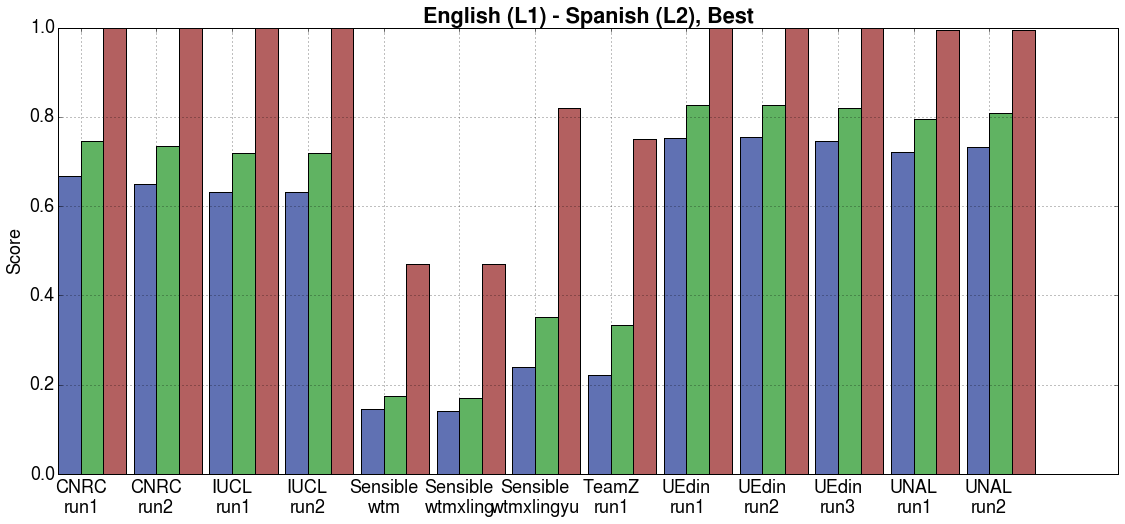
\includegraphics[width=16cm]{en-es-best-2.png}}
\noindent\makebox[\textwidth][c]{%
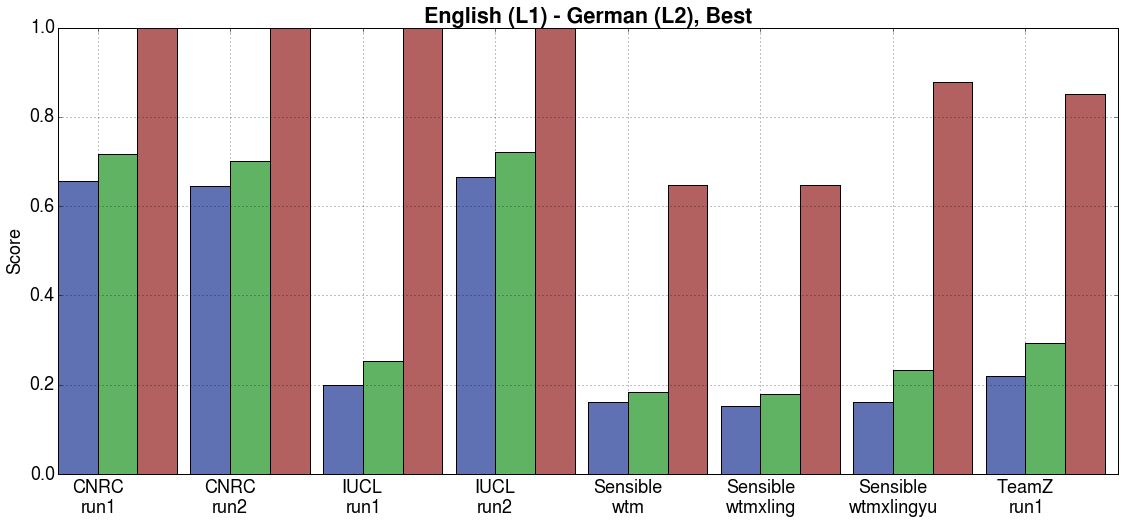
\includegraphics[width=16cm]{en-de-best-2.png}}
\noindent\makebox[\textwidth][c]{%
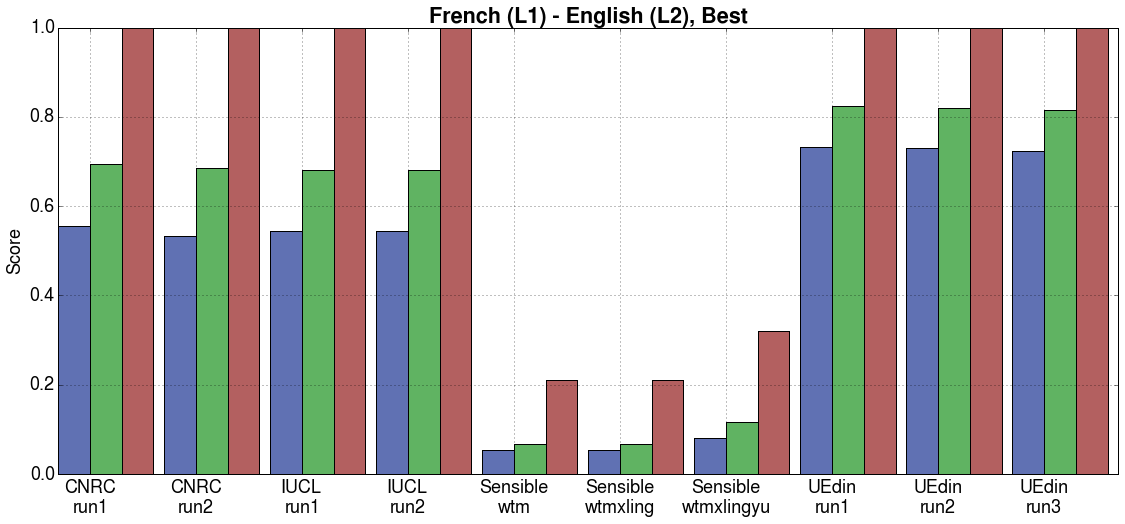
\includegraphics[width=16cm]{fr-en-best-2.png}}
\caption{English to Spanish (top), English to German (middle) and French to English (bottom). The three bars, left-to-right, represent Accuracy (blue), Word Accuracy (green) and Recall (red).}
\label{fig:graphs}
\end{figure*}

\section{Discussion}

We did not specify any training data for the task. The advantage of this is
that participants were free to build a wider variety of systems from various
sources, rather than introducing a bias towards for instances statistical
systems. The disadvantage, however, is that a comparison of the various systems
does not yield conclusive results regarding the merit of their methodologies.
Discrepancies might at least be partly due to differences in training data, as
it is generally well understood in MT that more training data improves results.
The baselines various participants describe in their system papers provide more
insight to the merit of their approaches than a comparison between them.

In the creation of the test set, we aimed to mimic intermediate to high-level
language learners. We also aimed at a fair distribution of different
part-of-speech categories and phrasal length. The difficulty of the task
differs between language pairs, though not intentionally so. We observe that
the Dutch-English set is the hardest and the Spanish-English is the easiest in
the task. One of the participants implicitly observes this through measurement
of the number of Out-of-Vocabulary words \citep{CNRC}. This implies that when
comparing system performance between different language pairs, one can not
simply ascribe a lower result to a system having more difficulty with said
language pair. This could rather be an intrinsic property of the test set or
the distance between the languages.

Distance in syntactic structure between languages also defines the limits of
this task. During composition of the test set it became clear that backing off
to L1 was not always possible when syntax diverged to much. An example of this
is separable verbs in Dutch and German. Consider the German sentence \emph{``Er
\textbf{ruft} seine Mutter \textbf{an}''} (translation: \emph{``He
\textbf{calls} his mother''}). Imagine a German language learner wanting to
compose such a sentence but wanting to fall back to English for the verb
\emph{``to call''}, which would translate to German as \emph{``anrufen''}. The
possible input sentence may still be easy to construe: \emph{``Er
\textbf{calls} seine Mutter''}, but the solution to this problem would require
insertion at two different points, whereas the task currently only deals with a
substitution of a single fragment. The reverse is arguably even more complex
and may stray too far from what a language learner may do. Consider an English
language learner wanting to fall back to her native German, struggling with the
English translation for \emph{``anrufen''}. She may compose a sentence such as
\emph{``He \textbf{ruft} his mother \textbf{an}''}, which would require
translating two dependent fragments into one.

We already have interesting examples in the gold standard, such as example (b),
showing syntactic word-order changes confined to a single fragment.

\begin{examples}
\footnotesize
%iris voorbeeld waar en-nl woordvolgende wisselt
\item[(b)] \textbf{Input:} I always wanted \textbf{iemand te zijn} , but now I realize I should have been more specific.\\
\textbf{Reference:} I always wanted \textbf{to be somebody} , but now I realize I should have been more specific.\\
\textbf{Participant output (aggregated):} to be a person; it to be; someone to his; to be somebody; person to be; someone to; someone to be; to be anybody; to anyone; to be someone; a person to have any; to be someone else
\end{examples}

Another question we can ask, but have not investigated, is whether a language
learner would insert the proper morphosyntactic form of an L1 word given the L2
context, or whether she may be inclined to fall back to a normal form such as
an infinitive. Especially in the above case of separable verbs someone may be
more inclined to circumvent the double fragments and provide the input:
\emph{``He \textbf{anrufen} his mother``}, but in simpler cases the same issue
arises as well. Consider an English learner falling back to her native
Croatian, a Slavic language which heavily declines nouns. If she did not know
the English word \emph{``book''} and wanted to write \emph{``He gave the book
to him''}, she could use either the Croatian word \emph{``knjigu''} in its
accusative declension or fall back to the normal form \emph{``knjiga''}. A
proper writing assistant system would have to account for both options.

We can analyse which of the sentences in the test data participants struggled
with most. First we look at the number of sentences that produce an average
word accuracy of zero, measured per sentence over all systems and runs in the
out-of-five metric. This means no participant was close to the correct output.
There were 6 such sentences in English-Spanish, 17 in English-German, 6 in
French-English, and 32 in Dutch-English.

%discuss user errors:
A particularly difficult context from the Spanish set is when a subjunctive
verb form was required, but an indicative verb form was submitted by the
systems, such as in the sentence: \emph{``Espero que los frenos del coche
\textbf{funcionen} bien.''}. Though this may be deduced from context (the word
\emph{``Espero''}, expressing hope yet doubt, being key here), it is often
subtle and hard to capture. Another problematic case that recurs in the German
and Dutch data sets is compound nouns. The English fragment \emph{``work
motivation''} should translate into the German compound
\emph{``Arbeitsmotivation''} or \emph{``Arbeitsmoral''}, yet participants were
not able to find the actual compound noun. Beside compound nouns, other less
frequent multi-word expressions are also amongst the difficult cases. Sparsity
or complete absence in training data of these expressions is why systems
struggle here.


%iris ik vind deze gewoon mooi:
%\textbf{Input:} Miami Beach is where neon {\emph naartoe gaat om te sterven }.\\
%\textbf{Reference:} Miami Beach is where neon \emph{ goes to die} .\\
%\textbf{Different participant output:} goes to die; is going to die; is going to go to die; goes of death; is going of death; go to die; are going to die; is being sent to of death; are allocated is of death; is heading of death; going to die; 's going to lead to die\\


Another point of discussion is the fact that we enriched the test set by adding
previously unavailable alternative translations from an aggregated pool of
system output. This might draw criticism for possibly introducing a bias, also
considering the fact that the decision to include a particular alternative for
a given context is not always straightforward and at times subjective. We,
however, contend that this is the best way to ensure that valid system output
is not discarded and reduce the number of false negatives. The effect of this
measure has been an increase in (word) accuracy for all systems, without
significant impact on ranking.


\begin{figure*}[bth] %cheating to get the figure at the same page
\noindent\makebox[\textwidth][c]{%
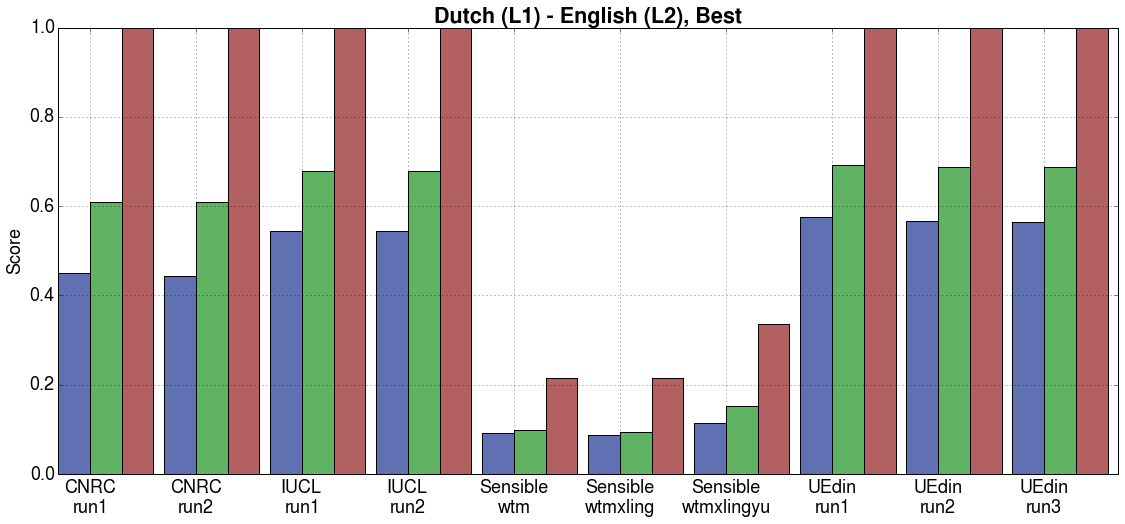
\includegraphics[width=16cm]{nl-en-best-2.png}
}
\caption{Dutch to English.}
\label{fig:graphs2}
\end{figure*}

\section{Conclusion}

In this SemEval task we showed that systems can translate L1 fragments in an L2
context, a task that finds application in computer-assisted translation and
computer-assisted language learning. The localised translation of a fragment in
a cross-lingual context makes it a novel task in the field. Though the task has
its limits, we argue for its practical application in a language-learning
setting: as a writing assistant and dictionary replacement. Six contestants
participated in the task, and used an ensemble of techniques from Statistical
Machine Translation and Word Sense Disambiguation. Most of the task organizers'
time went into manually establishing a gold standard based on a wide variety of
sources, most aimed at language learners, for each of the four language pairs
in the task. We have been positively surprised by the good results of the
highest ranking systems.

\section{Acknowledgements}

We would like to thank Andreu van Hooft and Sarah Schulz for their manual
correction work, and Sean Banville, Geert Joris, Bernard De Clerck, Rogier
Crijns, Adriane Boyd, Detmar Meurers, Guillermo Sanz Gallego and Nils Smeuninx
for helping us with the data collection.

\lstset{language=xml,basicstyle=\ttfamily\small,inputencoding=utf8,extendedchars=true,literate={ú}{{\'u}}1 {á}{{\'a}}1 {ã}{{\~a}}1 {é}{{\'e}}1 }


\title{The Role of Context Information in L2 Translation Assistance}



In this chapter we conclude the work started in
Chapters~\ref{chap:colibritapilot} and \ref{chap:semeval2014task5}, and
investigate to what extent L2 context information can aid the translation of L1
fragments in an L2 context, and what techniques are most suitable. We focus on
two approaches: the classifier-based approach from
Chapter~\ref{chap:colibritapilot}, and one rooted in Statistical
Machine Translation.  Various mixtures between the two are investigated. We
explicitly investigate the the role of context information (in L2) and of the
L2 language model. We test the incorporation of memory-based classifiers, as it
is proven method in Word Sense Dismambiguation, as a means of better
disambiguating the L1 fragments.  We find Statistical Machine Translation to be
the most adequate solution to the problem, and show how it can be applied with
a cross-lingual context. Integrating classifiers in such a framework has
little merit, as there is considerable overlap with the functioning of the L2
language model.

\textsc{This chapter is based on: } \emph{The Role of Context Information in L2 Translation Assistance}

  
\section{Introduction}

In this study we test and compare two approaches to translate L1 fragments in
an L2 context, focussing on the use of memory-based classifiers to disambiguate
the L1 fragments using their L2 context information. The first approach is
purely classifier-based, whereas the second integrates classifiers in
phrase-based statistical machine translation. This latter approach enhances the
translation model component by taking context directly into account in
translation. 

The MT-integrated system described is described in Section~\ref{sec:mtbased}.
The pure classifier-based approach is mainly described in
Chapter~\ref{sec:colibritapilot}, we offer a recap in
Section~\ref{sec:classifierbased}. In the present study, it will be re-evaluated on the
data from our SemEval-2014 ``L2 Translation Assistant'' task
(Chapter~\ref{chap:semeval2014task5}, which provides a
a representative test set where none existed yet.

Section~\ref{previous} briefly summarises the most important findings from the
participants in the SemEval task, and what we have learned from it.  In
Section~\ref{methodology} we describe the data used for our experiments, as
well as the evaluation metrics used throughout the study. We discuss the
results of our experiments and formulate our conclusions in
Section~\ref{discuss}.

\section{SemEval Results} %TODO: shorten further, remove redundancy
\label{previous}
\label{sec:participants}

Six participants took part in the SemEval task by writing a translation
assistance system. This provides an interesting basis for comparison,
although direct comparison is complicated by the fact that the SemEval task did
not specify a training set. 

The study by SemEval participant \cite{CNRC} shows that a solution based on
standard Phrase-based Statistical Machine Translation is viable strategy of
tackling the L2 Translation Assistant task. They present a clean and vanilla
approach using their Portage decoder \citep{PORTAGE}, in which the L2 context
is explicitly passed as context, and the remaining L1 fragment is translated,
yielding a full sentence translation in L2. They score well in the SemEval
task, finishing in second or third place for all language pairs.

The best-performing system \citep{UEDIN}, finishing in first place for
the three language pairs in which it participated, follows a very similar
strategy, using the Moses MT decoder \citep{MOSES}. They pass the
entire sentence, i.e the L1 fragment in the L2 context, to the
decoder. The L2 context is specifically marked to be left untouched by
the decoder, using XML syntax supported by Moses. In this XML format,
the L2 context has its translations explicitly passed, and reordering
walls prevent the decoder from changing the word order, leaving only
the L1 fragment to be translated. This method was proposed
earlier in a predecessor of Moses \citep{Cabezas+05}. Consider
Example~\ref{ex:xml} showing the XML input example from \cite{UEDIN},
in which L2 is English and L1 is French:

\begin{exmp}
\label{ex:xml}
\begin{lstlisting}
<wall/>les manifesteurs<wall/>
<np translation="want">want</np><wall/>
<np translation="to">to</np><wall/>
<np translation="replace">replace</np><wall/>
<np translation="the">the</np><wall/>
<np translation="government">government</np><wall/>
<np translation=".">.</np><wall/>
\end{lstlisting}
%\caption{Moses input fragment in XML with translation for L2 context specifically given and reordering walls inserted, from \cite{UEDIN}.}
\end{exmp}

They show that this results in a considerable improvement over a baseline that
translates just the L1 fragment without any L2 context. In fact, we will see
later that this simple and intuitive method outperforms the 
classifier-based method from the pilot study, which does not directly invoke
an MT decoder. We will therefore expand our system using this method, and
extend it to take classifier output into account.

The remaining participants in the SemEval task do not use a
traditional MT decoder. Nevertheless, two of them achieve good scores.
\cite{IUCL}, who finish first for the English -- German pair, build
their own distinct log-linear model for the task, which combines
various information sources. Amongst the features in this model are
the translation probability and inverse translation probability,
directly taken from a phrase-translation table built using GIZA++
\citep{GIZA} and the Moses training scripts for phrase extraction
using the {\em grow-diag-final-and}\/ algorithm.

\cite{UNAL} use a classifier-based approach using Timbl \citep{TIMBL},
which is the same memory-based classifier as used in the pilot study,
as well as this present study. \cite{UNAL} hypothesize that the
relevance of the context words for determining a correct translation
is proportional to their syntactic relatedness to the target, rather
than their physical closeness in the sentence, a hypothesis also
investigated by \cite{Haque+11}. \cite{UNAL} run a dependency parser
on the data and use syntax as a feature selector rather than as a
feature itself. This results in a feature vector of relevant
words. However, they do not find improvement over their baseline using
local context information (2 words left, 2 words right) using this
method. This team participated only on the English -- Spanish pair,
but they do rank second. This reconfirms that there is merit in
classifier-based approaches.

The SemEval participants employ various different methods to relate to
the L2 context. \cite{CNRC} fully rely on the L2 Language Model,
\cite{UEDIN} introduces an additional context-similarity feature to
the log-linear equation at the heart of the decoder. They derive this
from a phrase pair topic model, and find this improves results.


\section{Methodology}
\label{methodology}

From the systems participating in the SemEval task we observe that Statistical
Machine Translation (SMT) techniques as well as classifier-based techniques are
capable of achieving good performance on the L2 Translation Assistant Task. The
various participants' systems can not be readily compared and assessed on the
merit of their approach, as training data and training methods differ. In this
study, we do have two comparable systems. We assess the impact of L2 context
information in a purely classifier-based system, and in a MT-based hybrid system
enhanced with similar classifiers. 

It has to be strongly emphasised that our focus is on text data in its surface form,
without any further associated linguistic information requiring external
language-specific resources, such as taggers or parsers. We want to assess the
efficacy of context information in its purest unmodified form as we aim for an
approach that is as language-independent as possible. The inclusion of certain
well-chosen linguistic features may likely achieve better results than our
approach. However, results from both \cite{UNAL} as well as \cite{IUCL} already
show that intuitively promising linguistically-informed features, dependency
features in this case, do not always lead to an improvement over local lexical
context information. Unlike those studies, we do not introduce a new
linguistically-informed feature, but we deliberately constrain ourselves to
assess whether the context as-is has merit in the translation task.

This approach is motivated by the fact that local context information of
surface forms proves a powerful cue in word sense disambiguation, a field of
research with notable similarities to the task at hand. Often fairly small
window sizes lead to the best results, as shown in Chapter~\ref{chap:clwsd}.
These good results were achieved using memory-based classifiers. We therefore
bring these techniques to the present issue of translating L1 fragments in an
L2 context, and investigate their efficacy.

To test whether we do not constrain ourselves too much with mere local context
features, we also conduct a small experiment with global context features, i.e.
identifying powerful keywords for a given translation from the entire
sentential context.

These two aforementioned WSD studies were performed in the context of the
SemEval Cross-Lingual Word-Sense Disambiguation task in two past instances of
SemEval \citep{WSD,Lefever2013}, and emerged as the winning system for that
task. These studies do find a beneficial effect including lemmas as
part of the local context information, whereas part-of-speech tags do not
improve results. 

\subsection{Data \& Software}

The training data for our translation model is composed of two major
parallel corpora joined together: Europarl v7 \citep{EUROPARL} and
OpenSubtitles 2012\footnote{http://www.opensubtitles.org}
\citep{OPUS2012}.  Table~\ref{tab:datasize} lists the size of these
corpora. 

\begin{table}[htb]
\begin{center}
\caption{Corpora sizes for all of the language pairs}
\label{tab:datasize}
\begin{tabular}{|l|l|r|}
\hline
L1 & L2 & Sentences \\
\hline
English & Spanish &  41,797,582 \\
English & German & 7,542,070 \\
French & English & 24,862,173 \\
Dutch & English & 26,347,136 \\
\hline
\end{tabular}
\end{center}
\end{table}

For all our systems, a phrase-translation table was built using the Moses
scripts, first invoking GIZA$++$ for word-alignment and subsequently performing
phrase-extraction using the \emph{grow-diag-final} algorithm. This
phrase-translation table serves as the foundation for building the classifiers,
as shall be explained in Section~\ref{sec:classifierbased}.

An L2 language model is generated using SRILM \citep{SRILM}. We use a trigram
language model with Kneser-Ney smoothing. The model is trained on the L2 side
of the parallel corpus. It plays an essential role in the MT-based hybrid system,
and can be enabled as an extra component in the classifier-based system. 

Both systems are implemented in our software package
\emph{colibrita}.\footnote{\emph{colibrita} is written in Python 3, is open source
  (GPL v.3), and available from
  \url{http://github.com/proycon/colibrita/}. Version tag
  \texttt{0.3.1} is representative for the version used in this
  research and includes scripts for running the experiments.
  Colibita dependents on \emph{colibri-core} and \emph{colibri-mt}, both obtainable from the same github source, version tag \texttt{colibrita-v0.3.1} represents the state at
  the time of research.
  }
All input and output data of our experiments is also available for
download. \footnote{Freely available through Academic Torrents: \url{http://academictorrents.com/details/ab6e61059b7f7879e027ca33fb0f9e82980cd855} }

\subsection{Evaluation}

The translation results are automatically evaluated against multiple human
reference translations in the SemEval test set from
Chapter~\ref{chap:semeval2014task5}. This test set explicitly takes alternatives
into account; the evaluation metrics do so too. The evaluation
metrics\footnote{Although common in MT research, we do not report on the BLEU \citep{BLEU} score. In
Chapter~\ref{chap:colibritapilot} we already ascertained that this measure correlates well with
our task-specific accuracy metrics, but it has little added value because most of the sentence is already
translated and therefore BLEU scores are unnaturally high.} have been shown in
Section~\ref{sec:semeval2015task5evaluation}. When matching with multiple reference translations, the highest
score is taken. 

\section{Classifier-based System}

\label{sec:classifierbased}

\subsection{System Description}

The classifier-based system is the system as described in
Chapter~\ref{chap:colibritapilot}. Recall that we employ classifier experts; a
separate classifier for each possible input phrase, i.e. word or $n$-gram, and
each classifier thus specialises in the translation of a single word or phrase,
in all of the distinct contexts and with all of the different translations that
it is seen with in the training data. In this section we recap how this system
works, and add some details on its improved implementation and application in
the present study.

Classifier experts are built for each L1 phrase that has multiple L2
translation candidates, i.e. are ambiguous, provided that the phrase pair
exceeds a certain threshold. This threshold must be met by the product of the
translation probability and its inverse, i.e. $P(source|target) \cdot
P(target|source)$.  In our experiments here, the threshold is set to $0.0001$
to prune the worst candidates and keep file sizes and memory consumption
manageable. Recall from Chapter~\ref{chap:colibritapilot} that phrases that are
unambiguous (in the training data) are translated directly by a simple mapping
table.

Given the phrase-translation table we use for training, the task of collecting
the necessary training data for classification requires finding all positions
in the corpus where the L1 and L2 phrase from each of the phrase pairs occur.
When we have these positions we can extract the context information we need for
the classifiers' feature vectors.  This position data, however, is not present
in the phrase-translation table itself.  We therefore proceed to construct an
index of all phrases on either side of the parallel corpus, including only
those that occur in the phrase-translation table. This is done using
\emph{colibri-core}\footnote{\url{https://github.com/proycon/colibri-core}},
introduced in Chapter~\ref{chap:coco}, and constitutes our forward index. 
%We use it to look up the positions for each phrase pair in the phrase
%translation table. 
If both the source phrase and target phrase are found in a sentence pair, we
assume we found a translation instance. This is an assumption because at this
stage we do not have the actual word alignments loaded. If multiple translation
candidates are present in the L2 sentence, the one with the highest probability
according to the phrase table takes precedence. Our system could be improved by
consulting the actual GIZA++ word alignments at this stage.

In addition to this forward index, \emph{colibri-core} is also used to build a reverse
index, i.e a mapping of positions to words, only for the L2 side of the parallel
corpus in this case. This allows us to quickly extract local context
information in the form of $m$ words to the left and $n$ words to the right.
This is done using \emph{colibri-mt}\footnote{\url{https://github.com/proycon/colibri-mt}}.
Each instance found is added to the memory of the classifier expert dedicated
to the L1 phrase, in which the L2 context information constitutes the feature
vector, and L2 phrase is the class label. This procedure potentially generates a large
number of classifiers, which we constrain drastically by only generating those
that will be actually needed in the test stage.
% how many exactly?
When the memories are constructed for all, the actual
training begins and proceeds independently for each of the classifier experts.
For the variant of the IB1 algorithm as implemented in Timbl, this entails the computation of
feature weights for each of the local context features.


%Why not a simpler, less memory-intensive, approach iterating over GIZA++ word alignments?
%   - current approach is faster (at the expense of memory)
%   - we iterate per phrase-pair rather than per training sentence, allowing us to discard phrase-pairs without ambiguity, or not meeting a threshold
%   - current approach supports multiple factors

The test phase is straightforward. Each test L1 fragment in L2 context
is explicitly marked in the SemEval test data. Per sentence, we check
if we have a classifier for the marked fragment, and if so, we extract
the context features and pass it to the classifier. This produces a
translation, or rather, a probability distribution of translation
options. Prior to checking whether a classifier is present, we first
check if the L1 fragment is in the direct mapping table established
for unambiguous translations, and resort to that instead if found. It
is possible that a certain fragment has not been seen during training
and is neither in the simple mapping table, nor do we have a
classifier for it. In such cases, we are unable to translate the
fragment. This is one of the main weaknesses of this classifier-based
approach we later attempt to mitigate using an MT approach.

Recall that a statistical language model is implemented as an optional component
of the classifier-based system. We also use it as a baseline to compare our
system to Chapter~\ref{chap:colibritapilot}}.

Various parts of the search and classification process can in theory be
parametrised with weights. We follow the practices established in
Chapter~\ref{chap:colibritapilot}: We assign equal importance to translation
model and language model. We use default parameters\footnote{$k=1$, weighted
    overlap (\texttt{-m O}), and weighted using GainRatio (\texttt{-w gr}).
Note that $k=1$ in Timbl refers to the neigbours at the shortest distance, it
may still contain multiple instances if they are at the same distance.} for
Timbl, the $k$-Nearest Neighbour classifier, as parameter optimisation at this
stage has been shown not to yield a positive impact and prone to overfitting in
a comparable WSD setting, as shown in Chapter~\ref{chap:clwsd}. Whereas we
conducted automatic feature selection per classifier expert in
Chapter~\ref{chap:colibritapilot}, and found marginal
improvements with it, we omit this in the present chapster to reduce
experimental complexity. We deal with larger data now and it quickly becomes
computationally prohibitive.

\subsection{Experiments and Results}

We conducted a series of experiments to test whether the conclusions from
Chapter~\ref{chap:colibritapilot} hold on the more representative test set of
the SemEval Task. 

Two baselines were created. The first is a ``most likely fragment'' baseline
(MLF). This baseline does not use any context information and merely selects
the most frequent translation option for a given L1 fragment, according to the
phrase-translation table. It is used as a control for our context-informed
experiments, which in the pilot study surpassed this uninformed baseline, and
we hypothesise the same will occur with the improved test set.

A second baseline is constructed by weighing the probabilities from the
translation table directly with the aforementioned L2 language model (LM). This
effectively adds an LM component to the MLF baseline. This LM baseline allows
the comparison of classification through L1 fragments in an L2 context, with a
more traditional form of context modelling (i.e. target language modelling) as is
also customary in SMT decoders. The computation of the baseline proceeds as in
Equation~\ref{eq:LM}, with $score_T$ representing the normalised $p(t|s)$ score
from the phrase-translation table rather than the classifier.


We experimented with several configurations for the local context window. Starting
with one word left, one word right, up to three words left and right. We also
included an asymmetric configuration of two words to the left and one word to
the right. Omitting right context alltogether was already discarded in the pilot study.

Tables \ref{tab:resultsclassifier12} and \ref{tab:resultsclassifier34} show the
results of these experiments, for each of the four language pairs in the
SemEval task.  Statistical significance was computed on the Word Accuracy
metric, using the paired t-test, an asterisk indicates significance with respect to the
MLF baseline, and a $\ddagger$ indicates significance with respect to the LM baseline, both at $p < 0.05$.

\begin{table}[htb]
\begin{center}
\caption{Results of classifier-based experiments for English -- Spanish (left) and English -- German (right)}
\label{tab:resultsclassifier12}
\begin{tabular}{|l|rr|}
%generated at 2014-10-15 16:19 in /home/proycon/exp/expcolibrita/semeval3/en-es
%recall: 0.9538
\hline
System & Accuracy & W.Acc. \\%&  BLEU\\
\hline
MLF baseline & 0.544 & 0.651 \\%&  0.8737 \\
LM baseline & 0.643 & 0.720$*$ \\%&  0.9112 \\
\hline
l1r1 & 0.615 & 0.707$*$  \\% &  0.8983 \\
l1r1-lm & 0.651 & 0.736$*$ \\%&  0.9133 \\
l2r1 & 0.629 & 0.717$*$   \\%0.8991 \\
l2r1-lm & \textbf{0.657} & \textbf{0.742}$*\ddagger$ \\%&  \textbf{0.9135} \\
l2r2 & 0.628 & 0.722$*$ \\%&  0.9005 \\
l2r2-lm & 0.655 & 0.739$*$ \\%&  0.913 \\
l3r3 & 0.627 & 0.715$*$ \\%&  0.8992 \\
l3r3-lm & 0.649 & 0.729$*$ \\%& 0.9104 \\
\hline
\end{tabular}
\begin{tabular}{|l|rr|}
%generated at 2014-10-15 16:20 in /home/proycon/exp/expcolibrita/semeval3/en-de
%recall: 0.9459 
\hline
System & Accuracy & W.Acc. \\%& BLEU\\
\hline
MLF baseline & 0.571 & 0.627 \\%& 0.8756 \\
LM baseline & 0.605 & 0.657 \\%&  \textbf{0.8929} \\ %not significant! p==0.138430197902 !!
\hline
l1r1 & 0.617 & 0.672 \\%&  0.8884 \\
l1r1-lm & 0.603 & 0.656 \\%&  0.8894 \\
l2r1 & \textbf{0.635} & \textbf{0.690}$*$ \\%&  0.8915 \\
l2r1-lm & 0.613 & 0.665 \\%&  0.8927 \\
l2r2 & 0.625 & 0.681$*$ \\%&  0.8896 \\
l2r2-lm & 0.611 & 0.664 \\%&  0.8924 \\
l3r3 & 0.620 & 0.672$*$\\% &  0.8871 \\
l3r3-lm & 0.615 & 0.667$*$ \\%&  0.8913 \\
\hline
\end{tabular}
\end{center}
\end{table}



\begin{table}[htb]
\begin{center}
\caption{Results of classifier-based experiments for French -- English (left) and Dutch -- English (right)}
\label{tab:resultsclassifier34}
\begin{tabular}{|l|rr|}
%generated at 2014-10-15 16:22 in /home/proycon/exp/expcolibrita/semeval3/fr-en
%recall: 0.8222 
\hline
System & Accuracy & W.Acc. \\%& BLEU\\
\hline
MLF baseline & \textbf{0.519} & \textbf{0.614} \\%& 0.9159 \\
LM baseline & 0.507 & 0.596 \\%&  0.9195 \\ #%not significant (p=0.23)
\hline
%nothing is significant here!
l1r1 & 0.503 & 0.603 \\%&  0.9169 \\
l1r1-lm & 0.511 & 0.604 \\%&  \textbf{0.9201} \\
l2r1 & 0.503 & 0.601 \\%&  0.9163 \\
l2r1-lm & 0.511 & 0.604 \\%&  0.9198 \\
l2r2 & 0.493 & 0.595 \\%&  0.9146 \\
l2r2-lm & 0.503 & 0.598 \\%&  0.9178 \\
l3r3 & 0.499 & 0.600 \\%&  0.9155 \\
l3r3-lm & 0.503 & 0.598 \\%&  0.917 \\
\hline
\end{tabular}
\begin{tabular}{|l|rr|}
%generated at 2014-10-15 16:22 in /home/proycon/exp/expcolibrita/semeval3/nl-en
%recall: 0.6511 
\hline
System & Accuracy & W.Acc. \\%& BLEU\\
\hline
MLF baseline & 0.419 & 0.480 \\%& 0.921 \\
LM baseline & 0.370 & 0.445$*$ \\%&  0.9183 \\
\hline
l1r1 & \textbf{0.437} & 0.496$\ddagger$ \\%&  \textbf{0.9232} \\
l1r1-lm & 0.386 & 0.460$\ddagger$ \\%&  0.9197 \\
l2r1 & 0.435 & \textbf{0.497}$\ddagger$ \\%&  0.923 \\
l2r1-lm & 0.386 & 0.461$\ddagger$ \\%&  0.9198 \\
l2r2 & 0.431 & 0.495$\ddagger$ \\%&  0.9224 \\
l2r2-lm & 0.384 & 0.458 \\%&  0.9192 \\
l3r3 & 0.419 & 0.485$\ddagger$ \\%&  0.9211 \\
l3r3-lm & 0.378 & 0.454$*$ \\%&  0.9184 \\
\hline
\end{tabular}
\end{center}
\end{table}

The main conclusion from the pilot study was that classifiers informed by
simple local context features outperformed both the non-context-informed
baseline as well as the LM baseline. We see that this former conclusion holds
for two out of four language pairs: English -- Spanish and English -- German.
For the remaining two language pairs, it is either below baseline or fails to
pass significance tests.\footnote{All mentions of significance in this chapter are
statistically backed using a paired t-test with $p<0.05$} This puts the
conclusion from the pilot study in question.  Similarly, improvement over LM
baseline is only observed in two out for four language pairs.

The results for English -- Spanish support the idea of memory-based classifiers
as a means to solve this task the strongest. We first perceive a significant
gain in accuracy for the LM Baseline, compared to the MLF baseline, and all
classifier-based systems again consistently improve over the MLF baseline.  For
improvement over the LM baseline we only have one system, the best one,  which passes the
significance test. The pilot study concluded that the language model and
classifiers were able to complement each other, despite significant overlap in
what they model. We do see that the best system for English -- Spanish is the
system that combines classifiers and adds a language model as well. The highest
score is achieved for the asymmetric configuration with two words to the left,
and one word to the right.

The English -- German pair reconfirms the classifier's ability to beat the
non-context-informed baseline, but adding a language model component proves to have little
added value here. The LM baseline does not significantly improve upon the MLF
baseline either.

For the last two language pairs, both translating to English, the classifiers
make no significant impact over the MLF baseline whatsoever. We speculate that
morphological richness may be a factor here: when translating from a
morphologically simpler language to a morphologically richer\footnote{i.e.
distinguishing a higher diversity of surface forms for a given lemma} language,
such as English to Spanish and English to German, the classifiers have a bigger
role to perform and may prove beneficial. That being said, we can not jump to
this conclusion too quickly, as the different sets do not just differ in
language pair, but despite our best efforts to deliver a balanced test, also
differ in difficulty, the English-Spanish set being the easier one, and the
Dutch-English set being the hardest.

We do not at all observe a strong effect of the language model being
complementary with the classifier system, as was demonstrated in the pilot
study. When adding an LM component to our classifier-based system, we see a
positive impact over both MLF and LM baseline for only the English -- Spanish
language pair.  Although the classifiers model L1 fragments in and L2 context,
and the LM models only L2 without integrating the translation step, these are
different methods to the same end, and the models will inevitably overlap to a
degree, especially if they model roughly the same size of local context.

%too speculative:
%Here too speculate this could be caused by Spanish being
%morphologically richer than English and agreements in gender and number in noun
%phrases being fairly easy to resolve in Spanish by a language model. The
%language model clearly has a much tougher task in German, part of which we may
%attribute to the notion of grammatical case which typically is not easily
%derivable from a small local context. 

Regarding the size of the local context window, we see best performance for
small context sizes, with all of the winning scores in either \emph{l1r1} (one word to
the left, one word to the right) or \emph{l2r1} (two words to the left, one word to
the right). Results for \emph{l3r3} consistently show a performance drop. However, the
configurations are too similar to pass statistical significance tests.

\subsection{Additional experiments}

It may be argued that a trigram language model, as used in all our experiments,
has little to offer over classifiers that model roughly the same size of local
context window. We therefore conducted a small extra experiment for English --
German, \emph{l1r1}, with a 5-gram language model with Kneser-Ney smoothing. This does
not result in a significant improvement over \emph{l1r1-lm}, with a word accuracy of
$0.6587$, an absolute accuracy of $0.6052$, and does not significantly differ
from the \emph{l1r1} configuration either (without language model).  %, and a BLEU score of $0.891$, 

One of the main points of contention for this present study is our emphasis on
simple, and often even small, local context features. Intuitively, there is
great appeal in incorporating global context keywords, i.e. finding
high-frequency words in the whole sentential context that prove salient for a
given translation pair. These can be incorporated into the feature vector using
a bag-of-word configuration with binary values indicating presence of absence.
Surprisingly, our studies with memory-based classification in word sense
disambiguation in Chapter~\ref{clwsd} show that these global keywords do not
always have enough disambiguation power to beat local context. Our WSD2 system
on SemEval 2013 data (Section~\ref{sec:wsd2}) did not lead to an improvement
over local context, whereas our very similar and earlier UvT-WSD1 system on
SemEVal 2010 data (Section~\ref{sec:uvtwsd1}) did. We suspect this may be
attributed to increased sparsity due to the difference in data, as the systems
are as good as identical. We put this to the test again by once again
conducting an extra experiment using global context keywords in the same
fashion\cite{NgL96}. We find results significantly below our MLF baseline, with
a drop in accuracy and word accuracy to $0.4930$ and $0.5686$, respectively.

\section{MT-based hybrid System}
\label{sec:mtbased}

\subsection{Introduction}

During this research, thanks to insights from SemEval task
participants \cite{UEDIN} and \cite{CNRC}, it became apparent that we
could improve results by switching to an SMT-based system. We are not
parting from using classifiers to disambiguate L1 fragments in an L2
context to the proper L2 translation, but we are integrating these
classifiers in a full statistical machine translation framework,
analogous to \cite{Haque+11}. The idea is that SMT has no facilities to
explicitly model context, let alone cross-lingual context. The classifiers fill
this void and we aim to assess whether incorporating classifiers has merit.

\subsection{System Description}

The training and construction of the classifiers does not differ from the
classifier-based system. For the phrase-translation table we already used the
pipeline offered by SMT system Moses \citep{MOSES}, so that remains identical as
well.

The difference lies in the test phase, where we actually use the Moses
SMT decoder to do the job, rather than just invoking
classifiers. Moses cannot explicitly model context in its translation
model, so we still rely on the classifiers for that. In order to
integrate these classifiers into the decoder, we make use of Moses'
ability to read XML input in which translation for parts can be
explicitly provided. An example of such XML input was shown in
Example~\ref{ex:xml} in Section~\ref{sec:participants}.

Because we use Moses, we have an extra parameter tuning step to perform prior
to testing. We use Minimum Error Rate Training (MERT) \citep{MERT} to tune the
weights that drive the log-linear combination at the heart of the decoder,
determining precisely how much importance to give to the various scores of the
translation model, the language model, and other models. We tune our system on
data from the News Commentary corpus\footnote{Part of the WMT 2013 shared task
training data, \url{http://www.statmt.org/wmt13/translation-task.html}} for
three out of the four language pairs: English -- Spanish, English -- German and
French -- English. For Dutch -- English we have to resort to another corpus, a
collection of transcribed bilingual TED talks compiled for the IWSLT 2012
Evaluation
Campaign\footnote{\url{http://hltc.cs.ust.hk/iwslt/index.php/evaluation-campaign/ted-task.html}}. 
We use 10,000 sentence pairs for each. The choice for these corpora, as opposed
to a subset of Europarl or Opensubtitles, is motivated by our aim for more
generalisation.

When obtaining a test sentence in L2 with a marked fragment in L1, we first
pass the fragment through the classifier, if a classifier exists for the
fragment. The classifier outputs a distribution of translation
options, with associated confidence scores. We can pass multiple translation
options with associated probabilities to Moses with XML syntax, consider the
excerpt in Example~\ref{ex:xml2}, in which three translation options are
received from the classifier and passed to the Moses decoder using XML:

\begin{exmp}

\label{ex:xml2}
\begin{lstlisting}
<w translation="es">es</w><wall/>
<w translation="importante">importante</w><wall/>
<w translation="cuidarse">cuidarse</w><wall/>
<w translation="y">y</w><wall/>
<f translation="la única||la única forma||la única manera"
 prob="0.555556||0.333333||0.111111">the only way</f><wall/>
<w translation="es">es</w><wall/>
\end{lstlisting}
\end{exmp}

The Moses decoder now deals with the scores derived from the classifier, rather
than those from the phrase translation table, and is then mainly driven by
the language model, as the translations are fixed. 

The scores from the classifier are much coarser than those from the
phrase-translation table, as those in the phrase-translation table consist of
four components,\footnote{conditional probabililies $p(s|t)$, $p(t|s)$ and
corresponding lexical weights} and we are tweaking only a single component,
namely $p(t|s)$. As this would result in a skewed integration of classifier
scores, we implement a ``weighted'' method that performs part of the decoder's
log-linear equation, parametrised by the weights obtained from MERT, and passes
this weighted result to Moses using the XML syntax. This workaround is
necessary because the XML input method itself is limited and offers no
facilities to specify just a single component of the translation model.

To assess whether the information from our classifiers outperforms a baseline
without such classifiers, we establish a new MT-based baseline that does not
incorporate classifiers and just passes the fragment as-is for the decoder to
translate, as shown in Example~\ref{ex:xml3}:

\begin{exmp}
\label{ex:xml3}
\begin{lstlisting}
<w translation="es">es</w><wall/>
<w translation="importante">importante</w><wall/>
<w translation="cuidarse">cuidarse</w><wall/>
<w translation="y">y</w><wall/>
the only way<wall/>
<w translation="es">es</w><wall/>
\end{lstlisting}
\end{exmp}

From our experiments it becomes apparent that it is hard to surpass
this baseline. We therefore added another configuration that uses the
classifier output in a first-past-the-post fashion; if a classifier makes a
prediction that reaches a certain threshold, we use that classifier prediction,
otherwise we use Moses and do not pass it any information from the classifiers.
%This is an all-or-nothing approach on the other side of the spectrum, opposite to the
%subtle weighting approach.

In order to pass numerous test fragments to Moses at high speed, we run Moses
as a server, and use our software \emph{colibrita} to connect to it after
having classified each fragment.

\subsection{Experiments \& Results}

Tables \ref{tab:resultsmt12} and \ref{tab:resultsmt34} show the results of these experiments, for each of the
four language pairs in the SemEval task. The \emph{``mosescut''} configurations, refer
to the first-past-the-post approach, with the number indicating the threshold.
It is the coarsest form of integration. Next is the \emph{``moses''} configuration
which just passes the classifier score to the decoder. Last, \emph{``mosesweighted''}
is the most fine-grained form of integration and computes part of the
log-linear equation prior to passing it to the decoder. For reference we
 include the MLF baseline as well as the best scoring classifier-based system from the earlier tables.
Statistical significance was computed on the Word Accuracy
metric, using the paired t-test; an asterisk indicates significance with respect to the
MLF baseline, and a $\ddagger$ indicates significance with respect to the MT baseline, both at $p < 0.05$.


\begin{table}[htb]
\begin{center}
\caption{Results of MT-based experiments for English-Spanish (left) \& English-German (right)}
\label{tab:resultsmt12}
\begin{tabular}{|l|rr|}
%generated at 2014-10-15 16:19 in /home/proycon/exp/expcolibrita/semeval3/en-es
\hline
System & Accuracy & W.Acc. \\%& BLEU\\
\hline
MLF baseline & 0.544 & 0.651 \\%& 0.8737 \\ %recall: 0.9538 
MT baseline & 0.651 & 0.750$*$ \\% & 0.9069 \\ %recall: 1.0 
\hline
l2r1-lm & 0.657 & 0.742$*$ \\%& \textbf{0.9135} \\ %recall: 0.9538 
\hline
l1r1-moses & 0.625 & 0.736$*$ \\%& 0.874 \\
l1r1-mosescut0.7 & 0.657 & 0.761$*$ \\%& 0.9111 \\
%l1r1-mosescut0.8 & 0.6526 & 0.7563 & 0.9097 \\
%l1r1-mosescut0.9 & 0.6486 & 0.7531 & 0.9081 \\
l1r1-mosesweighted & 0.610 & 0.724$*$ \\%& 0.8672 \\
l2r1-moses & 0.647 & 0.755$*$ \\%& 0.885 \\
l2r1-mosescut0.7 & \textbf{0.669} & \textbf{0.774}$*\ddagger$ \\%& 0.9128 \\
%l2r1-mosescut0.8 & 0.6667 & 0.7715 & 0.9118 \\
%l2r1-mosescut0.9 & 0.6606 & 0.7663 & 0.9097 \\
l2r1-mosesweighted & 0.635 & 0.744$*$ \\%& 0.8795 \\
l2r2-moses & 0.649 & 0.756$*$ \\%& 0.8906 \\
%l2r2-mosescut0.7 & \textbf{0.6727} & 0.7733 & 0.9141 \\
%l2r2-mosescut0.8 & \textbf{0.6727} & 0.7731 & 0.9138 \\
%l2r2-mosescut0.9 & 0.6667 & 0.7679 & 0.9117 \\
%l2r2-mosesweighted & 0.6386 & 0.7464 & 0.8867 \\
l3r3-moses & 0.657 & 0.756$*$ \\%& 0.8979 \\
%l3r3-mosescut0.7 & \textbf{0.6727} & 0.7669 & \textbf{0.9144} \\
%l3r3-mosescut0.8 & \textbf{0.6727} & 0.7668 & 0.9138 \\
%l3r3-mosescut0.9 & 0.6647 & 0.7602 & 0.9109 \\
%l3r3-mosesweighted & 0.6586 & 0.7587 & 0.898 \\
\hline
\end{tabular}
\begin{tabular}{|l|rr|}
%generated at 2014-10-15 16:20 in /home/proycon/exp/expcolibrita/semeval3/en-de
\hline
System & Accuracy & W.Acc. \\%& BLEU\\
\hline
MLF baseline & 0.571 & 0.627 \\%& 0.8756 \\ %recall: 0.9459 
MT baseline & \textbf{0.689} & 0.745$*$ \\%& \textbf{0.9106} \\ %recall: 0.998 
\hline
l2r1 & 0.635 & 0.690 \\%& 0.8915 \\ %recall: 0.9459 
\hline
l1r1-moses & 0.603 & 0.672$*\ddagger$ \\%& 0.8793 \\ %recall: 0.998 
l1r1-mosescut0.7 & 0.681 & 0.739$*$ \\%& 0.9086 \\
%l1r1-mosescut0.8 & 0.6774 & 0.7357 & 0.9077 \\
%l1r1-mosescut0.9 & 0.6754 & 0.736 & 0.9071 \\
l1r1-mosesweighted & 0.569 & 0.651$\ddagger$ \\%& 0.8704 \\
l2r1-moses & 0.619 & 0.685$*\ddagger$ \\%& 0.8847 \\
l2r1-mosescut0.7 & \textbf{0.689} & \textbf{0.748}$*$ \\%& \textbf{0.9106} \\
%l2r1-mosescut0.8 & 0.6854 & 0.7444 & 0.9094 \\
%l2r1-mosescut0.9 & 0.6834 & 0.7437 & 0.9088 \\
l2r1-mosesweighted & 0.599 & 0.675$*\ddagger$ \\%& 0.8795 \\
l2r2-moses & 0.617 & 0.684$*\ddagger$ \\%& 0.8864 \\
l3r3-moses & 0.633 & 0.693$*\ddagger$ \\%& 0.8901 \\
\hline
\end{tabular}
\end{center}
\end{table}


\begin{table}[htb]
\begin{center}
\caption{Results of MT-based experiments for French-English (left) and Dutch-English (right)}
\label{tab:resultsmt34}
\begin{tabular}{|l|rr|}
%generated at 2014-10-15 16:22 in /home/proycon/exp/expcolibrita/semeval3/fr-en
\hline
System & Accuracy & W.Acc. \\%& BLEU\\
\hline
MLF baseline & 0.519 & 0.614 \\%& 0.9159 \\ %recall: 0.8222 
MT baseline & \textbf{0.620} & \textbf{0.742}$*$ \\%& \textbf{0.9425} \\ %recall: 0.998 
\hline
l1r1-lm & 0.511 & 0.604 \\%& 0.9201 \\%recall:0.8222 
\hline
l1r1-moses & 0.568 & 0.709$*\ddagger$ \\%& 0.9357 \\ %recall: 0.998 
l1r1-mosescut0.7 & 0.590 & 0.721$*\ddagger$ \\%& 0.938 \\
%l1r1-mosescut0.8 & 0.5899 & 0.721 & 0.938 \\
%l1r1-mosescut0.9 & 0.596 & 0.7251 & 0.9388 \\
l1r1-mosesweighted & 0.562 & 0.703$*\ddagger$ \\%& 0.9348 \\
l2r1-moses & 0.576 & 0.711$*\ddagger$ \\%& 0.9363 \\
l2r1-mosescut0.7 & 0.588 & 0.717$*\ddagger$ \\%& 0.9368 \\
%l2r1-mosescut0.8 & 0.5859 & 0.7163 & 0.9366 \\
%l2r1-mosescut0.9 & 0.5939 & 0.7214 & 0.9376 \\
l2r1-mosesweighted & 0.568 & 0.706$*\ddagger$ \\%& 0.9349 \\
l2r2-moses & 0.572 & 0.708$*\ddagger$ \\%& 0.9355 \\
%l2r2-mosescut0.7 & 0.5737 & 0.7054 & 0.9342 \\
%l2r2-mosescut0.8 & 0.5717 & 0.7044 & 0.934 \\
%l2r2-mosescut0.9 & 0.5798 & 0.7094 & 0.935 \\
%l2r2-mosesweighted & 0.5596 & 0.6974 & 0.9335 \\
l3r3-moses & 0.570 & 0.707$*\ddagger$ \\%& 0.9347 \\
%l3r3-mosescut0.7 & 0.5778 & 0.7086 & 0.9343 \\
%l3r3-mosescut0.8 & 0.5818 & 0.7126 & 0.9349 \\
%l3r3-mosescut0.9 & 0.5818 & 0.7126 & 0.9349 \\
%l3r3-mosesweighted & 0.5616 & 0.6986 & 0.9332 \\
\hline
\end{tabular}
\begin{tabular}{|l|rr|}
%generated at 2014-10-15 16:22 in /home/proycon/exp/expcolibrita/semeval3/nl-en
\hline
System & Accuracy & W.Acc \\%& BLEU\\
\hline
MLF baseline & 0.419 & 0.480 \\%& 0.921 \\%recall: 0.6511 
MT baseline & 0.534 & 0.677$*$ \\%& 0.9324 \\%recall: 1.0 
\hline
l2r1 & 0.435 & 0.497 \\%& 0.923 \\%recall: 0.6511 
\hline
l1r1-moses & 0.487 & 0.647$*\ddagger$ \\%& 0.9262 \\%recall: 1.0 
l1r1-mosescut0.7 & \textbf{0.548} & 0.686$*$ \\%& 0.9333 \\
%l1r1-mosescut0.8 & 0.5458 & 0.6851 & 0.9333 \\
%l1r1-mosescut0.9 & 0.5458 & 0.6851 & 0.9333 \\
l1r1-mosesweighted & 0.476 & 0.634$*\ddagger$ \\%& 0.9238 \\
l2r1-moses & 0.495 & 0.654$*\ddagger$ \\%& 0.9278 \\
l2r1-mosescut0.7 & \textbf{0.548} & \textbf{0.687}$*$ \\%& \textbf{0.9335} \\
%l2r1-mosescut0.8 & 0.5458 & 0.6865 & \textbf{0.9335} \\
%l2r1-mosescut0.9 & 0.5458 & 0.6865 & \textbf{0.9335} \\
l2r1-mosesweighted & 0.489 & 0.647$*\ddagger$ \\%& 0.9265 \\
l2r2-moses & 0.495 & 0.653$*\ddagger$ \\%& 0.928 \\
%l2r2-mosescut0.7 & 0.5419 & 0.6831 & 0.9326 \\
%l2r2-mosescut0.8 & 0.538 & 0.6816 & 0.9324 \\
%l2r2-mosescut0.9 & 0.5361 & 0.6797 & 0.9322 \\
%l2r2-mosesweighted & 0.4951 & 0.651 & 0.9271 \\
l3r3-moses & 0.497 & 0.654$*\ddagger$ \\%& 0.928 \\
%l3r3-mosescut0.7 & 0.5302 & 0.6728 & 0.9314 \\
%l3r3-mosescut0.8 & 0.5263 & 0.6713 & 0.9312 \\
%l3r3-mosescut0.9 & 0.5283 & 0.6733 & 0.9314 \\
%l3r3-mosesweighted & 0.4932 & 0.6481 & 0.927 \\
\hline
\end{tabular}
\end{center}
\end{table}

First, we observe that the MT baseline is considerably higher compared to the
classifier-based systems, and significantly higher than the MLF baseline on all
accounts. It surpasses all of the classifier-based scores consistently for all
language pairs. The MT baseline seems hard to beat, as both English -- German
and French -- English do not achieve results above baseline at all and the
positive impact for Dutch-English fails to pass the significance threshold.
Only English -- Spanish shows a clear positive impact of integrating context
information using classifiers, but only using the coarsest \emph{``mosescut''}
system, that places all bets on a single classifier prediction. The most
fine-tuned adjustment of the weights, \emph{``mosesweighted``}, consistently
underperforms, also for the higher configurations omitted from the tables.

We experimented with various different threshold values for the \emph{``mosescut''}
configuration, although these are omitted from the tables for brevity. We found
a threshold of $0.7$ to be performing amongst the best, for all language pairs.

This MT-based hybrid approach may seem to challenge our conclusion that classifiers
modelling context improve over a non-context informed baseline. But that is not
the case. The Moses baseline here is context-informed; it makes use of
a language model. We conducted a modified MT-baseline experiment on
English -- Spanish with the language model disabled. Word accuracy plummeted to
$0.44$, even below the MLF baseline. What is challenged, however, is the role
classifiers modelling source-side context can play when integrated in an SMT
decoder, and to what extent explicit modelling of context information is not
already implicitly captured by the language model. Still, however, we see
classifiers making a positive impact for two out of four language pairs.

%\begin{figure}
%\begin{center}
%  \includegraphics[width=100mm]{entropyaccuracy.png}
%  \caption{Scatter plot showing word accuracy as a function of the entropy of the distribution of
%  translation options, per test fragment. Measured on l2r1-moses for
%  English--Spanish. Linear regression was applied to show the general trend
%  ($R^2 = 0.09, p < 0.05$)}
%  \label{fig:entropyaccuracy}
%\end{center}
%\end{figure}
%Linear regression: r -0.301891558694 p 3.80580499306e-08 std_err 0.0271800621805

%In Figure~\ref{fig:entropyaccuracy}, we take a closer look at the performance
%of the classifiers by focussing on how multiple translation options are
%distributed in the classifiers and how this relates to the final word accuracy.
%We zoom in on the \emph{l2r1-moses} configuration for English--Spanish, i.e.
%the precursor to our best system, before the cut-off. For each instance, we
%measure the word accuracy as a function of the entropy of the distribution of
%translation options that is returned by the respective classifier expert for a
%test fragment.  We apply simple linear regression to
%illustrate the average trend, which illustrates, as expected, that word
%accuracy decreases as entropy grows.

\section{Discussion \& Conclusion}
\label{discuss}

%When comparing our results to the six participants in the SemEval task, we find that the winning system described in \cite{UEDIN}, remains at the top for all three language pairs it participated in. Our system comes in third for English-Spanish, first for English-German, second for 

Table~\ref{tab:comparison}, after \cite{SEMEVAL2014TASK5}, shows the
results of our best classifier-based and best MT-based hybrid
run\footnote{For French-English, the best run is the baseline system},
compared to the other six participants in the SemEval task.

\begin{table}[htb]
\begin{center}
\caption{Highest word accuracy per team, per language pair. The best score for each language-pair is marked in bold.}
\label{tab:comparison}
\begin{tabular}{|l|llll|}
\hline
Team & \textbf{en-es} & \textbf{en-de} & \textbf{fr-en} & \textbf{nl-en} \\ 
\hline
\textbf{MT-based} & $0.774$ (3$^{rd}$) & \textbf{0.748} (1$^{st}$) & $0.742$ (2$^{nd}$) & $0.687$ (2$^{nd}$) \\
\textbf{Classifier-based} & $0.742$ (4$^{th}$) & $0.690$ (4$^{th}$) & $0.610$ (4$^{th}$) & $0.497$ (4$^{th}$) \\ 
\hline
\textbf{CNRC} \citep{CNRC} & 0.745 & 0.717 & 0.694 & 0.610 \\
\textbf{IUCL} \citep{IUCL}  & 0.720 & 0.722 & 0.682 & 0.679 \\
\textbf{UEdin} \citep{UEDIN}  & \textbf{0.827} &  - & \textbf{0.824} & \textbf{0.692} \\
\textbf{UNAL} \citep{UNAL} & 0.809 & - & - & -  \\
\textbf{Sensible} \citep{SENSIBLE} & 0.351 & 0.233 & - & - \\
\textbf{TeamZ} \citep{TEAMZ} & 0.333 &  0.293 & - & -  \\
\hline
\end{tabular}
\end{center}
\end{table}

We have not been able to surpass the score of the winning system by
\cite{UEDIN}. What is different between our approaches? Rather than
incorporating classifiers modelling local context, \cite{UEDIN} add a context
similarity feature derived from a topic model that learns topic distributions
for phrase pairs, which improves performance over their baseline. Their
baseline is constructed in the same way as ours, except that it uses a
different parameter tuning method (the MIRA Tuning Algorithm) instead of MERT.
For English -- Spanish they do not surpass their own baseline, which attains an
even higher word accuracy of $0.839$. For French -- English their baseline
attains a score of $0.823$ and for Dutch -- English $0.686$, which is the score
our best MT-based hybrid system attains as well. The difference between our respective
baselines can be attributed to different training and tuning corpora.  Our
training data includes the OpenSubtitles corpus and is therefore much
larger, however, they train a larger language model on different data than the
translation model. This may likely account for better generalisation and better
scores. We confirm this by running an enriched MT-baseline experiment on
English -- Spanish with a substantially larger five-gram language
model\footnote{Trained on four corpora: Europarl, OpenSubtitles, MultiUN
(\url{http://www.euromatrixplus.net/multi-un/}) and NewsCrawl
(\url{http://www.statmt.org/wmt13/translation-task.html})}, and indeed
obtain scores that are higher than our standard MT-baseline.

This confirms the important role of the language model. We already saw
that for the language pairs translating from English, the language model
baseline beats the MLF baseline. Language modelling in the MT decoder is
clearly superior to our simpler implementation in the LM baseline, as we see
the MT baseline consistently above the LM baseline. We conclude that it is very
hard to attain results above this MT baseline, for an MT-based system enriched
with classifiers modelling just local context.

The role of the language model can also be assessed by inspecting the
weight it has received from the MERT parameter tuning algorithm. We express this
score relative to the weight of the $p(t|s)$ component of the translation
model\footnote{The $p(t|s)$ component of the translation model consistently has
a higher weight than the other (three) components} and obtain $1.12$ for
English -- Spanish, $1.37$ for English -- German, $0.62$ for French -- English
and $0.90$ for Dutch -- English. Overall, this means the language model weight
and translation model weight are fairly balanced and, as expected, both are
essential components. The language model carries more weight when
translating from English to Spanish or German, which we believe is due to the
target languages being morphologically richer and the stronger role the LM then
plays to select the proper morphological variant given the context.

Our best performing system is the first-past-the-post \emph{``mosescut''}
system, with slight but significant gains above the MT baseline for English --
Spanish. To gain some insight in the data, we take the English -- Spanish
output of the system \emph{l2r1-mosescut0.7} , and investigate the instances
where there is a difference with the MT baseline, which amounts to $70$
instances ($14\%$). The remaining instances were translated the same. We
decided to perform a limited\footnote{Single person, non-blind} human
evaluation of these seventy instances, to form an impression whether the
automatic evaluation metrics indeed correspond with human judgement, and
whether our system output can rightfully be considered to be better than the MT
baseline.  Out of the $70$ differing instances, the baseline was deemed to have
the better solution for $14$ of them, and the \emph{l2r1-mosescut0.7} system
had the better solution for $28$. The remaining $28$ instances were judged to
be equally good or equally bad. This is in line with the automatic evaluation
metrics but illustrates the very small margin we are working with.

Examples~\ref{ex:comp1}, \ref{ex:comp2} and \ref{ex:comp3} show a comparison of
some interesting output sentences where the role of context made a noticeable
difference. We also added the MLF baseline, which matches the MT baseline in a
lot of the $28$ cases where the mosescut system was found to perform better.

\begin{exmp}
\textbf{MLF baseline:} Le aconsejo este vino \textbf{rojo} de Argentina . \\
\textbf{MT baseline:} Le aconsejo este vino \textbf{rojo} de Argentina . \\
\textbf{l2r1-mosescut0.7:} Le aconsejo este vino \textbf{tinto} de Argentina .  \\
\label{ex:comp1}
\end{exmp}

\begin{exmp}
\textbf{MLF baseline:} El embajador \textbf{firmado} hoy el acuerdo . \\
\textbf{MT baseline:} El embajador \textbf{firmado} hoy el acuerdo . \\
\textbf{l2r1-mosescut0.7:} El embajador \textbf{ha firmado} hoy el acuerdo . \\
\label{ex:comp2}
\end{exmp}

\begin{exmp}
\textbf{MLF baseline:} En la actualidad se cuenta con la medicina \textbf{más avanzados} . \\
\textbf{MT baseline:} En la actualidad se cuenta con la medicina \textbf{más avanzados} . \\
\textbf{l2r1-mosescut0.7:} En la actualidad se cuenta con la medicina \textbf{más avanzada} . \\
\label{ex:comp3}
\end{exmp}

Still, we find examples of fragments where the wrong morpho-syntactic form was
selected. In the English -- German language pair, this selection is complicated
by the fact there are also cases in addition to gender, and number, which are
typically harder to resolve from a small local context. Example \ref{ex:comp4}
shows such an error where our system, as well as the baseline, selected a
dative form rather than the nominative:

\begin{exmp}
\textbf{Reference: } Ich habe einen guten Chef und \textbf{das Büro} liegt in der Nähe von meinem Haus  . \\
\textbf{l2r1-mosescut0.7: } Ich habe einen guten Chef und \textbf{dem Büro} liegt in der Nähe von meinem Haus  .\\
\label{ex:comp4}
\end{exmp}

We can conclude that L2 context information provides valuable cues for the
translation of L1 fragments in an L2 context. However, we revisit some the
conclusions from the pilot study of Chapter~\ref{chap:colibritapilot}, which
concluded that memory-based classifiers are a viable means of solving this
translation task.  We do obtain significant results over a non-context informed
baseline with a purely-classifier based approach, but for just two out of four
language pairs.  Also, complementing the classifier model with an extra
language model component only leads to improved results for a single language
pair, contrary to earlier findings. We hypothesized there is a large overlap
between what is modelled by the LM and the classifiers.

Standard statistical machine translation proves to be a far better solution for
the task at hand, even though many translations in a given sentence are already
fixed and only a single L1 fragment remains. The Moses SMT decoder can be used
in such a fashion, by using the XML input facility and passing the L2 context
translations explicitly.  We extensively studied the incorporation of
memory-based classifiers in this framework, seeking to combine the translation
step and context-awareness in a single model, but found little to no positive
impact; only a first-past-the-post system where a classifier prediction above a
certain majority threshold overrides the invocation of the MT decoder has a
positive effect for one out of four language pairs.

Why do we not attain better results with the classifiers? In the MT framework,
our analysis has shown the classifiers do not effectuate much change after the
translation model and language model have already done their job. This implies
that the classifier model overlaps considerably with what the translation model
and language model already model jointly. A contributing factor in this is also
that all models were deliberately trained on the same training data in our
experiments, as we wanted a fair comparison and assess the merit of the
technique as-such. It is still conceivable that classifiers make an impact if
they are modelled on different data. Nevertheless, we have a bit of a
thirdwheel scenario, where adding a classifier component to explicitly model
context in as part of the translation model provides no clear
benefit over the already existing combination of translation model and language
model. Our classifiers, moreover, may be sensitive to the translation direction
as they perform better mainly for directions that proceed from morphologically simpler to
morphologically richer languages: our positive results are all for translation
from English to Spanish and English to German.

A simpler and more straightforward alternative to attain better results in the
task in general is to improve the language model, by training it on more and
different data and increasing its potential for generalisation, as done for
example by \cite{UEDIN}, and possibly by optimising its parameters.
Classifiers may be worth reintroducing only when incorporating linguistic
information from the context, that can not be directly taken into account by
the SMT decoder. Such approaches, however, often do not produce the expected
increase in translation quality either \citep{UNAL, IUCL}. 

In a final experiment, we show that there is still room for improvement
with regard to choosing the right morpho-syntactic variant in the given
context. We apply stemming to both our best system
output for English -- Spanish as well as to the reference translation. We
subsequently see a word accuracy increase from $0.77$ to $0.81$. From this we can derive that
even our best system fails to select the correct morpho-syntactic surface form for a
number of cases.

As for the classifiers, minor gains may still be expected when implementing
automatic feature selection  as in Chapters~\ref{chap:colibritapilot} and
\ref{chap:clwsd}. This would allow different classifiers to use different,
optimised, local context configurations, rather than using a single
configuration for all classifier experts. That approach, however, proved not to
scale well and could not cope with the amount of data we use now. 

In summary, the main conclusions to draw from this study are that \textbf{1)}
L2 context information provides valuable cues for translating L1 fragments in
L2 context, also without additional linguistically-informed features;
\textbf{2)} classifiers modelling local L2 context information have little to
no added value to the components already present in an SMT framework and
\textbf{3)} We reconfirmed that a traditional phrase-based SMT system is a good
solution in the L2 Translation Assistance task.



\documentclass[smallextended]{svjour3}       % onecolumn (second format)
\smartqed  % flush right qed marks, e.g. at end of proof
\usepackage{easy-todo}
\usepackage{mathptmx}      % use Times fonts if available on your TeX system
\usepackage{times}
\usepackage[utf8]{inputenc}
\usepackage{url}
\usepackage{latexsym}
\special{papersize=210mm,297mm} % to avoid having to use "-t a4" with dvips 
%\setlength\titlebox{6.5cm}  % You can expand the title box if you really have to
\usepackage{graphicx}
\usepackage{placeins}
\usepackage{framed}
\usepackage{pbox}
\usepackage{amsmath}
\usepackage{supertabular}
\usepackage{algorithm} 
\usepackage{algpseudocode} 
\usepackage{caption}
\usepackage{gb4e}
\usepackage{natbib}


\let\proof\relax
\let\endproof\relax
\usepackage{amsthm}
\newtheoremstyle{break}
  {\topsep}{\topsep}%
  {\itshape}{}%
  {\bfseries}{}%
  {\newline}{}%
\theoremstyle{break}
\newtheorem{exmp}{Example}[section]

\DeclareMathOperator*{\argmin}{arg\,min}
\DeclareMathOperator*{\argmax}{arg\,max}

\title{Language-independent classifier-based modelling of source-side context information in Statistical Machine Translation}
\titlerunning{Source-side context in SMT}


\author{Maarten van Gompel \& Antal van den Bosch \\
 Centre for Language Studies \\
  dboud University Nijmegen \\
  {\tt proycon@anaproy.nl}}

%\date{}


\begin{document}
\maketitle

\begin{abstract} 
  We present in-depth research into the modelling of source-side
  context to improve Phrase-based Statistical Machine
  Translation. Statistical Machine Translation systems typically
  consist of a translation model and a language model. The former maps
  phrases in the source language to the target language, without
  regard for the context in which the source phrases occur. The latter
  models just the target language, and acts as a target-side model of
  context information after translation. We attempt to independently
  reproduce a line of existing research and test whether considering
  context information directly in the translation model has a positive
  effect on translation quality.  We furthermore investigate various
  ways discriminative classifier-based models can be integrated into
  Statical Machine Translation.  We will use proven techniques from
  Word Sense Disambiguation, effectively integrating WSD techniques in
  Statistical Machine Translation. Our approach is
  language-independent: we do not employ any explicit linguistic
  features computed by part-of-speech taggers, word sense
  disambiguation systems, supertaggers, or parsers, as used by
  previous work.
\end{abstract}

\section{Introduction}

In Phrase-based Statistical Machine Translation (SMT) the problem of
translating an input sentence from a source language to a target language is
perceived as a game of probabilities and a search for the most probable
translation option.  These probabilities are expressed in a number of models
that specialize in a certain aspect relevant to the translation process. The
``phrase-based'' characteristic is due to phrases being the building blocks of
the translation model, generalizing earlier approaches in
Statistical Machine Translation based on words.  Phrases in this
sense are sequences one or more words, i.e. $n$-grams of variable
length (including unigrams). They are not constrained to form a
proper linguistic constituent of any kind.

Two models are at the core of phrase-based SMT: first there is the
translation model which maps the translation phrases in the source
language ($s$) to phrases in target language ($t$). This mapping is
expressed as a vector of probabilities, $P({phrase}_s|{phrase}_t)$ and
$P({phrase}_t|{phrase}_s)$. They can be seen to model the notion of
``semantic faithfulness''; if a phrase is translated from one language
to another, the meaning should be preserved as accurately as possible.

The second core model is the language model. This model is monolingual
in nature and models the target language. It models what words are
likely to follow others and can be interpreted as modelling the
``syntactic fluency'' notion of translation; a translation should be
in a natural word order and b a typical sequence of words.

A Machine Translation \emph{decoder} optimises a log-linear model of
these two, and additional other, models. Given an input sentence in
the source language, it searches through a vast space of all
``possible'' translation options, most nonsensical, for a path
maximising the probabilities according to each of the models, taking
into account different weights they may be assigned.

The study we currently present focusses on the role of additional
surface-form source-language context
information in the SMT process. The Language Model effectively models context
for the target language. Yet in SMT there is no component modelling
context for the source-language, whereas intuitively source-side context may
provide a powerful cue for translation. Consider the word ``bank'' and its
Spanish translation in examples~\ref{ex:bank1} and \ref{ex:bank2}.

\begin{exe} %gb4e package
\ex \textbf{English:} I don't trust the bank. \\
    \textbf{Spanish:} No me fio del banco.
\label{ex:bank1}

\ex \textbf{English:} The boat headed towards the bank of the river. \\
    \textbf{Spanish:} El barco se dirigió hacia la orilla del río.
\label{ex:bank2}
\end{exe}

The same English word, ``bank'', may express multiple semantic senses, some of
which are expressed by different words in Spanish. Source-side context
information may provide valuable clues to what sense is being employed, and
therefore what translation is correct.  The words ``boat'' and the phrase ``of
the river'' in example \ref{ex:bank2} make it pretty clear that we are using
bank in its maritime sense. Example \ref{ex:bank1} is less obvious, but the
word ``trust'' could be seen to be a cue for ``bank'' denoting a
financial institution.

These examples are meant to illustrate the intuition that is behind our
research hypothesis. We hypothesise that the inclusion of source-side context
information in the translation model improves translation results, as the
context helps in providing a more accurate disambiguation. A counter-hypothesis
to this would be that although source-side context information is not modelled
explicitly, it is implicitly captured by the combination of translation model
and target language model, and explicit modelling has no added value.

There is clear and obvious overlap between what we aim to do here and the field of
Word Sense Disambiguation (WSD). We effectively test an integration of proven
techniques from WSD in Statistical Machine Translation, and apply these to
phrases rather than just words.

WSD systems often employ a variety of linguistic features. The focus of our
study, however, is to be independent of the explicit computation of
linguistically abstract features with language-dependent tools such as
part-of-speech taggers, supertaggers, or dependency parsers
\cite{Rejwanul+11}. 
%We are interested only in the surface
%forms, the text as-is, and stay as close as possible to vanilla Phrase-Based
%Statistical Machine Translation, without using any language-specific external
%resources. 
In this fashion, we attempt to assess the merit of source-side
context information as purely as possible.

Not introducing extra data for the translation system means our goals have to
be set more modest as well. We may not expect the same gains as are achieved by
introducing extra data from linguistic preprocessors.

\section{Previous research}

The idea to integrate WSD approaches in SMT is not new, nor is the idea to use
source-side context information to disambiguate in translation. Various studies
have been conducted, offering mixed results. In the early days of SMT,
\cite{GarciaVarea+02} already explicitly modelled source-side context in a
maximum entropy model for word-based SMT, and report slightly improved error
rates on a translation task.

\cite{CarpuatWu05} were the first to directly tackle the question whether
full-scale WSD models were beneficial to translation quality when integrated in
SMT systems, and thus their work forms an important foundation for our own study.
Their approach uses an ensemble classification model that integrates
position-sensitive, syntactic, and local collocational features, which has
proven itself in competitive WSD tasks. This includes linguistic features such
as part-of-speech tags and lemmas, as well as more complex syntactic relations.
They test on a single Chinese--English test set only, and only
evaluate with BLEU,
which raises some questions on whether their conclusions would hold on
different language pairs, test sets, and using different evaluation metrics.

\cite{CarpuatWu05} focus on the WSD model rather than on the SMT
model, whereas we place more focus on the SMT model and the integration method,
and keep our WSD model relatively simple. Furthermore, both the method they
employ (a word-based form of Statistical Machine Translation) and the
level of integration appear limited.

Despite their efforts, they reach the surprising conclusion that inclusion of
WSD techniques does \emph{not} yield better translation quality. Will these
results hold in a more modern Phrase-based Statistical Machine Translation
approach?

Two years later they expanded their study to full phrasal units
\citep{CarpuatWu07} and, for the first time, found results that did support the
hypothesis that SMT benefits from the integration of WSD techniques. They now
focus on better integration in \emph{phrase-based} SMT: ``Rather than using a
generic SenseEval model as we did in \cite{CarpuatWu05}, here both the WSD
training and the WSD predictions are integrated into the phrase-based SMT
framework.'' \citep{CarpuatWu07}. They also broaden their use of evaluation
metrics, yet still test on only Chinese to English.

The work of \cite{Gimenez+07} is similar. They use support vector machines to
predict the phrase translation probabilities for the phrase-translation table
component of SMT, rather than relying on the context-unaware Maximum Likehood
Estimate the statistical process produces. The feature vector for their
classifiers consists of both local context as well as global context features.
In addition to the surface forms of the words, they do rely on shallow
linguistic features such as Part-of-Speech tags and lemmas. They conduct a
manual evaluation judged on fluency and adequacy, and conclude that considering
context improves adequacy, yet does not benefit fluency. They remark that the
integration of the classifier probabilities in an SMT framework needs further
research, which is something that will indeed be a focus in our present study.

The year 2007 saw a culmination of various studies integrating WSD techniques in
SMT using classifiers. A third study in this trend was \cite{Stroppa+07}. They
focus on the word form, as does this present study, and add only
part-of-speech features. On IWSLT 2006 data for Chinese--English and
Italian--English, they achieve a significant improvement for the former, whereas
the BLEU score for the latter fails to pass the significance test. We 
attempt to reproduce these experiments in this study.

Source-context aware translation has also been attempted outside of the
predominant statistical machine translation framework. \cite{MBMT} implement a
simple form of example-based machine translation that is word-based and relies
chiefly on classifiers for the translation model component. Two studies derive
from the same concept while transcending a word-based paradigm:
\cite{MARKERBASED} use chunks delimited by common markers, and \cite{PBMBMT}
attempts a full extension to phrases similar to SMT. Although positive results
are achieved in the latter study, it does not rival state-of-the-art SMT.

The most important and complete study we build upon is
\cite{Rejwanul+11}, which in turn draws from the majority of the
aforementioned studies, and provides an extensive comparison between
them. Their study finds that including linguistically-informed
contextual features produces improvements, but not always; also,
different contextual features have different, unpredictable results,
some of which are positive. The main contrast between our study and
theirs is that they focus on a variety of linguistically-informed
contextual features, whereas we depart from a language-independent
angle and intend to settle some of the conflicting reports whether
this may lead to an improvement in translation quality. A notable
focus in our study will be possible methods of integrating the
classifier probabilities in the SMT, as recommended also by
\cite{Gimenez+07}.


\section{Methodology}
\label{ref:methodology}

Like most of the latest studies before us, we approach the machine translation
problem in a phrase-based fashion, which has superseded the simpler word-based
based paradigm for quite some time. This means that phrases, defined as a
sequence of one or more words (that need not form a linguistic entity in any
way), form the basic building blocks of our translation model. The problem of
translating a sentence is decomposed into the problem of translating its phrasal
subparts and combining the results in the best order.

In describing our methodology, we first focus on the problem of phrasal
translation, adding in the source-side context component. This shall be done
using classifiers. Then we address how this can be integrated into a
phrase-based Stastiscal Machine Translation decoder, which also takes care of
ordering aspect. 


\subsection{Modelling source-side context with classifiers}

In line with several previous studies \citep{Rejwanul+11,PBMBMT,
Stroppa+07,MARKERBASED}, we make use of memory-based classifiers to build a
translation model informed by source-side context information. More
specifically, we will be using IB1 \citep{IB1}, an implementation of k-Nearest
Neighbours; IGTree \citep{IGTree}, an optimised and lossless tree-based approximation thereof;
and TRIBL2, a mixture of IB1 and IGTree. 

These algorithms are all implemented in the software package Timbl
\citep{TIMBL}\footnote{\url{http://ilk.uvt.nl/timbl}} and are
well-suited for symbolic data and highly multivariate class spaces.
Moreover, memory-based classification has been a successful method in
the field of Word Sense Disambiguation \citep{SENSEVAL2,WSD2}.

When speaking of the $k$ nearest neighbours in the implementation of IB1,
IGTree and TRIBL2, we are actually referring to the neighbours at nearest
distance $k$. So even with $k=1$ we may be talking about multiple data points
that are all at equal distance.

%(these two paragraphs are paraphrased from my PBMBMT thesis, not sure to cite
%or prevent for risk of over-self-citation here)
% [Antal] that's no problem.
IGTree compresses the instance base into an ordered decision tree structure at
training time, and issues look-ups in this tree structure at test time. Unlike
other top-down induced decision tree methods such as C4.5, features in IGTree
are tested in a fixed order. This is computed only once 
for all features. This order is determined using metrics such as
\emph{information gain} or \emph{gain ratio}. They determine the relative
informativeness or disambiguating power of each feature and provide a ranking of
all features. 

IGTree's performance relies on the differences in information gain between
features. If these are small then IGTree may perform significantly below IB1
\citep{TIMBL}. A hybrid approach called TRIBL2 \citep{TIMBL} starts out with
IGTree and switches to a IB1 variant when a value mismatch occurs in the tree.
In this study, we therefore opt to use TRIBL2 over plain IGTree, but only when
using IB1 would have a prohibitively large impact on performance.

In our classifier-based translation model we model the probability
of a target phrase ($t$) given a source phrase ($s$) and context information
($C$). We can thus express this as $P(t|s,C)$.  \cite{Stroppa+07} state that
direct estimation of this probability using relative frequencies would result
in overestimation of large phrases, and that therefore a smoothing factor is
required. They proceed to say that through memory-based classification we
implicitly introduce precisely such a smoothing factor.

Given a source phrase and context information, the classifier yields classes
corresponding to target phrases, with an associated weight. After
normalization, these can be considered a posterior distribution of
target phrases. 

We primarily focus on the modelling of local context, i.e. words in the
immediate vicinity of the source phrase. Take $w_0$ to be the first word of
the source phrase $s$, then for a local context size of $n$ words to the left and
$m$ to the right we construct the feature vector $C$ as follows:

\begin{equation}
  C = \langle w_{-n} .. w_{-1} , s , w_{|s|+1} .. w_{|s|+m} \rangle
\end{equation}

For context words out of the sentence's bounds, placeholders are used instead.

Now there are two ways in which we can construct a classifier:

\begin{itemize}
  \item \textbf{Monolithic classifier} -- One aggregated classifier for all
    source phrases.
  \item \textbf{Classifier experts} -- One classifier per source phrase.
\end{itemize}

In this study we will use and compare both methods, which is, for the task at
hand, the first such a comparison in the literature as far as we know.

For the monolithic classifier, the first feature in the ranking will always be
$s$. Nevertheless, it is quite conceivable that a match for the context is not
found and the classifier proceeds to match on another feature. To prevent
situations in where the classifier falls back to a completely different source
phrase, and thus comes up with unrelated translation options, we enforce that
the source phrases need to match, which is what \cite{Stroppa+07} do as
well.

For the classifier experts, on the other hand, the source
phrase carries no discriminative power, as it is shared amongst all instances. We
therefore omit it from the feature vector.

\subsection{Training}

The translation model is trained on parallel corpus data. We follow a common
MT pipeline, and additionally derive classifier training data from the data.

Given a tokenised and sentence-aligned parallel corpus, we iteratively learn
word alignments using GIZA++ \citep{GIZA}. Then we identify and extract phrase
pairs using the {\em grow-diag-final}\/ algorithm \citep{OchNey2003}. The
result is a phrase-translation table mapping source phrases to target
phrases, along with associates scores which we will discuss in the next
section. This phrase-translation table effectively constitutes the translation
model.

The translation model would be finished if we would want to leave it to be
non-context-informed. We have some additional steps to perform to train our
context-informed classifiers. We take the phrase-translation table, along with
the parallel corpus, as a basis for extracting training instances.

We build indexed pattern models of all source phrases and target
phrases that occur on their respective side the parallel corpus, and
which also occur in the phrase-translation table. An indexed pattern
model maps each distinct phrase to the locations in the corpus where
it occurs.  Additionally, a reverse index is included in the model for
the target-side of the corpus, which maps any given
$(sentence, token)$ position to a set phrases that begins at that
position.  This is computed using the software package
\emph{colibri-core} \footnote{http://proycon.github.io/colibri-core},
which takes care of a losslessly compressed in-memory representation
for all phrases, and allows us to cope with large corpora. Given these
two pattern models $M_{source}$ and $M_{target}$ we can quickly and
efficiently extract the context for each phrase pair, as shown in
simplified form in Algorithm~\ref{alg:featureextract}.

\begin{algorithm}
\caption{Algorithm for feature extraction for training classifiers.  Take $n$
again to be the left context, $m$ to be the size of the right context, and
$w{(i,j)}$ to denote the word in the source corpus in sentence $i$, token $j$.
The vector $C$ represents the context information and constitutes the feature
vector.  The algorithm will return a list containing two-tuples $(C,t)$.  }
\label{alg:featureextract}
\begin{algorithmic}
\State instances $\gets []$
\For {$(s \in M_{\text{source}}, t \in M_{\text{target}})$}
  \For {$i \in (M_{\text{source}}[s] \cap M_{\text{target}}[t])$}
    \For{$j \in M_{\text{source}}[s][i]$}
        \State $C \gets \langle w_{i,j-n} \ldots w_{i,j-1}, s, w_{i,j+|s|+1} \ldots w_{i,j+|s|+m} \rangle$
        \State \Call{instances.append}{$(C, t)$} 
      \EndFor
  \EndFor
\EndFor \\
\Return{instances}
\end{algorithmic}
\end{algorithm}
    
This algorithm is implemented in \emph{colibri-mt}
\footnote{https://github.com/proycon/colibri-mt}.

The return instances can be stored directly, either in a single model for the
monolithic approach or in separate models for each $s$ for the classifier
expert approach. A final training phase then computes the feature ranking and
transforms this data into the instance base format required for Timbl.

%When extra training data for the classifier(s), 
It may well happen that either
1) an $(s,t)$ pair only occurs once, or 2) a pattern $s$ occurs in multiple
context but all map to the same $t$. In such cases, a context-informed
classifier clearly has no added value and therefore such instances are omitted from the training data.  

\subsection{Integration in an SMT Decoder}
\label{sec:smtintegration}

The task of an SMT decoder is to find the best translation among a vast pool
of possible translation hypotheses. The best translation hypothesis is the
translation hypothesis that maximises a log-linear combination and is sought
after in a beam-search algorithm. This log-linear combination draws from
various models, such as a translation model (i.e. the phrase-translation
table), a target-language model, and optionally additional models such as a
distortion model and a word-reordering model. 

The SMT model is generally expressed as in equation~\ref{eq:smtmodel}, taking $e$
to be the translation in the target language, and $f$ to be the sentence to be
translated, in the source language.

\begin{equation}
\argmax_e p(e|f) = \argmax_e p(e|f)p(e)
\label{eq:smtmodel}
\end{equation}

Bayes' rule inverts the problem into two factors, the former corresponding to
the translation model, and the latter corresponding to the language model. 

The translation model is a mapping of the set of source phrases ($S$) to the
set of target phrases ($T$). Each phrase pair $(s,t)$ where $s \in S$ and $t
\in T$ is described by a score vector indicating the likelihood of
translation. This score vector most notably consists of the probabilities
$p(s|t)$ and $p(t|s)$. In addition, the lexical weighting probabilities $lex(s|t)$
and $lex(t|s)$ express the probability of a phrase pair word-by-word, and are
often included as components in the score vector. During decoding, the total
score of the translation model and other models is expressed as a log-linear
combination, in which different weights can be assigned to each of the
components of the score vector. These weights are hyperparameters to the task and
are typically optimised automatically on development data using for instance
Minimum Error Rate Reduction \citep{MERT}.

The probability $p(t|s)$ is the one we are interested in. Recall that the
classifiers seek to model $p(t|s,C)$, where $C$ constitutes the vector of
context information. The hypothesis under investigation in the present study is
that $p(t|s,C)$ is a more accurate measure than $p(t|s)$.

The state-of-the art SMT decoder used in the majority of MT studies is Moses
\citep{MOSES}. Moses offers no facilities to take source-side context
information in account. We had to consider three options to achieve our goal of
integrating source-side context : 1) creating a new decoder; 2) enhancing
Moses; or 3) using a bypass method. Although we initially set out to create a
new decoder, it proved to be too difficult to attain the same quality as Moses.
We therefore decided, in line also with most of the literature, to follow the
third option; it allows us to use Moses as a black box.

The bypass method is a \emph{discriminative translation filtering}
step \citep{Rejwanul+11}. It performs context-aware classification in a
pre-processing step, namely through alteration of the phrase-translation table,
and bypasses the need to alter the decoder in any way. Taking each
sentence individually, we ensure that the entries in the phrase-translation
table are explicitly tuned to the source-side context. The output of the
classifier(s) acts as the filter and constrains the translations options, as
well as adjusts the score vector. Each instance of a source phrase gets a
separate entry in the phrase-translation table, as opposed to one source phrase
applying to all instances in the test data. 

To achieve this, each source phrase in the phrase-translation table is replaced
by a representation of its position in the test data, e.g.  $(1,0)$ for first
sentence, first word.  This is done using the software \texttt{colibri-mt}. It
creates an indexed pattern model on the test data, constrained by the phrases
in the phrase-translation table. This thus constitutes a mapping of all distinct
source phrases in the phrase-translation table to the indices in the test
corpus that are instances of these phrases.

Subsequently we invoke the classifier(s) and construct the altered
phrase-translation table as shown in Algorithm~\ref{alg:contextmoses}.

\begin{algorithm}
\begin{algorithmic}
  \For {$s \in M_{\text{test}}$}
  \For {$(i,j) \in M_{\text{test}}[s]$}
    \State $C \gets \langle w_{i,j-n} \ldots w_{i,j-1}, s, w_{i,j+|s|+1} \ldots w_{i,j+|s|+m} \rangle$
    \State $[(t, p(t|s,C) )] \gets$ \Call{classify}{$s,i,j,C$}
    \State {\Call {appendtophrasetable}{$s,i,j,[(t, p(t|s,C)]$}}
  \EndFor
\EndFor
\end{algorithmic}
\caption{Classifier invocation on test data. Take $M{\text{test}}$ to be the pattern
model of the test data, i.e. a map of source phrases occuring in the test
data, and $[(t,p(t|s,C))]$ to be a list of translation options ($t$) with
associated probability $p(t|s,C)$.}
\label{alg:contextmoses}
\end{algorithm}

In Algorithm~\ref{alg:contextmoses} we examine each source phrase in turn, find
where it occurs in the test data ($i,j$) using the pattern model
($M_{\text{test}}$), and extract context information ($C$). The context
information constitutes our feature vector, with which we invoke the
appropriate classifier. This is either the monolithic classifier, or the
classifier expert pertaining to the source phrase under consideration. The
result of this classification is a distribution of translation options for that
source phrase in the given context, along with a classifier score for each
option. After normalisation, this score is $p(t|s,C)$. We now have two score
weighting methods for integrating this in the score vector for the phrase pair:

\begin{itemize}
  \item \textbf{Replace} - Replace the $p(t|s)$ probability with $p(t|s,C)$
  \item \textbf{Append} - Leave the existing $p(t|s)$ as it was, and append
    $p(t|s,C)$ as a new score to the score vector.
\end{itemize}

The score weighting of choice is applied and the data is entered into the
altered phrase-translation table. The source phrase takes the form of a
sequence of $(i,j)$ indices, rather than the actual words. The test data is
replaced with a series of consecutive positions as well. These two altered data
sets are now the input to Moses, which can now run unmodified. 



\section{Experiments}

We conduct a number of experiments to assess whether integration of
context-informed classifiers in Statistical Machine Translation leads to
an improvement in translation quality. 

\subsection{Data sets}

For the translation model, we rely on a parallel corpus as our main source of
input. Whenever the source is untokenised, we tokenise the data using
\emph{ucto} \footnote{An open-source regular-expression based tokeniser with
unicode support, \url{http://ilk.uvt.nl/ucto}}. For the language model, we
simply reuse the target-side portion of the parallel corpus; we do not
introduce additional data for the language model in our experiments.

We use various corpora\footnote{Europarl, EMEA and JRC-Acquis can be obtained through
\url{http://opus.lingfil.uu.se/}} and test various language pairs as we hope to
come to a general conclusion. Table~\ref{tab:datasets} lists them all, along with the amount of
sentence pairs we used for training, development and testing.

\begin{table}
\begin{tabular}{lrr}
& \textbf{Languages} & \textbf{Sentence Pairs}\footnote{train/development/test} \\
\hline
\multicolumn{3}{l}{\pbox{12cm}{\textbf{Europarl} -- \emph{The proceedings of the
European Parliament} \citep{EUROPARL,OPUS2012}} } \\
& English to Spanish & $250,000$ / $2000$ / $2000$ \\
& English to Dutch & $250,000$ / $5000$ / $5000$ \\
\multicolumn{3}{l}{\textbf{EMEA} -- \emph{Documents of the European Medicines
Agency} \citep{OPUS2012} } \\
 & Spanish to English & $1,088,333$ / $5000$ / $5000$ \\
 & English to Dutch & $1,080,894$ / $5000$ / $5000$ \\
\multicolumn{3}{l}{\pbox{12cm}{\textbf{Fryske Akademy Parallel Corpus} -
\emph{A collection of texts in
Frisian and Dutch, contains numerous books and other sources} \citep{OERSETTER}
\footnote{This corpus is not publicly available unfortunately} } } \\
 & Dutch to Frisian & $137,937$ / $2000$ / $2000$ \\
 & Frisian to Dutch & $137,937$ / $2000$ / $2000$ \\
\multicolumn{3}{l}{\textbf{JRC-Acquis} - \emph{A collection of legislative documents of the
European Union} \citep{OPUS2012} } \\
 & English to Spanish & $1,233,670$ / $5000$ / $5000$ \\
 & English to Spanish & $250,000$ / $5000$ / $5000$ \\
\multicolumn{3}{l}{\pbox{12cm}{\textbf{IWLST 2012 TED Talks} - \emph{Transcripts and translations of TED
talks, used for subtitling, as used in the IWSLT 2012 Evaluation Campaign}
    \citep{WIT3,IWSLT12} } } \\
 & English to Dutch & $127,806$ / $885$ / $1569$ \\
\multicolumn{3}{l}{\pbox{12cm}{\textbf{IWLST 2006 Evaluation Campaign} } } \\
 & Chinese to English & $40,274$ / $489$ / $486$ \\
\multicolumn{3}{l}{\pbox{12cm}{\textbf{Yandex 1M Web Corpus} } } \\
 & English to Russian & $990,000$ / $5000$ / $5000$ \\
\end{tabular}
\caption{Overview of parallel corpora used for experiments}
\label{tab:datasets}
\end{table}

\todo{TODO: add torrent link}

% goed plan, die academic torrents?

\subsection{Evaluation}

We assess translation quality along five widely-used automated metrics,
as human evaluation is prohibitively expensive:

\begin{enumerate} %paraphrased from PBMBMT thesis
\item \textbf{BLEU} - BLEU \citep{BLEU} is probably the most widely-used metric
in Machine Translation. It computes a weighted average of $n$-gram overlap
between the system output and reference output. The score thus increases as
more $n$-grams in the reference translation are found in the system output.
\item \textbf{NIST} - NIST intends to improve upon BLEU. It takes into account
how informative a particular $n$-gram is by assigning more weight to rare
$n$-grams and less to highly-frequent $n$-grams.  
\item \textbf{METEOR} - METEOR \citep{METEOR} also attempts to improve upon
  BLEU and attempts to emulate human judgement better. Unlike the prior
  metrics, it places emphasis on recall rather than precision.
\item \textbf{Word-Error Rate (WER)} - This is a simple metric derived from the
minimum edit-distance, i.e. Levenshtein, algorithm. It counts the number of
substitutions, insertions and deletions necessary to transform the translation
into the reference sentence, with words as the basic unit. The lower
the score, the more similar the translation is to the reference.  
\item \textbf{Position Independent Word Error Rate (PER)} - This is a variant of the
metric above, but here the order of the words is not taken into account. Any
ordering of the same words will have the same score. The lower the score, the
more similar the translation is to the reference.
\end{enumerate}

\subsection{Baseline}

For each experiment we construct a non-context-informed baseline. This
baseline does make use of our full pipeline, i.e. the bypass method described
in Section~\ref{sec:smtintegration}, but it does not invoke the
classifiers.  We do this to ensure the only difference is the actual
integration of context information, and that differences in result can not be
attributed to minor idiosyncrasies of the implementation.

\subsection{Parameter optimisation}

An SMT system relies heavily on parameter optimisation. Each component of the
score vector is weighted by a separate parameter. These parameters are
experimentally determined on development data using Minimum Error Rate
Reduction \citep{MERT}, in which we optimise on the BLEU score. MERT is,
however, known to have high variance across multiple runs, due to many local
optima in the search space. We therefore do not run MERT independently on each
experimental run, but only on the baseline run, and use those weights for
subsequent runs using the replace method\footnote{The append method would
require an extra weight that the baseline does not have}. Again, the motivation
here is to keep all variables equal except for the integration of context
information, so we can make a fair assessment.

\todo{TODO: look at feature weights from MERT (later on)}

%talk about parameter optimisation in classifier
While we conduct parameter optimisation for the parameters of the SMT
decoder, we do not yet do so for the classifiers. Yet, these too could
be optimised. This is only feasible for the classifier experts; recall
that the monolithic classifier necessarily has extra constraints
imposed on it to prevent translations that do not occur in the
phrase-translation table. This has the disadvantage of making it hard
to run standard parameter optimisation algorithms.

Optimisation of classifier parameters comes with a number of challenges.
Ideally, it should not be independent of the optimisation of the decoder
parameters, and the classifier parameters should be evaluated on the
end result, i.e. the full sentential translations, according to one or more MT
metrics. This, however, is prohibitively expensive as it vastly increases the
parameter search space and thus the complexity of the problem. As a concession
for the sake of computability, classifier parameter optimisation is considered
independently and assessed through simpler cross-validation or leave-one-out
methods (depending on the number of instances in the classifier expert).  This
still introduces a significant computational bottleneck.  We conduct an
experiment in this way described in Section~\ref{sec:typeopt}.


\subsection{Results: source-side context vs. no context}
\label{sec:results1}

The primary objective of our study is to assess the role of
source-side context information. To this end we conducted a series of
experiments on various corpora and language pairs. The first results,
on the IWSLT 2006 Evaluation Campaign, Chinese to English, are listed
in Table~\ref{tab:iwslt2006zhen}. They show a consistent advantage of
having the source-side classifiers. A dataset from the same source
\footnote{This dataset is not publicly available. Moreover, as we no
  longer having means of comparing the exact set used by
  \cite{Stroppa+07}, we have to assume our training and test sets,
  whilst drawn from the same source, are distinct subsets from the
  ones used by \cite{Stroppa+07}} was used in \cite{Stroppa+07}, who
also reported positive results.

\begin{table}
\begin{tabular}{|l|ccccc|}
\hline
\textbf{System} & \textsc{BLEU}  & \textsc{METEOR}  & \textsc{NIST}  & \textsc{WER}  & \textsc{PER}  \\ 
\hline
\multicolumn{6}{|c|}{IWSLT 2006 -- Chinese$\rightarrow$English} \\
\hline
Baseline (replace/M/opt) & 0.2877 & 0.532 & 5.3809 & 57.33 & 47.66 \\ 
l1r1 (monolithic/replace/opt/tribl2) & 0.2959 & 0.5306 & 5.5294 & 55.69 & 46.41 \\ 
l1r1 (experts/replace/opt/ib1) & 0.2978 & \textbf{0.5339} & 5.5313 & 55.66 & 46.33 \\ 
l2r1 (monolithic/replace/opt/tribl2) & 0.2941 & 0.5305 & 5.5192 & 55.29 & 46.23 \\ 
l2r1 (experts/replace/opt/ib1) & 0.2955 & 0.5338 & 5.5391 & 55.53 & 46.23 \\ 
l2r2 (monolithic/replace/opt/tribl2) & 0.2968 & 0.5281 & \textbf{5.5493} & \textbf{55.1} & \textbf{46.09} \\ 
l2r2 (experts/replace/opt/ib1) & \textbf{0.2986} & 0.5304 & 5.5467 & 55.47 & 46.36 \\ 
l3r3 (monolithic/replace/opt/tribl2) & 0.2962 & 0.5275 & 5.5364 & 55.26 & 46.36 \\ 
l3r3 (experts/replace/opt/ib1) & 0.2950 & 0.5328 & 5.5433 & 55.66 & 46.41 \\ 
\hline
\end{tabular}
\caption{Positive results for Chinese to English on IWSLT 2006 Evaluation Campaign data}
\label{tab:iwslt2006zhen}
\end{table}
\todo{TODO: compute and add significance, also to other tables}

Several local context sizes have been attempted. The number after \texttt{l}
refers to the numbers of words to the left of the source phrase, the number
after \texttt{r} denotes the right context size. Further parameters to the
system are enclosed within parentheses.  Recall that our the classifiers may be
built in two distinct ways, a single \emph{monolithic} configuration (with
\emph{tribl2}), as is used here, or a classifier \emph{expert} configuration
(with \emph{ib1}).  Secondly, score weighting can be done either through the
\emph{replace} or the \emph{append} method. In this experiment, only the former
was used.  In this section we focus exclusively on the question whether
context-informed systems are beneficial, and if so, with what context size; a
comparison of the score weighting methods and classifier configurations is
postponed until a later section.  For the current and most of our experiments,
weights to the SMT decoder have been optimised (\emph{opt}) using MERT, on the
baseline.

For this experiment, we draw the conclusion that the integration of source-side
context-informed classifiers is indeed beneficial.  The highest results are
attained with a configuration of two words to the left, and two words to the
right, but the various context configurations are fairly close. It is likely
that using different data results in a different ranking.

This positive conclusion, however, can not be easily generalised.
Table~\ref{tab:europarl250k}, for example, presents a more scattered image,
with results primarily below baseline. This experiment was conducted on 250,000
training instances of the Europarl corpus, and translated from Dutch to
English.

\begin{table}
\begin{tabular}{|l|ccccc|}
\hline
\textbf{System} & \textsc{BLEU}  & \textsc{METEOR}  & \textsc{NIST}  & \textsc{WER}  & \textsc{PER}  \\ 
\hline
\multicolumn{6}{|c|}{europarl250k-nl-en} \\
\hline 
Baseline (replace/M/opt) & \textbf{0.2801} & \textbf{0.5181} & 7.4274 & 63.4 & 45.0 \\ 
l1r1 (monolithic/replace/opt/tribl2) & \textbf{0.2801} & \textbf{0.5181} & 7.4274 & 63.4 & 45.0 \\ 
l2r1 (monolithic/replace/opt/tribl2) & 0.2713 & 0.509 & 7.4168 & 63.08 & 45.01 \\ 
l2r1 (experts/replace/opt/ib1) & 0.2722 & 0.5105 & \textbf{7.4344} & 63.05 & \textbf{44.94} \\ 
l2r2 (monolithic/replace/opt/tribl2) & 0.2696 & 0.5078 & 7.4025 & 63.18 & 45.07 \\ 
l2r2 (experts/replace/opt/ib1) & 0.271 & 0.5095 & 7.423 & \textbf{63.04} & 44.98 \\ 
l3r3 (monolithic/replace/opt/tribl2) & 0.2673 & 0.5061 & 7.3826 & 63.29 & 45.16 \\ 
l3r3 (experts/replace/opt/ib1) & 0.268 & 0.5069 & 7.3879 & \textbf{63.18} & 45.1 \\ 
\hline
\end{tabular}
\caption{Negative results on Europarl 250k, Dutch to English}
\label{tab:europarl250k}
\end{table}

In Table~\ref{tab:iwslt2012} we see results on the IWSLT 2012 corpus, for the
same language pair, which paint a similar picture, albeit closer to the
baseline.

\begin{table}
\begin{tabular}{|l|ccccc|}
\hline
\textbf{System} & \textsc{BLEU}  & \textsc{METEOR}  & \textsc{NIST}  & \textsc{WER}  & \textsc{PER}  \\ 
\hline
\multicolumn{6}{|c|}{IWSLT 2012 -- Dutch$\rightarrow$English} \\
\hline 
\hline 
Baseline (replace/M/opt) & 0.3014 & \textbf{0.5577} & 7.2676 & 52.91 & 39.98 \\ 
l1r1 (monolithic/replace/opt/tribl2) & 0.3008 & 0.5526 & 7.3201 & 52.17 & 39.57 \\ 
l1r1 (experts/replace/opt/ib1) & \textbf{0.3018} & 0.5536 & 7.3195 & 52.23 & 39.52 \\ 
l2r1 (monolithic/replace/opt/tribl2) & 0.2997 & 0.5521 & 7.3253 & 52.1 & 39.48 \\ 
l2r1 (experts/replace/opt/ib1) & 0.3007 & 0.5532 & 7.3286 & 52.14 & 39.5 \\ 
l2r2 (monolithic/replace/opt/tribl2) & 0.3000 & 0.5516 & 7.3303 & 51.99 & 39.49 \\ 
l2r2 (experts/replace/opt/ib1) & 0.3009 & 0.5529 & \textbf{7.3355} & 51.98 & \textbf{39.44} \\ 
l3r3 (monolithic/replace/opt/tribl2) & 0.2994 & 0.5497 & 7.3264 & \textbf{51.92} & 39.57 \\ 
l3r3 (experts/replace/opt/ib1) & 0.2995 & 0.5498 & 7.3243 & 51.96 & 39.57 \\ 
\hline
\end{tabular}
\caption{Negative results on IWSLT 2012, Dutch to English}
\label{tab:iwslt2012}
\end{table}

We observe a high degree of variability between our various experiments.
Conclusions drawn from one data-set are hard to generically apply to others.
Further experiments in this section will underline this observation. 

The EMEA corpus (Table~\ref{tab:emea}) shows the most positive results, the JRC
Acquis corpus (Table~\ref{tab:jrc250}) does so as well, although by a small
margin. Both experiments were done for English to Spanish, and an English to
Dutch experiment was added for EMEA, on which the results also hold. In these
experiments, we did not conduct parameter optimisation, we instead used a
uniform (uni) distribution of weights for the translation model, and similar
defaults for the other components.

\begin{table}
\begin{tabular}{|l|ccccc|}
\hline
\textbf{System} & \textsc{BLEU}  & \textsc{METEOR}  & \textsc{NIST}  & \textsc{WER}  & \textsc{PER}  \\ 
\hline
\multicolumn{6}{|c|}{EMEA-en-es} \\
\hline
Baseline (replace/M/uni) & 0.6771 & 0.7617 & 12.0214 & 30.87 & 24.23 \\ 
l1r1 (monolithic/replace/uni/tribl2) & \textbf{0.6935} & \textbf{0.7726} & \textbf{12.3003} & \textbf{29.39} & \textbf{22.97} \\ 
l1r1 (experts/replace/uni/ib1) & 0.6895 & 0.7698 & 12.2273 & 29.76 & 23.34 \\ 
\hline 
Baseline (append/M/uni) & 0.6826 & 0.7651 & 12.1423 & 30.1 & 23.64 \\ 
l1r1 (monolithic/append/uni/tribl2) & \textbf{0.6973} & \textbf{0.7747} & \textbf{12.3746} & \textbf{28.77} & \textbf{22.58} \\ 
l1r1 (experts/append/uni/ib1) & 0.6938 & 0.7723 & 12.317 & 29.13 & 22.85 \\ 
\hline
\multicolumn{6}{|c|}{EMEA-en-nl} \\
\hline
Baseline (replace/M/uni) & 0.6612 & 0.7502 & 11.5287 & 32.77 & 26.22 \\ 
l1r1 (monolithic/replace/uni/tribl2) & \textbf{0.6725} & \textbf{0.7572} & \textbf{11.7539} & \textbf{31.62} & \textbf{25.27} \\ 
l1r1 (experts/replace/uni/ib1) & 0.6697 & 0.7552 & 11.7028 & 31.88 & 25.52 \\ 
\hline 
Baseline (append/M/uni) & 0.6646 & 0.7525 & 11.6214 & 32.27 & 25.81 \\ 
l1r1 (monolithic/append/uni/tribl2) & \textbf{0.6743} & \textbf{0.7587} & \textbf{11.8008} & \textbf{31.38} & \textbf{25.07} \\ 
l1r1 (experts/append/uni/ib1) & 0.6718 & 0.7567 & 11.7539 & 31.6 & 25.32 \\ 
\hline
\end{tabular}
\caption{Results on EMEA, English to Spanish and English to Dutch}
\label{tab:emea}
\end{table}


\begin{table}
\begin{tabular}{|l|ccccc|}
\hline
\textbf{System} & \textsc{BLEU}  & \textsc{METEOR}  & \textsc{NIST}  & \textsc{WER}  & \textsc{PER}  \\ 
\hline
\multicolumn{6}{|c|}{JRC250k-en-es} \\
\hline 
Reference baseline (moses only) & 0.4519 & 0.6248 & 9.6531 & 46.94 & 31.35 \\ 
\hline 
Baseline (replace/M/uni) & 0.451 & 0.6241 & 9.6386 & 47.02 & 31.41 \\ 
l1r1 (monolithic/replace/uni/tribl2) & 0.4503 & 0.624 & \textbf{9.7726} & \textbf{46.25} & \textbf{30.88} \\ 
l1r1 (experts/replace/uni/ib1) & \textbf{0.4513} & \textbf{0.6243} & 9.7619 & 46.31 & 30.91 \\ 
\hline 
Baseline (append/M/uni) & 0.4526 & 0.6242 & 9.8183 & 45.82 & 30.78 \\ 
l1r1 (monolithic/append/uni/tribl2) & 0.4513 & 0.6237 & 9.8741 & 45.54 & 30.66 \\ 
l1r1 (experts/append/uni/ib1) & \textbf{0.4527} & \textbf{0.6244} & \textbf{9.8839} & \textbf{45.48} & \textbf{30.61} \\ 
\hline
\multicolumn{6}{|c|}{JRC250k2-en-es} \\
\hline
Baseline (replace/M/uni) & 0.5268 & 0.6718 & 10.7683 & 40.37 & 26.73 \\ 
l1r1 (monolithic/replace/uni/tribl2) & \textbf{0.5309} & \textbf{0.6755} & \textbf{10.9422} & \textbf{39.55} & \textbf{26.07} \\ 
l1r1 (experts/replace/uni/ib1) & 0.5293 & 0.6744 & 10.9004 & 39.73 & 26.19 \\ 
\hline 
Baseline (append/M/uni) & 0.5289 & 0.6733 & 10.905 & 39.6 & 26.28 \\ 
l1r1 (monolithic/append/uni/tribl2) & \textbf{0.5307} & \textbf{0.6755} & \textbf{11.0163} & \textbf{39.12} & \textbf{25.91} \\ 
l1r1 (experts/append/uni/ib1) & 0.5304 & 0.6749 & 10.9971 & 39.18 & 25.99 \\ 
\hline
\end{tabular}
\caption{Results on two independent samples of JRC-Acquis (both containing 250000 sentences), English to Spanish}
\label{tab:jrc250k}
\end{table}


Table~\ref{tab:jrc250k} again clearly illustrates our observation that there is
significant variation between data sets. We have drawn two independent samples
from the same dataset and find this results in very different scores.
Nevertheless, the conclusion that source-side context is beneficial is upheld
for both, with the second sample doing so more by a larger margin. 

This variability makes it hard to draw generic conclusions.  We may speculate
that below-baseline results, such as the earlier results on Dutch-to-English
Europarl and IWSLT2012 data, may be caused by a lack of trainings data. To
investigate this hypothesis we construct a learning curve on the EMEA and JRC
data, and expect there to be a tipping point where context-informed systems
surpass the baseline.

The samples for the learning curve were not sampled independently, as that
would only give rise to the variability problem we just illustrated.  Instead,
each of the larger samples contains the smaller samples as a subset.
Figure~\ref{fig:emealc} shows the learning curve for EMEA, English to Spanish,
measured along the BLEU metric. All other metrics follow the same trend for the
EMEA corpus.  Figure~\ref{fig:jrclc} shows the same for JRC Acquis, English to
Spanish, here we see BLEU is only just about to converge. We therefore also include
NIST which converges earlier. For the JRC-Acquis corpus, the METEOR metric, not shown for
brevity, shows a similar late convergence as BLEU, whereas WER and PER confirm
the trend followed by NIST.

\begin{figure}
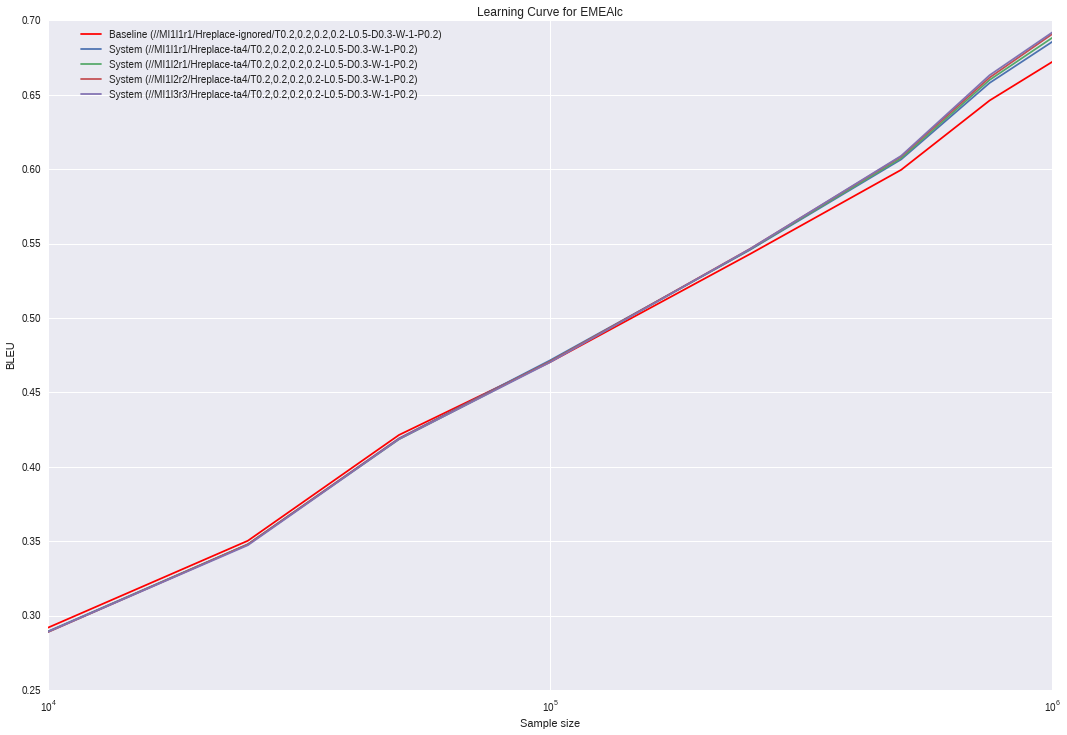
\includegraphics[width=120.00mm]{emealcbleu.png}
\caption{Learning curve on EMEA, English to Spanish, measuring BLEU score, logarithmic scale}
\label{fig:emealc}
\end{figure}


\begin{figure}
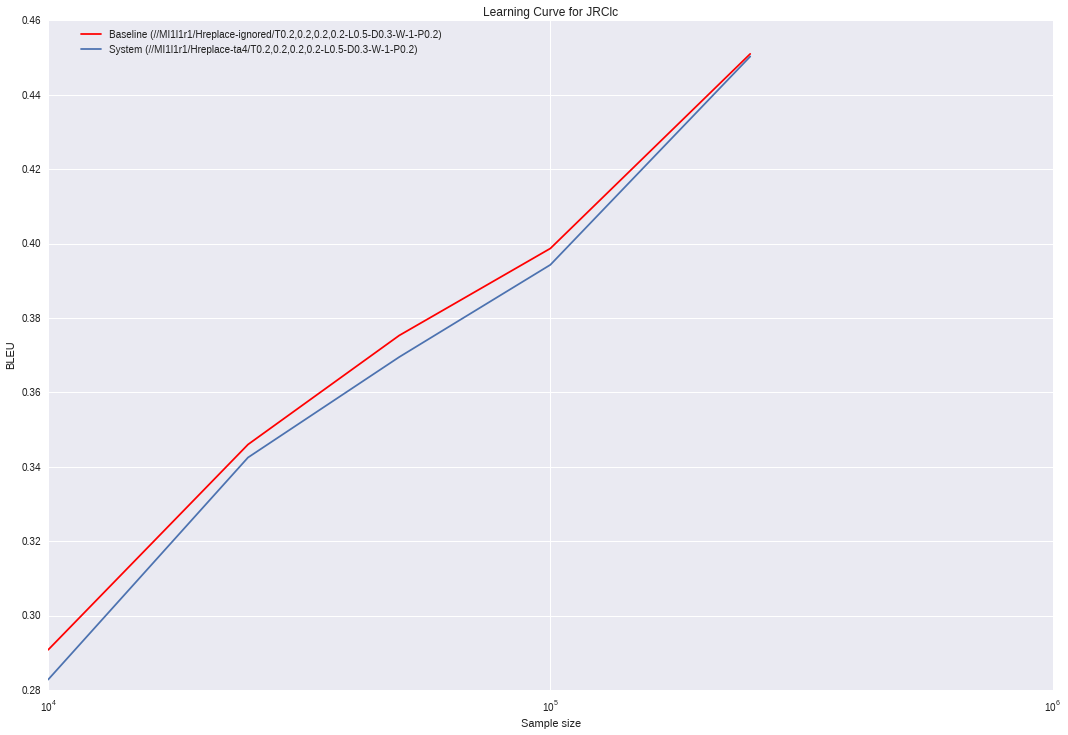
\includegraphics[width=120.00mm]{jrclcbleu.png}
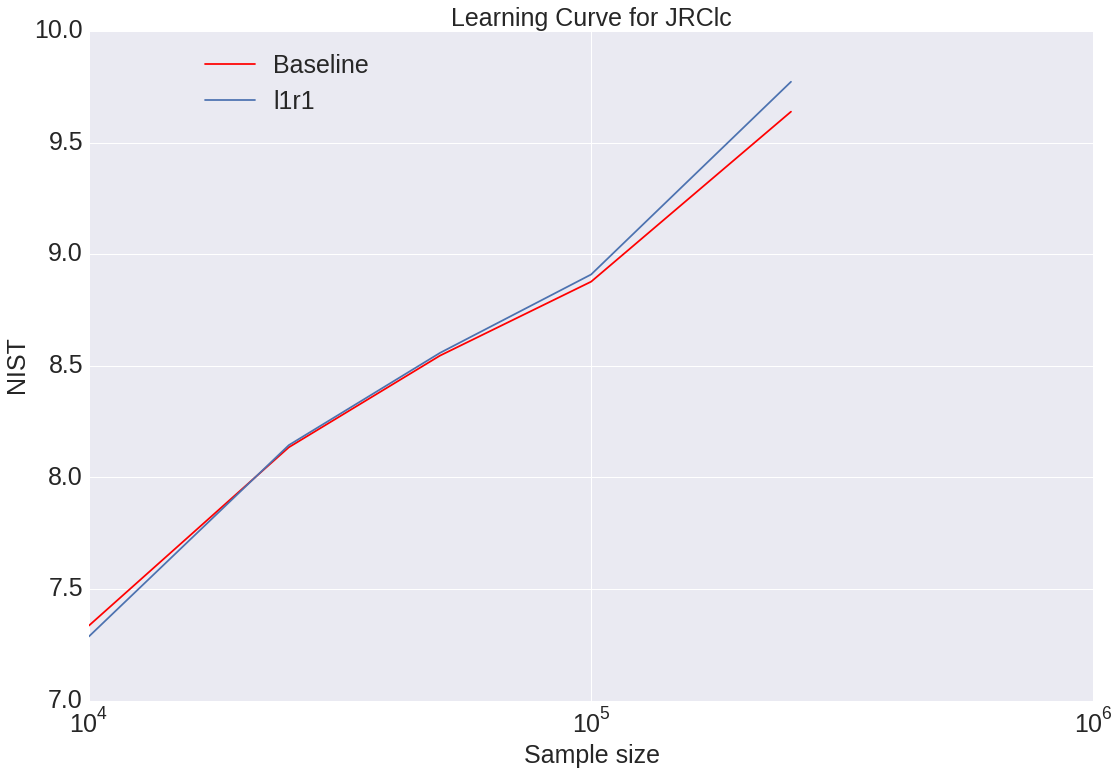
\includegraphics[width=120.00mm]{jrclcnist.png}
\caption{Learning curve on JRC Acquis, English to Spanish, measuring BLEU score (top) and NIST (bottom), logarithmic scale}
\label{fig:jrclc}
\end{figure}


In the EMEA learning curve in Table~\ref{fig:emealc}, we included an analysis
of different context sizes.  An enlargement of the context size seems to be
beneficial for this data set each step along the way, but these results have
already been shown not to generalise easily, nor is this trend likely to
continue if ever more context were to be added.

The positive results on the EMEA and JRC data needs to be contrasted to the
earlier negative results. Can we identify why these corpora, with these
language pairs, perform well?

We can observe that the nature of these two corpora consists of highly
formulaic language, medical language in the case of EMEA, and judicial language
in the case of JRC-Acquis.  This is implies the language is generally more
rigidly structured, predictable, and therefore easier to translate than corpora
from more diverse domains. The fact that the scores for these corpora are
higher than those for the corpora we've seen before illustrates this point.

As hypothesised earlier, it may be possible that a certain quality of
translation is needed before the source-side context information is able to
make an impact. The learning curve experiments suggest this, but it is at odds
with the positive results on the Chinese-English IWSLT 2006 data
(Table~\ref{tab:iwslt2006zhen}), which shows lower scores and is trained on a very
small training set. We dive further into this hypothesis with a series of
experiments on a Dutch-Frisian corpus. The high similarity between these two
Germanic languages of The Netherlands makes translation easier, and has been
shown to achieve high scores \citep{OERSETTER}. Table~\ref{tab:fa2} shows our
findings. Although high scores were obtained as expected, we were completely
unable to exceed the non-context-informed baseline. 

\begin{table}
\begin{tabular}{|l|ccccc|}
\hline
\textbf{System} & \textsc{BLEU}  & \textsc{METEOR}  & \textsc{NIST}  & \textsc{WER}  & \textsc{PER}  \\ 
\hline
\multicolumn{6}{|c|}{Fryske Akademy -- Frisian$\rightarrow$Dutch} \\
\hline 
Baseline (replace/M/opt) & \textbf{0.5572} & \textbf{0.7084} & \textbf{10.3162} & \textbf{29.86} & \textbf{24.73} \\ 
l1r1 (monolithic/replace/opt/tribl2) & 0.5544 & 0.7066 & 10.2967 & 30.08 & 24.91 \\ 
l1r1 (experts/replace/opt/ib1) & 0.5566 & 0.7077 & 10.3136 & 29.96 & 24.81 \\ 
\hline
\multicolumn{6}{|c|}{Fryske Akademy -- Dutch$\rightarrow$Frisian} \\
\hline
Baseline (replace/M/opt) & \textbf{0.5222} & \textbf{0.6911} & \textbf{9.9762} & \textbf{32.68} & \textbf{27.28} \\ 
l1r1 (monolithic/replace/opt/tribl2) & 0.5154 & 0.6857 & 9.9122 & 33.09 & 27.71 \\ 
l1r1 (experts/replace/opt/ib1) & 0.5164 & 0.6869 & 9.9258 & 33.0 & 27.59 \\ 
l2r1 (monolithic/replace/opt/tribl2) & 0.5145 & 0.6849 & 9.8992 & 33.16 & 27.78 \\ 
l2r1 (experts/replace/opt/ib1) & 0.5155 & 0.6864 & 9.9110 & 33.05 & 27.65 \\ 
l2r2 (monolithic/replace/opt/tribl2) & 0.5130 & 0.6841 & 9.8885 & 33.28 & 27.84 \\ 
l2r2 (experts/replace/opt/ib1) & 0.5157 & 0.6866 & 9.9159 & 33.05 & 27.61 \\ 
l3r3 (monolithic/replace/opt/tribl2) & 0.5114 & 0.6832 & 9.8656 & 33.41 & 27.97 \\ 
l3r3 (experts/replace/opt/ib1) & 0.5134 & 0.6852 & 9.8908 & 33.21 & 27.79 \\ 
\hline
\end{tabular}
\caption{Results on the Frisian-Dutch parallel corpus}
\label{tab:fa2}
\end{table}


We further address the issue of domain in a cross-domain experiment, to assess
whether introducing a differentiation between domains has a positive impact
when source-side context information is included. We did this for Dutch to
English, trained on 250,000 instances of the Europarl parallel corpus, and
tested on the IWSLT 2012 TED data. We find the context-informed
system\footnote{l1r1 (monolithic/replace/uni/tribl2)} scoring the
same\footnote{BLEU 0.2137, METEOR 0.4798, NIST 6.2172, WER 57.99, PER 46.01} as
the baseline, and thus not providing any added value. Unsurprisingly, scores
are considerably lower than when tested on the same domain (c.f
Table~\ref{tab:europarl250k}).

The below-baseline results for Dutch-English on two corpora (Europarl and IWSLT
2012 TED) may suggest that the efficacy of source-side context modelling
depends strongly on the language pair. A possible hypothesis here is that
source-side context modelling stands to gain most when translation from
morphologically simpler languages to morphologically richer languages, as the
source-side context information may help in determining the proper
morphological form. 

We test this hypothesis by conducting two experiments. All of the positive
results hitherto have been on language pairs in which the target language was
morphologically richer.  In the first experiment we therefore take such a
language pair, the English to Spanish language pair, and use it for a corpus
that has performed poorly: the 250,000 sentence subset of Europarl.  If the
results are better with English to Spanish than with Dutch to English then our
hypothesis would be strengthens our hypothesis. When we look at the results of
this experiment in Table~\ref{tab:europarl250k}, however, we immediately see
that this is not the case; all results are below baseline. A possible
explanation may be that more training data is needed, as suggested by the
earlier learning curves, but this too was an hypothesis we could not confirm on
another data set.

\begin{table}
\begin{tabular}{|l|ccccc|}
\textbf{System} & \textsc{BLEU}  & \textsc{METEOR}  & \textsc{NIST}  & \textsc{WER}  & \textsc{PER}  \\ 
\hline
\multicolumn{6}{c}{Europarl 250k - English $\rightarrow$ Spanish} \\
\hline 
Baseline (replace/M/opt) & \textbf{0.3424} & \textbf{0.5718} & 7.9896 & 53.64 & 39.2 \\ 
l1r1 (monolithic/replace/opt/tribl2) & 0.336 & 0.5666 & 7.9981 & 53.6 & 39.27 \\ 
l1r1 (experts/replace/opt/ib1) & 0.338 & 0.5677 & \textbf{8.0165} & \textbf{53.48} & \textbf{39.19} \\ 
l2r1 (monolithic/replace/opt/tribl2) & 0.3344 & 0.5651 & 7.993 & 53.63 & 39.3 \\ 
l2r1 (experts/replace/opt/ib1) & 0.3357 & 0.5664 & 8.0086 & 53.51 & 39.23 \\ 
l2r2 (monolithic/replace/opt/tribl2) & 0.3325 & 0.5639 & 7.9843 & 53.6 & 39.36 \\ 
l2r2 (experts/replace/opt/ib1) & 0.3345 & 0.5649 & 8.0 & 53.55 & 39.32 \\ 
l3r3 (monolithic/replace/opt/tribl2) & 0.329 & 0.5611 & 7.9518 & 53.74 & 39.61 \\ 
l3r3 (experts/replace/opt/ib1) & 0.3298 & 0.562 & 7.9593 & 53.79 & 39.57 \\ 
\hline
\end{tabular}
\caption{Negative results on Europarl 250k - English to Spanish}
\label{tab:europarl250k}
\end{table}

The second attempt to test this hypothesis focusses on English to Russian, a
very morphologically rich language with three genders and six cases. Under our
hypothesis, we would expect positive results here.  Table~\ref{tab:yandex1M}
shows the results of this experiment, but here we also find below-baseline
results that do not support our hypothesis.

\begin{table}
\begin{tabular}{|l|ccccc|}
\textbf{System} & \textsc{BLEU}  & \textsc{METEOR}  & \textsc{NIST}  & \textsc{WER}  & \textsc{PER}  \\ 
\hline
\multicolumn{6}{c}{yandex1M - English $\rightarrow$ Russian} \\
\hline
Baseline (replace/M/opt) & \textbf{0.1179} & \textbf{0.5579} & \textbf{5.2793} & 74.65 & 63.9 \\ 
l1r1 (monolithic/replace/opt/tribl2) & 0.1166 & 0.5568 & 5.2558 & \textbf{74.45} & \textbf{63.72} \\ 
\hline
\end{tabular}
\caption{Negative results on Yandex1M - English to Russian}
\label{tab:yandex1M}
\end{table}


\subsection{Results: classifier type and classifier parameter optimisation}
\label{sec:typeopt}

We have introduced two types of classifier, integrated in an Statistical
Machine Translation framework by means of the ``bypass'' method described in
Section~\ref{sec:smtintegration}. The monolithic classifier, modelling all phrase-pairs
in a single classifier, is used also by \cite{Stroppa+07} and
\cite{Rejwanul+11}, whereas the classifiers experts, one classifier per
source-phrase, is a new addition that more closely resembles how such
classifiers are employed in Word Sense Disambiguation.

Classifier experts were built using the IB1 algorithm, whereas we choose for
TRIBL2 for the monolithic classifier. This was done because the monolithic
classifier is a lot bigger by definition, and therefore the high performance of
the algorithm IGTree becomes imperative, a pure IB1 approach would be too slow
and TRIBL2 seeks to combine the best of both worlds.

Table~\ref{tab:expertcount} lists the number of classifier experts that were
built for some of the data sets. The actual number of source phrases is always
much higher, as classifiers are only built when there is ambiguity regarding
the translation. To see how these classifiers are typically distributed, based
on the number of instances and classes, we zoom in on the IWSLT 2012 data for
Dutch to English, and plot a histogram in Figure~\ref{fig:histogram}. As is
ubiquitous in natural language processing, a zipf curve can be discerned from
this figure, with the vast majority of classifier experts being very small and
having few translations options, i.e classes, and an immediate sharp drop in
frequency as the number of instances or classes increases.

\begin{table}
\begin{tabular}{|lll|l|}
\hline
\textbf{Corpus} & \textbf{Sentence pairs} & \textbf{Languages} & \textbf{Classifier Experts} \\
\hline
Europarl & 250,000 & English-Spanish & 828,326 \\
JRC & 250,000 & English-Spanish & 635,547 \\
IWSLT 2012 TED & 127,806 & Dutch-English & 193,811 \\
IWSLT 2006 & 40,274 & Chinese-English & 22,212 \\
Fryske Akademy & 137,937 & Dutch-Frisian & 276,819 \\
Fryske Akademy & 137,937 & Frisian-Dutch & 213,573 \\
\hline
\end{tabular}
\caption{Number of classifier experts generated per data set}
\label{tab:expertcount}
\end{table}


\begin{figure}
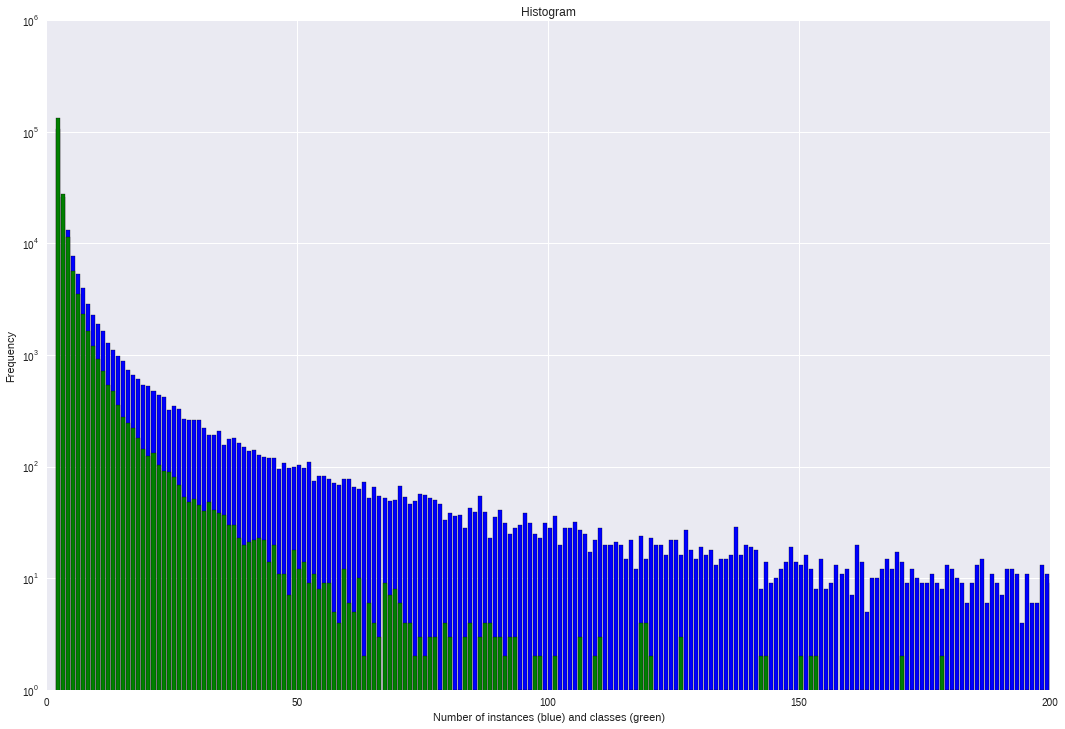
\includegraphics[width=80.00mm]{classifierhistogram.png}
\caption{Histogram showing the distribution of the number of instances (blue) and number of classes (green) in the classifier experts for IWSLT 2012 TED, Dutch to English (logarithmic)}
\label{fig:histogram}
\end{figure}

Most of the tables in Section~\ref{sec:results1} list results for both classifier
types.  We find the classifier experts outperforming the monolithic classifier
for Chinese-English (Table~\ref{tab:iwslt2006zhen} (for all context sizes except
\texttt{l3r3}), for  IWSTL 2012 TED Dutch-English (Table~\ref{tab:iwslt2012},
mostly below baseline), Europarl250k Dutch-English
(Table~\ref{tab:europarl250k}, mostly below baseline), and Frisian-Dutch
(Table~\ref{tab:fa2}, all below baseline)).

These results suggest that the classifier experts perform better than the
monolithic classifier. When looking at the two 250,000 instance samples of
JRC-Acquis (Table~\ref{tab:jrc250k}), we see a conflicting image. One sample
confirms our hypothesis that the classifier experts are better, whereas in the
other the monolithic classifier has the upper-hand. Moreover, when we look at
the EMEA data (Table~\ref{tab:emea}), where we had the most significant gains
above baseline, we find the monolithic system strongest. 

Despite the results not being unanimous, the case for the classifier experts is
strong and can be motivated by the fact that feature weights are computed on a per-
source-phrase basis, rather than on the aggregation of all. It can be considered as a
kind of optimisation step. The disadvantage is that such systems may therefore
be more prone to overfitting on one hand, which might well be the case in the
EMEA experiment, as well as sparsity problems for smaller classifier experts on
the other hand.

\todo{TODO: parameter optimisation experiment (still to run and process)}


\subsection{Results: Weighting methods and score analysis}
\label{sec:weighting}

Two weighting methods have been implemented, the \emph{append} method, adding
$p(t|s,C)$ as an extra score to the score vector, and the \emph{replace}
method, which replaces the existing $p(t|s)$ score with $p(t|s,C)$. Most
experiments have been conducted with the \emph{replace} method, as it is the
simplest one. For EMEA (Table~\ref{tab:emea}) and JRC-Acquis
(Table~\ref{tab:jrc250k}), the \emph{append} method was tested as well.

Comparing the two weighting methods, however, is far from trivial. When a
discrepancy is found between a run with the replace method (4 scores) and the
run with the append method (5 scores), we can not simply ascribe such a
difference to the extra score, but must into account that the very act of
adding a score shifts the weights for the score vector, even if uniformly
distributed. Any shift may likely affect the outcome. This
motivation is also the reason we included a separate baseline for the append
method in the tables in which we reported it. Moreover, it explains why we can
not just apply the results of the parameter optimisation of the replace method
to the append method.

Tables~\ref{tab:emea} (EMEA) and \ref{tab:jrc250k} (JRC) have been run without
parameter optimisation. Even without context information, the baselines for the
append method score better than those for the replace method. Effectively, the
append method's baseline is simply a version with a double feature and
functionally equivalent to just assigning double weight to the feature.

A comparison is complicated by the fact that the $p(t|s,C)$ score is often simply
equal to the $p(t|s)$ score, by definition so for any source phrases for which no
classifier was needed, due to not being ambiguous in translation or context. 

We can therefore not draw any satisfactory conclusions on the merit of the
\emph{append} method versus the \emph{replace} method, given the experiments we
conducted. We can, however, use the two different scoring methods to provide
insight into the classifier results. How often does the classifier assign a
$P(t|s,C)$ that significantly differs from $P(t|s)$? And how often are they
completely identical?

Such an analysis has been conducted on the test data of the JRC-Acquis
corpus,from English to Spanish. This is shown in
Figure~\ref{fig:scoredifference}. 

For each occurrence of each source phrase in the test-data, we gathered all
possible translations and computed $\frac{P(t|s,C)}{P(t|s)}$. This ratio
expresses the difference between the context-informed translation probability
and the non-context informed one.

A value of one indicates there is no difference whatsoever, this includes all
source phrases where either translation or context are unambiguous. A spike can
be observed at this point, this spike covers $9\%$ of phrase-pairs. The right
hand side of the graph ($>1$), is of most interest, it covers the phrase-pairs
for which the classifier increased the probability, we compute that $75\%$ of
the phrase-pairs is in this region, which is reflected by the increased
noise in the graph. 

%A downward trend can be observed in the graph, downward adjustments are more
%prevalent as it it is a logical consequence of increasing probability to one
%translation over the others in a distribution.

\begin{figure}
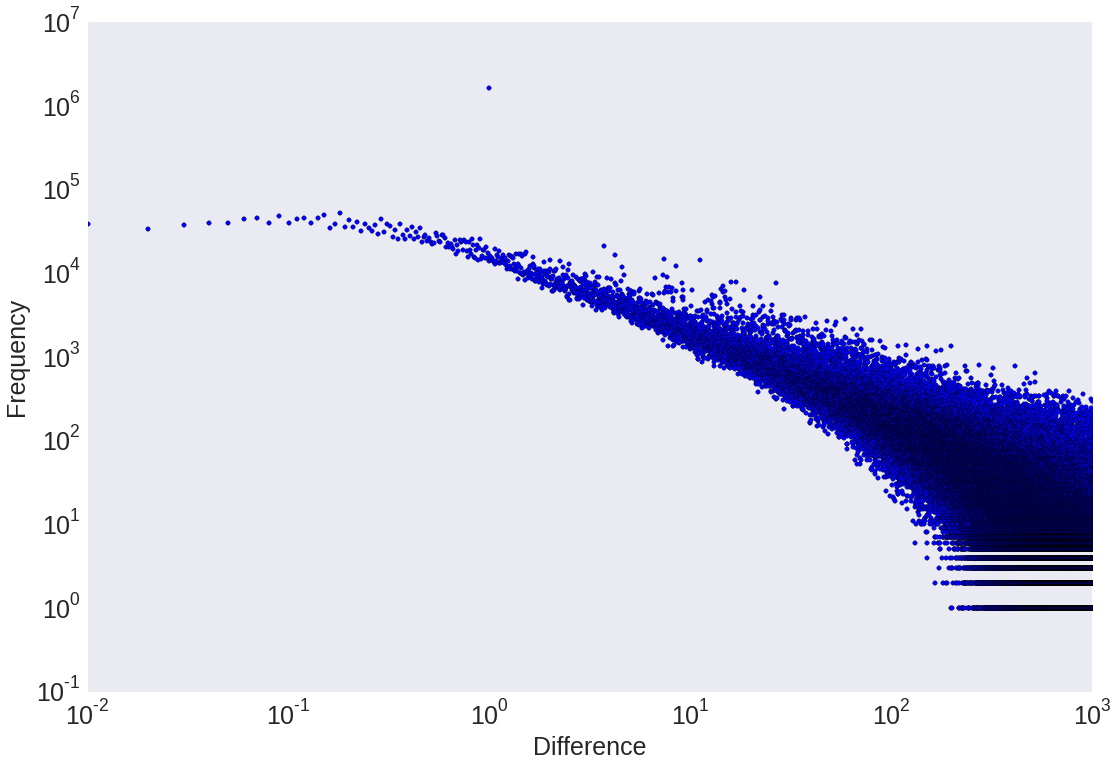
\includegraphics[width=80.00mm]{scoredifference.png}
\caption{Histogram in logarithmic scale showing the ratio $\frac{P(t|s,C)}{P(t|s)}$ for JRC250k English to Spanish test set, illustrating the difference between the classifier score and the original SMT score.}
\label{fig:scoredifference}
\end{figure}

\todo{TODO: Is this interpretation and visualisation clear enough?}

\subsection{Results: Qualitative Analysis}

In this section we will take a look at the translations themselves and see if
we can discern patterns that can tell us what the effect of source-side context
information is and when it pays off.

We zoom in on the corpus that performed best, the EMEA corpus -- English to
Spanish, one million sentence pairs. We compare the context-informed
\texttt{l1r1} system with the non-context informed baseline to assess the
impact of the context information. Out of $5000$ sentences in the test set,
$3863$ ($77\%$) are translated identically. This high number again shows that
it is difficult to make a difference. Nevertheless, $22\%$ differs and results
in a net gain in translation performance, as seen in Table~\ref{tab:EMEA}.

The next few examples will show some comparisons in which the context-informed
improves over the baseline. 

Example~\ref{ex:QAsynonym} shows three examples of the selection of a better
translation given the context, matching with the reference translation, even
though the baseline translation could be considered correct as well. This is
the most common type of difference. Example~\ref{ex:QAdrop} shows the dropping
of a word.


\begin{exmp}
\footnotesize
\label{ex:QAsynonym}
\textbf{Baseline:} El cambio continuo del lugar de inyección dentro de \underline{un área} determinada puede ayudar a \\
\textbf{l1r1:} El cambio continuo del lugar de inyección dentro de \underline{una región} determinada puede ayudar a \\
\textbf{Reference:} La contínua rotación de los puntos de inyección dentro de \underline{una región} determinada puede ayudar a reducir o prevenir estas reacciones \\
\noindent\makebox[\linewidth]{\rule{\linewidth}{0.4pt}}
\textbf{Baseline:} Baraclude reduce la cantidad de virus en su \underline{cuerpo} y mejora el estado del hígado . \\
\textbf{l1r1:} Baraclude reduce la cantidad de virus en su \underline{organismo} y mejora el estado del hígado  \\
\textbf{Reference:} Baraclude reduce la cantidad de virus en su \underline{organismo} y mejora el estado del hígado .
\\ 
\noindent\makebox[\linewidth]{\rule{\linewidth}{0.4pt}}
\textbf{Baseline:} Como consecuencia , el fenilbutirato de sodio , reduce \underline{los niveles plasmáticos} de amonio y glutamina en pacientes con trastornos del ciclo de la urea . \\
\textbf{l1r1:} Como consecuencia , el fenilbutirato de sodio reduce \underline{las concentraciones plasmáticas elevadas} de amonio y glutamina en pacientes con trastornos del ciclo de la urea .  \\
\textbf{Reference:} Como consecuencia , el fenilbutirato de sodio reduce \underline{las concentraciones plasmáticas elevadas} de amoníaco y glutamina en pacientes con trastornos del ciclo de la urea .
\end{exmp}

\begin{exmp}
\footnotesize
\label{ex:QAdrop}
\textbf{Baseline:} \underline{Los estudios} en animales , no pueden excluir el desarrollo potencial de toxicidad ( ver sección 5.3 ) . \\
\textbf{l1r1:} \underline{Estudios} en animales , no pueden excluir el desarrollo potencial de toxicidad ( ver sección 5.3 ) . \\
\textbf{Reference:} \underline{Estudios} en animales , no pueden excluir el desarrollo potencial de toxicidad ( ver sección 5.3 ) .
\end{exmp}

\begin{exmp}
\footnotesize
\label{ex:QAgrammar}
\textbf{Baseline:} Las reacciones adversas \underline{consideradas relacionadas} con el uso de Agenerase son síntomas gastrointestinales , erupción y parestesia oral / peri-oral . \\
\textbf{l1r1:}  Las reacciones adversas \underline{que se consideran relacionadas} con el uso de Agenerase son síntomas gastrointestinales , erupción y parestesia oral / \\
\textbf{Reference:} Las reacciones adversas \underline{que se consideran relacionadas} con el uso de Agenerase son síntomas gastrointestinales , erupción y parestesia oral / perioral . \\ \\
\end{exmp}

In addition to the positive examples, there are also neutral and negative examples. In example~\ref{ex:QAneutral}, all translations can be considered correct and conveying the same message with different nuances, as a difference construction is chosen. Example~\ref{ex:QAnegative} shows the inverse situation of example~\ref{ex:QAsynonym}, a different synonym was chosen but it does not match with the reference translation. This too is a common pattern in the data. This raises the question whether the impact of context-information would not be lower if the test set would have contained multiple reference translations. Such data unfortunately is hard to come by and was not available in this study.

\begin{exmp}
\footnotesize
\label{ex:QAneutral}
\textbf{Baseline:} Asegúrese de que el polvo \underline{esté completamente disuelto} . \\
\textbf{l1r1:} Asegúrese de que el polvo \underline{se disuelva completamente} .  \\
\textbf{Reference:} Asegúrese de que el polvo \underline{se ha disuelto completamente} .
\end{exmp}

\begin{exmp}
\footnotesize
\label{ex:QAnegative}
\textbf{Baseline:} Los pacientes \underline{se asignaron aleatoriamente} a recibir 500 $\mu$ g de Aranesp una vez cada tres semanas o 2,25 $\mu$ g / kg una vez a la semana . \\
\textbf{l1r1:} Los pacientes \underline{fueron aleatorizados} a recibir 500 $\mu$ g de Aranesp una vez cada tres semanas o 2,25 $\mu$ g / kg una vez a la semana . \\
\textbf{Reference:} Los pacientes \underline{se asignaron aleatoriamente} a recibir 500 $\mu$ g de Aranesp una vez cada tres semanas o 2,25 $\mu$ g / kg una vez a la semana .
\end{exmp}


\section{Conclusion \& Discussion} 

We have conducted numerous experiments to assess whether surface-form
source-side context information, i.e. without the use of any explicit
linguistic features that require supervised parsers or taggers, can improve
translation quality. Memory-based classifiers were used, and integrated in an
SMT framework, following techniques commonly employed in WSD. The results of
the experiments were mixed and there was a high degree of variability between
different corpora and language pairs. Positive results were attained on only
EMEA and JRC-Acquis, highly formulaic corpora. 

We replicated part of the work of \cite{Stroppa+07} and \cite{Rejwanul+11}, and
found that results are fairly marginal. Inclusion of surface-form
source-side context information is clearly not the most obvious road for the
improvement of MT quality. It is likely that improvement can be more easily
achieved through simple improvement of the target-side language model.

We hypothesised that source-side context information may contribute more when
translating to a morpholigically more complex language, but were unable to
prove this hypothesis. 

In this discussion, we would like to focus on why the results of our study over-all do not make a good impression above baseline.  There is a theoretical foundation for this
if we look at the interplay between the SMT decoder and the classifiers. For a
source phrase $s$ with context $C$ and mapping to translation $t$ to be a
strong fragment in the classifier, it has to have been observed multiple times
in the training data. If this is so, then there is often a source fragment $s'$
in the phrase-translation table that is the conjunction of $s$ and $C$, and
which maps to a $t'$ of which $t$ is at least a substring. It is thus likely that the
context information we try to explicitly model, is often already implicitly
available to the decoder. This is provided that the classifier and
phrase-translation table are trained on the same parallel corpus, as we
consistently did.



\todo{TODO: finish}


\bibliographystyle{spbasic}
\bibliography{sourcecontextinsmt}




\end{document}

\chapter{Summary \& Conclusion}
\label{chap:conclusion}

In this dissertation, we posited the main hypothesis that inclusion of source-side context information, without
linguistically informed features, benefits translation quality. We have assessed this question from various different
angles. We set out to answer the following inter-related questions and have indeed largely already done so in
Section~\ref{sec:conclusion} of Chapter~\ref{chap:sourcecontextinsmt}:

\begin{enumerate}
\item To what extent can we improve translation by considering source-side
    context information?
\item What context features prove most effective?
\item To what extent are linguistically uninformed features effective?
\item How can source-side classifiers be used in translation tasks?
\end{enumerate}

Chapter~\ref{chap:clwsd} demonstrated an application in cross-lingual word sense
disambiguation, where word expert classifiers succesfully tackled the problem
of translating a word in context. Our system emerged as the winning system in
the SemEval 2010 Cross Lingual Word Sense Disambiguation task, and achieved
either winning or high scores in the same task in 2012. This second time
around, we placed focus on hyperparameter optimisation of the classifier
parameters and automatic feature selection per classifier expert, which
supersedes the voting approach we used the first time. Automatic feature
selection indeed leads to a modest improvement, whereas classifier parameter
optimisation does not.

At this stage, we experimented with some basic linguistically informed
features as well, i.e. part-of-speech tags and lemmas. Lemmas proved to be
beneficial indeed, whereas part-of-speech tags failed to make a positive
impact. Nevertheless, our study's explicit focus is to assess the efficacy of
the surface features in their pure form, i.e. not enriched with any linguistic
information. We employed multiple classifiers or word experts in which the
feature vector consists of a simple local context window. In the cross-lingual
WSD task our linguistically-uninformed classifiers easily surpass the
non-context-informed baselines. In other words, for this task, we find evidence that
corroborates our main hypothesis and gives positive support to our first and third question.

We extensively experimented with global context features at this stage, as
opposed to local context features found in the immediate neighbourhood of the
phrase to be translated. We found a discrepancy in results between the SemEval
2010 and 2012 runs. Subsequent attempts in later chapters support the SemEval
2012 findings, in which global context features do not lead to an improvement
in translation quality.

The initial successes with translation aided by source-side context information
led us to propose this technique for a novel application in computer-aided translation
assistance. In this task, we translate L1 fragments in an L2 context.
In Chapter~\ref{chap:colibritapilot} we tested the feasibility of this idea and
found our context-sensitive classifiers improve both upon a non-context informed
baseline, as well a baseline enriched with a language model. We then
proposed our task for SemEval 2014 in Chapter~\ref{chap:semeval2014task5}, and attracted
participation by six participants, some of whom achieve high results. It
becomes apparent, specifically, that phrase-based statistical machine translation is able to
achieve better results than pure classifier-based approaches, despite the
localised and cross-lingual nature of the task.

We confirm this in Chapter~\ref{chap:colibritafinal}, where we conducted an
extensive comparison of the pure classifier-based and SMT-based solutions to
our L2 Translation Assistance task. We then proceed to integrate classifiers in
the SMT-based solution, in an attempt to gain the best of both worlds. However,
we find that this does not lead to improved translation quality. Nevertheless,
our hypothesis that translation can be improved by considering source-side
context information is still upheld here.

In Chapter~\ref{chap:sourcecontextinsmt} we moved away from the translation of
mere localised fragments in a context, and experimented with full Statistical
Machine Translation, i.e. translation of whole sentences. We incorporated
source-side context information using classifiers in the SMT decoder, using a
bypass method. We tested various forms of integration, but found that we could
only really improve upon the baseline for one corpus (IWSLT 2006, Chinese to
English). All other results turned out on or below baseline, or failed to pass
rigourous significance tests. Our main hypothesis therefore does not hold for
full statistical machine translation. We ask ourselves why this is the case and
suggest that that the information we attempt to explicitly model in the
translation model, is already implicitly and satisfactorily covered by both the
target-side language model as well as the translation model. Integration of
linguistically-uninformed classifiers in statistical machine translation
therefore has no added value.

Our efforts only prove fruitful when used standalone or for localised problems,
whereas statistical machine translation proves to be a superior technique,
leading to higher translation quality, for those translation tasks that it can
tackle.

When it comes to classifiers and their integration in SMT, future research could continue in the direction that
past studies such as \cite{Rejwanul+11} have already proceeded; that of incorporating linguistic
features. The technical foundation for such studies is well prepared in this one: The integration and score weighting methods from Chapters~\ref{chap:colibritafinal} and especially
\ref{chap:sourcecontextinsmt} lay a foundation upon which expansions with specific linguistic features would make this a
feasible option. We do not think, however, that this is a promising line of continued investigation as the
novelty of such further studies would be limited, depending on the type of linguistic features
investigated and the way they are incorporated. Moreover, results from participants of our SemEval task, show
that intuitively promising linguistically-informed features, such as dependency features, do not always lead to the
expected improvement \citep{UNAL,IUCL}.

We especially have to concede that the state-of-the-art in Machine Translation has changed considerably during and after
the years this research has taken place; techniques such as Neural Machine Translation have appeared on stage and often
prove superior to the SMT paradigm we employed. What the possibilities of source-side context in Neural Machine
Translation are, is already an active subject of research \citep{Jean+17,Wang+17,Bawden+17,Maruf+17}. These studies
do mostly focus on wider discourse context than we did.

The academic merit of our study is primarily in deepening and closing a line of investigation; that of modelling
source-side context information, mostly through memory-based classifiers, and integration thereof in Statistical Machine
Translation. We have dived to considerable depth, beyond that of prior studies, to
squeeze whatever we could out of these techniques at our disposition, and to study their interplay in various settings.
At the same time, we subjected our experiments to high standards by testing on a wide variety of corpora, language pairs and incorporating necessary statistical significance tests.

Aside from the answers to the research questions provided by this dissertation, other notable contributions this research
project delivers are 1) the Colibri Core software that was developed and described in Chapter~\ref{chap:coco},
application of which goes well beyond what it was used for in this research; and 2) the cross-lingual translation
assistance task we proposed in Chapter~\ref{chap:semeval2014task5} and solutions to which were extensively studied.





\bibliographystyle{apalike}
\bibliography{thesis}

\chapter*{Summary}
\addcontentsline{toc}{chapter}{Summary}
\markboth{Summary}{Summary}

\emph{Context as Linguistic Bridges} is a study that focusses on the role of
context information in machine translation, i.e. automated translation by computers.  The
underlying intuition is that the context in which a word or phrase appears is
an important cue for the translation of that word or phrase; it helps in
resolving ambiguity.

Consider, for instance, the English word \emph{``bank''}, which can refer to a
financial institution or the bank of a river. In sentences such as \emph{``I
put my money on the bank''} and \emph{``The ship got stuck on the bank''}, the
context helps to disambiguate the word. Automatically identifying what the corredct sense of a word is, is known as Word Sense
Disambiguation (WSD). In this research we develop techniques to do this
in and attempt to apply these same techniques in a Machine
Translation context. After all, if we were to translate these two distinct
word senses to another language, we would likely obtain different words. For
Dutch we would get \emph{``bank''} and \emph{``oever''}, respectively.

We look into two particular solutions to solve two different problems and then
try to combine these into one: \emph{Memory-based Classification} proves
successful in Word Sense Disambiguation tasks, and \emph{Phrase-based
Statistical Machine Translation} used to be the state-of-the-art in machine
translation when this research began (but it has been superseded since by deep
learning). We combine these two techniques and attempt to answer the following main
question:

\begin{quote}
\emph{To what extent can we improve translation by considering source-side context information?}
\end{quote}

In this sense, ``source-side context'' refers to the fact that we use
information from the input in the source language, which is to be translated
into the target language.

We also add a twist to this research as we investigate a special type of
translation using source-side context; the translation of a word or phrase in a
cross-lingual context; a phenomenon also known as code-switching. Consider a
frenchman attempting to speak English (L2), but not finding quite the right
words for everything so reverting back to his native language (L1) for that
fragment: ``I go ...eh.... \emph{rentre à la maison}... because I am tired.''
. We try to automatically translate this L1 fragment in an L2 context to L2.

In our search for an answer to the main question, we can distinguish three subquestions that will be addressed:

\begin{itemize}
\item \emph{What context features prove most effective?} - What exactly in the source-side context provides the most valuable cue for a succesful disambiguation?
\item \emph{To what extent are linguistically uninformed features effective?} -  Our aim is to stay as close to the pure
    textual data as possible, not aided by further linguistic information such as part-of-speech tags or lemmas. We do
    conduct various experiments to see what difference such linguistic enrichment makes.
\item \emph{How can source-side classifiers be used in translation tasks?} - How exactly do we integrate classifiers inside a phrase-based statistical machine translation system? There are various possibilities and choices to make and we investigate and compare several.
\end{itemize}

We have to conclude that the integration of context-aware classifiers in a
phrase-based statistical machine translation system, does not lead to any
significant improvement, contrary to our initial hypothesis. This does not
discredit the idea that source-side context provides valuable cues for
translation or disambiguation, as we show in our WSD research.  It shows only
that modelling this source-side context information explicitly provides no
extra benefit over the already existing statistical machine translation model, and we infer
that the information is already available implicitly to a sufficient degree in the
existing statistical machine translation model.


\chapter*{Curriculum Vitae}
\addcontentsline{toc}{chapter}{Curriculum Vitae}
\markboth{Curriculum Vitae}{Curriculum Vitae}

Maarten van Gompel was born on the \nth{15} of December 1982, in Etten-Leur,
the Netherlands. After completing his secondary education (VWO) at the
Heerbeeck College in Best in 2002, he enrolled in the study of
Cognitive Artificial Intelligence (CKI) at Utrecht University,
seeking a bachelor study that would combine his
passion for both language as well as technology. He also
co-founded the UniLang Language Community, one of the first communities on the
internet for language enthusiasts and polyglots to unite and learn languages,
that thrived in the early 2000s before the advent of social media. He obtained
the degree of Bachelor of Science from Utrecht University in 2008 and then
switched to Tilburg University for his master degree in ``Human Aspects of
Information Technology'', looking for a stronger focus on Natural Language
Processing (NLP).  This resulted in the degree of Master of Arts in 2009.

He stayed in Tilburg at the Induction of Linguistic Knowledge (ILK) research
group, led by prof. dr. Antal van den Bosch, for the next two years where he was working on
the DutchSemCor project as a scientific programmer. Around this time, he also
got involved in the CLARIN project and started two software
initiatives, CLAM (a tool to quickly create webservices out of NLP tools) and
FoLiA (a Format for Linguistic Annotation), for which he in 2015 received the CLARIN Young Scientist Award. Both projects
still in active development to this day, a decade later, and have provided a foundation for a lot of his later work.

In 2011, Antal van den Bosch and Maarten van Gompel transferred to Radboud
University, Nijmegen, where the PhD research started. The research group that
formed over the years came to be known as the ``Lamas'', short for ``Language
Machines''.  Alongside his work on this PhD research, Maarten has been actively
working as a research software engineer. As an avid open-source and free
software proponent, he is involved in initiatives promoting good software
quality \& sustainability practices in the research community. He created and
maintains various software tools, including the Colibri Core software that
culminated from his PhD project.

Though the formal conclusion of the PhD research was delayed until 2020, the
actual research already reached its conclusion in 2016, and ever since he has
been working on software development for, amongst others, the CLARIAH and
Nederlab projects, as well as performing duties in Linux system administration.

%Obtained from http://www.siks.nl/siks_dissertations.ltx at 2020-01-08
\appendix*{SIKS Dissertation Series}

%\begin{longtable}{@{}l@{ }l@{\hspace{1em}}X}
\begin{longtabu}{@{}l@{ }l@{\hspace{1em}}X}
\toprule
2011	&	 01	&	 Botond Cseke (RUN), Variational Algorithms for Bayesian Inference in Latent Gaussian Models\\
	&	 02	&	 Nick Tinnemeier (UU), Organizing Agent Organizations. Syntax and Operational Semantics of an Organization-Oriented Programming Language\\
	&	 03	&	 Jan Martijn van der Werf (TUE), Compositional Design and Verification of Component-Based Information Systems\\
	&	 04	&	 Hado van Hasselt (UU), Insights in Reinforcement Learning; Formal analysis and empirical evaluation of temporal-difference\\
	&	 05	&	 Bas van der Raadt (VU), Enterprise Architecture Coming of Age - Increasing the Performance of an Emerging Discipline.\\
	&	 06	&	 Yiwen Wang (TUE), Semantically-Enhanced Recommendations in Cultural Heritage\\
	&	 07	&	 Yujia Cao (UT), Multimodal Information Presentation for High Load Human Computer Interaction\\
	&	 08	&	 Nieske Vergunst (UU), BDI-based Generation of Robust Task-Oriented Dialogues\\
	&	 09	&	 Tim de Jong (OU), Contextualised Mobile Media for Learning\\
	&	 10	&	 Bart Bogaert (UvT), Cloud Content Contention\\
	&	 11	&	 Dhaval Vyas (UT), Designing for Awareness: An Experience-focused HCI Perspective\\
	&	 12	&	 Carmen Bratosin (TUE), Grid Architecture for Distributed Process Mining\\
	&	 13	&	 Xiaoyu Mao (UvT), Airport under Control. Multiagent Scheduling for Airport Ground Handling\\
	&	 14	&	 Milan Lovric (EUR), Behavioral Finance and Agent-Based Artificial Markets\\
	&	 15	&	 Marijn Koolen (UvA), The Meaning of Structure: the Value of Link Evidence for Information Retrieval\\
	&	 16	&	 Maarten Schadd (UM), Selective Search in Games of Different Complexity\\
	&	 17	&	 Jiyin He (UVA), Exploring Topic Structure: Coherence, Diversity and Relatedness\\
	&	 18	&	 Mark Ponsen (UM), Strategic Decision-Making in complex games\\
	&	 19	&	 Ellen Rusman (OU), The Mind's Eye on Personal Profiles\\
	&	 20	&	 Qing Gu (VU), Guiding service-oriented software engineering - A view-based approach\\
	&	 21	&	 Linda Terlouw (TUD), Modularization and Specification of Service-Oriented Systems\\
	&	 22	&	 Junte Zhang (UVA), System Evaluation of Archival Description and Access\\
	&	 23	&	 Wouter Weerkamp (UVA), Finding People and their Utterances in Social Media\\
	&	 24	&	 Herwin van Welbergen (UT), Behavior Generation for Interpersonal Coordination with Virtual Humans On Specifying, Scheduling and Realizing Multimodal Virtual Human Behavior\\
	&	 25	&	 Syed Waqar ul Qounain Jaffry (VU), Analysis and Validation of Models for Trust Dynamics\\
	&	 26	&	 Matthijs Aart Pontier (VU), Virtual Agents for Human Communication - Emotion Regulation and Involvement-Distance Trade-Offs in Embodied Conversational Agents and Robots\\
	&	 27	&	 Aniel Bhulai (VU), Dynamic website optimization through autonomous management of design patterns\\
	&	 28	&	 Rianne Kaptein (UVA), Effective Focused Retrieval by Exploiting Query Context and Document Structure\\
	&	 29	&	 Faisal Kamiran (TUE), Discrimination-aware Classification\\
	&	 30	&	 Egon van den Broek (UT), Affective Signal Processing (ASP): Unraveling the mystery of emotions\\
	&	 31	&	 Ludo Waltman (EUR), Computational and Game-Theoretic Approaches for Modeling Bounded Rationality\\
	&	 32	&	 Nees-Jan van Eck (EUR), Methodological Advances in Bibliometric Mapping of Science\\
	&	 33	&	 Tom van der Weide (UU), Arguing to Motivate Decisions\\
	&	 34	&	 Paolo Turrini (UU), Strategic Reasoning in Interdependence: Logical and Game-theoretical Investigations\\
	&	 35	&	 Maaike Harbers (UU), Explaining Agent Behavior in Virtual Training\\
	&	 36	&	 Erik van der Spek (UU), Experiments in serious game design: a cognitive approach\\
	&	 37	&	 Adriana Burlutiu (RUN), Machine Learning for Pairwise Data, Applications for Preference Learning and Supervised Network Inference\\
	&	 38	&	 Nyree Lemmens (UM), Bee-inspired Distributed Optimization\\
	&	 39	&	 Joost Westra (UU), Organizing Adaptation using Agents in Serious Games\\
	&	 40	&	 Viktor Clerc (VU), Architectural Knowledge Management in Global Software Development\\
	&	 41	&	 Luan Ibraimi (UT), Cryptographically Enforced Distributed Data Access Control\\
	&	 42	&	 Michal Sindlar (UU), Explaining Behavior through Mental State Attribution\\
	&	 43	&	 Henk van der Schuur (UU), Process Improvement through Software Operation Knowledge\\
	&	 44	&	 Boris Reuderink (UT), Robust Brain-Computer Interfaces\\
	&	 45	&	 Herman Stehouwer (UvT), Statistical Language Models for Alternative Sequence Selection\\
	&	 46	&	 Beibei Hu (TUD), Towards Contextualized Information Delivery: A Rule-based Architecture for the Domain of Mobile Police Work\\
	&	 47	&	 Azizi Bin Ab Aziz (VU), Exploring Computational Models for Intelligent Support of Persons with Depression\\
	&	 48	&	 Mark Ter Maat (UT), Response Selection and Turn-taking for a Sensitive Artificial Listening Agent\\
	&	 49	&	 Andreea Niculescu (UT), Conversational interfaces for task-oriented spoken dialogues: design aspects influencing interaction quality\\

\midrule
2012&	 01	&	 Terry Kakeeto (UvT), Relationship Marketing for SMEs in Uganda\\
	&	 02	&	 Muhammad Umair (VU), Adaptivity, emotion, and Rationality in Human and Ambient Agent Models\\
	&	 03	&	 Adam Vanya (VU), Supporting Architecture Evolution by Mining Software Repositories\\
	&	 04	&	 Jurriaan Souer (UU), Development of Content Management System-based Web Applications\\
	&	 05	&	 Marijn Plomp (UU), Maturing Interorganisational Information Systems\\
	&	 06	&	 Wolfgang Reinhardt (OU), Awareness Support for Knowledge Workers in Research Networks\\
	&	 07	&	 Rianne van Lambalgen (VU), When the Going Gets Tough: Exploring Agent-based Models of Human Performance under Demanding Conditions\\
	&	 08	&	 Gerben de Vries (UVA), Kernel Methods for Vessel Trajectories\\
	&	 09	&	 Ricardo Neisse (UT), Trust and Privacy Management Support for Context-Aware Service Platforms\\
	&	 10	&	 David Smits (TUE), Towards a Generic Distributed Adaptive Hypermedia Environment\\
	&	 11	&	 J.C.B. Rantham Prabhakara (TUE), Process Mining in the Large: Preprocessing, Discovery, and Diagnostics\\
	&	 12	&	 Kees van der Sluijs (TUE), Model Driven Design and Data Integration in Semantic Web Information Systems\\
	&	 13	&	 Suleman Shahid (UvT), Fun and Face: Exploring non-verbal expressions of emotion during playful interactions\\
	&	 14	&	 Evgeny Knutov (TUE), Generic Adaptation Framework for Unifying Adaptive Web-based Systems\\
	&	 15	&	 Natalie van der Wal (VU), Social Agents. Agent-Based Modelling of Integrated Internal and Social Dynamics of Cognitive and Affective Processes.\\
	&	 16	&	 Fiemke Both (VU), Helping people by understanding them - Ambient Agents supporting task execution and depression treatment\\
	&	 17	&	 Amal Elgammal (UvT), Towards a Comprehensive Framework for Business Process Compliance\\
	&	 18	&	 Eltjo Poort (VU), 	Improving Solution Architecting Practices\\
	&	 19	&	 Helen Schonenberg (TUE), What's Next? Operational Support for Business Process Execution\\
	&	 20	&	 Ali Bahramisharif (RUN), Covert Visual Spatial Attention, a Robust Paradigm for Brain-Computer Interfacing\\
	&	 21	&	 Roberto Cornacchia (TUD), Querying Sparse Matrices for Information Retrieval\\
	&	 22	&	 Thijs Vis (UvT), Intelligence, politie en veiligheidsdienst: verenigbare grootheden?\\
	&	 23	&	 Christian Muehl (UT), Toward Affective Brain-Computer Interfaces: Exploring the Neurophysiology of Affect during Human Media Interaction\\
	&	 24	&	 Laurens van der Werff (UT), Evaluation of Noisy Transcripts for Spoken Document Retrieval\\
	&	 25	&	 Silja Eckartz (UT), Managing the Business Case Development in Inter-Organizational IT Projects: A Methodology and its Application\\
	&	 26	&	 Emile de Maat (UVA), Making Sense of Legal Text\\
	&	 27	&	 Hayrettin Gurkok (UT), Mind the Sheep! User Experience Evaluation \& Brain-Computer Interface Games\\
	&	 28	&	 Nancy Pascall (UvT), Engendering Technology Empowering Women\\
	&	 29	&	 Almer Tigelaar (UT), Peer-to-Peer Information Retrieval\\
	&	 30	&	 Alina Pommeranz (TUD), Designing Human-Centered Systems for Reflective Decision Making\\
	&	 31	&	 Emily Bagarukayo (RUN), A Learning by Construction Approach for Higher Order Cognitive Skills Improvement, Building Capacity and Infrastructure\\
	&	 32	&	 Wietske Visser (TUD), 	Qualitative multi-criteria preference representation and reasoning\\
	&	 33	&	 Rory Sie (OUN), Coalitions in Cooperation Networks (COCOON)\\
	&	 34	&	 Pavol Jancura (RUN), Evolutionary analysis in PPI networks and applications\\
	&	 35	&	 Evert Haasdijk (VU), Never Too Old To Learn -- On-line Evolution of Controllers in Swarm- and Modular Robotics\\
	&	 36	&	 Denis Ssebugwawo (RUN), Analysis and Evaluation of Collaborative Modeling Processes\\
	&	 37	&	 Agnes Nakakawa (RUN), A Collaboration Process for Enterprise Architecture Creation\\
	&	 38	&	 Selmar Smit (VU), Parameter Tuning and Scientific Testing in Evolutionary Algorithms\\
	&	 39	&	 Hassan Fatemi (UT), Risk-aware design of value and coordination networks\\
	&	 40	&	 Agus Gunawan (UvT), Information Access for SMEs in Indonesia\\
	&	 41	&	 Sebastian Kelle (OU), Game Design Patterns for Learning\\
	&	 42	&	 Dominique Verpoorten (OU), Reflection Amplifiers in self-regulated Learning\\
	&	 43	&	 Withdrawn \\
	&	 44	&	 Anna Tordai (VU), On Combining Alignment Techniques\\
	&	 45	&	 Benedikt Kratz (UvT), A Model and Language for Business-aware Transactions\\
	&	 46	&	 Simon Carter (UVA), Exploration and Exploitation of Multilingual Data for Statistical Machine Translation\\
	&	 47	&	 Manos Tsagkias (UVA), Mining Social Media: Tracking Content and Predicting Behavior\\
	&	 48	&	 Jorn Bakker (TUE), Handling Abrupt Changes in Evolving Time-series Data\\
	&	 49	&	 Michael Kaisers (UM), Learning against Learning - Evolutionary dynamics of reinforcement learning algorithms in strategic interactions\\
	&	 50	&	 Steven van Kervel (TUD), Ontologogy driven Enterprise Information Systems Engineering\\
	&	 51	&	 Jeroen de Jong (TUD), Heuristics in Dynamic Sceduling; a practical framework with a case study in elevator dispatching\\

\midrule
2013&    01	&    Viorel Milea (EUR), News Analytics for Financial Decision Support\\
	&	 02	&	 Erietta Liarou (CWI), MonetDB/DataCell: Leveraging the Column-store Database Technology for Efficient and Scalable Stream Processing\\
	&	 03	&	 Szymon Klarman (VU), Reasoning with Contexts in Description Logics\\
	&	 04	&	 Chetan Yadati (TUD), Coordinating autonomous planning and scheduling\\
	&	 05	&	 Dulce Pumareja (UT), Groupware Requirements Evolutions Patterns\\
	&	 06	&	 Romulo Goncalves (CWI), The Data Cyclotron: Juggling Data and Queries for a Data Warehouse Audience\\
	&	 07	&	 Giel van Lankveld (UvT), Quantifying Individual Player Differences\\
	&	 08	&	 Robbert-Jan Merk (VU), Making enemies: cognitive modeling for opponent agents in fighter pilot simulators\\
	&	 09	&	 Fabio Gori (RUN), Metagenomic Data Analysis: Computational Methods and Applications\\
	&	 10	&	 Jeewanie Jayasinghe Arachchige (UvT), A Unified Modeling Framework for Service Design.\\
	&	 11	&	 Evangelos Pournaras (TUD), Multi-level Reconfigurable Self-organization in Overlay Services\\
	&	 12	&	 Marian Razavian (VU), Knowledge-driven Migration to Services\\
	&	 13	&	 Mohammad Safiri (UT), Service Tailoring: User-centric creation of integrated IT-based homecare services to support independent living of elderly\\
	&	 14	&	 Jafar Tanha (UVA), Ensemble Approaches to Semi-Supervised Learning Learning\\
	&	 15	&	 Daniel Hennes (UM), Multiagent Learning - Dynamic Games and Applications\\
	&	 16	&	 Eric Kok (UU), Exploring the practical benefits of argumentation in multi-agent deliberation\\
	&	 17	&	 Koen Kok (VU), The PowerMatcher: Smart Coordination for the Smart Electricity Grid\\
	&	 18	&	 Jeroen Janssens (UvT), Outlier Selection and One-Class Classification\\
	&	 19	&	 Renze Steenhuizen (TUD), Coordinated Multi-Agent Planning and Scheduling\\
	&	 20	&	 Katja Hofmann (UvA), Fast and Reliable Online Learning to Rank for Information Retrieval\\
	&	 21	&	 Sander Wubben (UvT), Text-to-text generation by monolingual machine translation\\
	&	 22	&	 Tom Claassen (RUN), Causal Discovery and Logic\\
	&	 23	&	 Patricio de Alencar Silva (UvT), Value Activity Monitoring\\
	&	 24	&	 Haitham Bou Ammar (UM), 	Automated Transfer in Reinforcement Learning\\
	&	 25	&	 Agnieszka Anna Latoszek-Berendsen (UM), 	Intention-based Decision Support. A new way of representing and implementing clinical guidelines in a Decision Support System\\
	&	 26	&	 Alireza Zarghami (UT), 	Architectural Support for Dynamic Homecare Service Provisioning\\
	&	 27	&	 Mohammad Huq (UT), 	Inference-based Framework Managing Data Provenance\\
	&	 28	&	 Frans van der Sluis (UT), 	When Complexity becomes Interesting: An Inquiry into the Information eXperience\\
	&	 29	&	 Iwan de Kok (UT), 	Listening Heads\\
	&	 30	&	 Joyce Nakatumba (TUE), 	Resource-Aware Business Process Management: Analysis and Support\\
	&	 31	&	 Dinh Khoa Nguyen (UvT), 	Blueprint Model and Language for Engineering Cloud Applications\\
	&	 32	&	 Kamakshi Rajagopal (OUN), 	Networking For Learning; The role of Networking in a Lifelong Learner's Professional Development\\
	&	 33	&	 Qi Gao (TUD), User Modeling and Personalization in the Microblogging Sphere\\
	&	 34	&	 Kien Tjin-Kam-Jet (UT), 	Distributed Deep Web Search\\
	&	 35	&	 Abdallah El Ali (UvA), Minimal Mobile Human Computer Interaction\\
	&	 36	&	 Than Lam Hoang (TUe), 	Pattern Mining in Data Streams\\
	&	 37	&	 Dirk B\"{o}rner (OUN), Ambient Learning Displays\\
	&	 38	&	 Eelco den Heijer (VU), 	Autonomous Evolutionary Art\\
	&	 39	&	 Joop de Jong (TUD), A Method for Enterprise Ontology based Design of Enterprise Information Systems\\
	&	 40	&	 Pim Nijssen (UM), Monte-Carlo Tree Search for Multi-Player Games\\
	&	 41	&	 Jochem Liem (UVA), Supporting the Conceptual Modelling of Dynamic Systems: A Knowledge Engineering Perspective on Qualitative Reasoning\\
	&	 42	&	 L\'{e}on Planken (TUD), Algorithms for Simple Temporal Reasoning\\
	&	 43	&	 Marc Bron (UVA), Exploration and Contextualization through Interaction and Concepts\\

\midrule
2014&	 01	&	 Nicola Barile (UU), Studies in Learning Monotone Models from Data\\
	&	 02	&	 Fiona Tuliyano (RUN), Combining System Dynamics with a Domain Modeling Method\\
	&	 03	&	 Sergio Raul Duarte Torres (UT), Information Retrieval for Children: Search Behavior and Solutions\\
	&	 04	&	 Hanna Jochmann-Mannak (UT), Websites for children: search strategies and interface design - Three studies on children's search performance and evaluation\\
	&	 05	&	 Jurriaan van Reijsen (UU), Knowledge Perspectives on Advancing Dynamic Capability\\
	&	 06	&	 Damian Tamburri (VU), Supporting Networked Software Development\\
	&	 07	&	 Arya Adriansyah (TUE), Aligning Observed and Modeled Behavior\\
	&	 08	&	 Samur Araujo (TUD), Data Integration over Distributed and Heterogeneous Data Endpoints\\
	&	 09	&	 Philip Jackson (UvT), Toward Human-Level Artificial Intelligence: Representation and Computation of Meaning in Natural Language\\
	&	 10	&	 Ivan Salvador Razo Zapata (VU), Service Value Networks\\
	&	 11	&	 Janneke van der Zwaan (TUD), An Empathic Virtual Buddy for Social Support\\
	&	 12	&	 Willem van Willigen (VU), Look Ma, No Hands: Aspects of Autonomous Vehicle Control\\
	&	 13	&	 Arlette van Wissen (VU), Agent-Based Support for Behavior Change: Models and Applications in Health and Safety Domains\\
	&	 14	&	 Yangyang Shi (TUD), Language Models With Meta-information\\
	&	 15	&	 Natalya Mogles (VU), Agent-Based Analysis and Support of Human Functioning in Complex Socio-Technical Systems: Applications in Safety and Healthcare\\
	&	 16	&	 Krystyna Milian (VU), Supporting trial recruitment and design by automatically interpreting eligibility criteria\\
	&	 17	&	 Kathrin Dentler (VU), Computing healthcare quality indicators automatically: Secondary Use of Patient Data and Semantic Interoperability\\
	&	 18	&	 Mattijs Ghijsen (UVA), Methods and Models for the Design and Study of Dynamic Agent Organizations\\
	&	 19	&	 Vinicius Ramos (TUE), 	Adaptive Hypermedia Courses: Qualitative and Quantitative Evaluation and Tool Support\\
	&	 20	&	 Mena Habib (UT), Named Entity Extraction and Disambiguation for Informal Text: The Missing Link\\
	&	 21	&	 Kassidy Clark (TUD), 	Negotiation and Monitoring in Open Environments\\
	&	 22	&	 Marieke Peeters (UU), Personalized Educational Games - Developing agent-supported scenario-based training\\
	&	 23	&	 Eleftherios Sidirourgos (UvA/CWI), 	Space Efficient Indexes for the Big Data Era\\
	&	 24	&	 Davide Ceolin (VU), Trusting Semi-structured Web Data\\
	&	 25	&	 Martijn Lappenschaar (RUN), 	New network models for the analysis of disease interaction\\
	&	 26	&	 Tim Baarslag (TUD), What to Bid and When to Stop\\
	&	 27	&	 Rui Jorge Almeida (EUR), 	Conditional Density Models Integrating Fuzzy and Probabilistic Representations of Uncertainty\\
	&	 28	&	 Anna Chmielowiec (VU), 	Decentralized k-Clique Matching\\
	&	 29	&	 Jaap Kabbedijk (UU), 	Variability in Multi-Tenant Enterprise Software\\
	&	 30	&	 Peter de Cock (UvT), 	Anticipating Criminal Behaviour\\
	&	 31	&	 Leo van Moergestel (UU), 	Agent Technology in Agile Multiparallel Manufacturing and Product Support\\
	&	 32	&	 Naser Ayat (UvA), 	On Entity Resolution in Probabilistic Data\\
	&	 33	&	 Tesfa Tegegne (RUN), Service Discovery in eHealth\\
	&	 34	&	 Christina Manteli (VU), 	The Effect of Governance in Global Software Development: Analyzing Transactive Memory Systems.\\
	&	 35	&	 Joost van Ooijen (UU), 	Cognitive Agents in Virtual Worlds: A Middleware Design Approach\\
	&	 36	&	 Joos Buijs (TUE), 	Flexible Evolutionary Algorithms for Mining Structured Process Models\\
	&	 37	&	 Maral Dadvar (UT), 	Experts and Machines United Against Cyberbullying\\
	&	 38	&	 Danny Plass-Oude Bos (UT), 	Making brain-computer interfaces better: improving usability through post-processing.\\
	&	 39	&	 Jasmina Maric (UvT), 	Web Communities, Immigration, and Social Capital\\
	&	 40	&	 Walter Omona (RUN), 	A Framework for Knowledge Management Using ICT in Higher Education\\
	&	 41	&	 Frederic Hogenboom (EUR), 	Automated Detection of Financial Events in News Text\\
	&	 42	&	 Carsten Eijckhof (CWI/TUD), 	Contextual Multidimensional Relevance Models\\
	&	 43	&	 Kevin Vlaanderen (UU), 	Supporting Process Improvement using Method Increments\\
	&	 44	&	 Paulien Meesters (UvT), 	Intelligent Blauw. Met als ondertitel: Intelligence-gestuurde politiezorg in gebiedsgebonden eenheden.\\
	&	 45	&	 Birgit Schmitz (OUN), 	Mobile Games for Learning: A Pattern-Based Approach\\
	&	 46	&	 Ke Tao (TUD), 	Social Web Data Analytics: Relevance, Redundancy, Diversity\\
	&	 47	&	 Shangsong Liang (UVA), 	Fusion and Diversification in Information Retrieval\\

\midrule
2015&	 01	&	 Niels Netten (UvA), Machine Learning for Relevance of Information in Crisis Response\\
	&	 02	&	 Faiza Bukhsh (UvT), Smart auditing: Innovative Compliance Checking in Customs Controls\\
	&	 03	&	 Twan van Laarhoven (RUN), Machine learning for network data\\
	&	 04	&	 Howard Spoelstra (OUN), Collaborations in Open Learning Environments\\
	&	 05	&	 Christoph B\"{o}sch (UT), Cryptographically Enforced Search Pattern Hiding\\
	&	 06	&	 Farideh Heidari (TUD), Business Process Quality Computation - Computing Non-Functional Requirements to Improve Business Processes\\
	&	 07	&	 Maria-Hendrike Peetz (UvA), Time-Aware Online Reputation Analysis\\
	&	 08	&	 Jie Jiang (TUD), 	Organizational Compliance: An agent-based model for designing and evaluating organizational interactions\\
	&	 09	&	 Randy Klaassen (UT), HCI Perspectives on Behavior Change Support Systems\\
	&	 10	&	 Henry Hermans (OUN), OpenU: design of an integrated system to support lifelong learning\\
	&	 11	&	 Yongming Luo (TUE), Designing algorithms for big graph datasets: A study of computing bisimulation and joins\\
	&	 12	&	 Julie M. Birkholz (VU), Modi Operandi of Social Network Dynamics: The Effect of Context on Scientific Collaboration Networks\\
	&	 13	&	 Giuseppe Procaccianti (VU), Energy-Efficient Software\\
	&	 14	&	 Bart van Straalen (UT), A cognitive approach to modeling bad news conversations\\
	&	 15	&	 Klaas Andries de Graaf (VU), Ontology-based Software Architecture Documentation\\
	&	 16	&	 Changyun Wei (UT), Cognitive Coordination for Cooperative Multi-Robot Teamwork\\
	&	 17	&	 Andr\'{e} van Cleeff (UT), Physical and Digital Security Mechanisms: Properties, Combinations and Trade-offs\\
	&	 18	&	 Holger Pirk (CWI), Waste Not, Want Not! - Managing Relational Data in Asymmetric Memories\\
	&	 19	&	 Bernardo Tabuenca (OUN), Ubiquitous Technology for Lifelong Learners\\
	&	 20	&	 Lois Vanh\'{e}e (UU), 	Using Culture and Values to Support Flexible Coordination\\
	&	 21	&	 Sibren Fetter (OUN), Using Peer-Support to Expand and Stabilize Online Learning\\
	&	 22	&	 Zhemin Zhu (UT), 	Co-occurrence Rate Networks\\
	&	 23	&	 Luit Gazendam (VU), Cataloguer Support in Cultural Heritage\\
	&	 24	&	 Richard Berendsen (UVA), 	Finding People, Papers, and Posts: Vertical Search Algorithms and Evaluation\\
	&	 25	&	 Steven Woudenberg (UU), Bayesian Tools for Early Disease Detection\\
	&	 26	&	 Alexander Hogenboom (EUR), Sentiment Analysis of Text Guided by Semantics and Structure\\
	&	 27	&	 S\'{a}ndor H\'{e}man (CWI), Updating compressed colomn stores\\
	&	 28	&	 Janet Bagorogoza (TiU), Knowledge Management and High Performance; The Uganda Financial Institutions Model for HPO\\
	&	 29	&	 Hendrik Baier (UM), Monte-Carlo Tree Search Enhancements for One-Player and Two-Player Domains\\
	&	 30	&	 Kiavash Bahreini (OU), Real-time Multimodal Emotion Recognition in E-Learning\\
	&	 31	&	 Yakup Ko\c{c} (TUD), On the robustness of Power Grids\\
	&	 32	&	 Jerome Gard (UL), Corporate Venture Management in SMEs\\
	&	 33	&	 Frederik Schadd (TUD), Ontology Mapping with Auxiliary Resources\\
	&	 34	&	 Victor de Graaf (UT), Gesocial Recommender Systems\\
	&	 35	&	 Jungxao Xu (TUD), Affective Body Language of Humanoid Robots: Perception and Effects in Human Robot Interaction\\

\midrule
2016&	 01	&	 Syed Saiden Abbas (RUN), Recognition of Shapes by Humans and Machines\\
	&	 02	&	 Michiel Christiaan Meulendijk (UU), Optimizing medication reviews through decision support: prescribing a better pill to swallow\\
	&	 03	&	 Maya Sappelli (RUN), Knowledge Work in Context: User Centered Knowledge Worker Support\\
	&	 04	&	 Laurens Rietveld (VU), Publishing and Consuming Linked Data\\
	&	 05	&	 Evgeny Sherkhonov (UVA), Expanded Acyclic Queries: Containment and an Application in Explaining Missing Answers\\
	&	 06	&	 Michel Wilson (TUD), Robust scheduling in an uncertain environment\\
	&	 07	&	 Jeroen de Man (VU), Measuring and modeling negative emotions for virtual training\\
	&	 08	&	 Matje van de Camp (TiU), A Link to the Past: Constructing Historical Social Networks from Unstructured Data\\
	&	 09	&	 Archana Nottamkandath (VU), Trusting Crowdsourced Information on Cultural Artefacts\\
	&	 10	&	 George Karafotias (VUA), Parameter Control for Evolutionary Algorithms\\
	&	 11	&	 Anne Schuth (UVA), Search Engines that Learn from Their Users\\
	&	 12	&	 Max Knobbout (UU), Logics for Modelling and Verifying Normative Multi-Agent Systems\\
	&	 13	&	 Nana Baah Gyan (VU), The Web, Speech Technologies and Rural Development in West Africa - An ICT4D Approach\\
	&	 14	&	 Ravi Khadka (UU), Revisiting Legacy Software System Modernization\\
	&	 15	&	 Steffen Michels (RUN), Hybrid Probabilistic Logics - Theoretical Aspects, Algorithms and Experiments\\
	&	 16	&	 Guangliang Li (UVA), Socially Intelligent Autonomous Agents that Learn from Human Reward\\
	&	 17	&	 Berend Weel (VU), Towards Embodied Evolution of Robot Organisms\\
	&	 18	&	 Albert Mero\~{n}o Pe\~{n}uela (VU), Refining Statistical Data on the Web\\
	&	 19	&	 Julia Efremova (Tu/e), Mining Social Structures from Genealogical Data\\
	&	 20	&	 Daan Odijk (UVA), Context \& Semantics in News \& Web Search\\
	&	 21	&	 Alejandro Moreno C\'{e}lleri (UT), From Traditional to Interactive Playspaces: Automatic Analysis of Player Behavior in the Interactive Tag Playground\\
	&	 22	&	 Grace Lewis (VU), Software Architecture Strategies for Cyber-Foraging Systems\\
	&	 23	&	 Fei Cai (UVA), Query Auto Completion in Information Retrieval\\
	&	 24	&	 Brend Wanders (UT), Repurposing and Probabilistic Integration of Data; An Iterative and data model independent approach\\
	&	 25	&	 Julia Kiseleva (TU/e), Using Contextual Information to Understand Searching and Browsing Behavior\\
	&	 26	&	 Dilhan Thilakarathne (VU), In or Out of Control: Exploring Computational Models to Study the Role of Human Awareness and Control in Behavioural Choices, with Applications in Aviation and Energy Management Domains\\
	&	 27	&	 Wen Li (TUD), Understanding Geo-spatial Information on Social Media\\
	&	 28	&	 Mingxin Zhang (TUD), Large-scale Agent-based Social Simulation - A study on epidemic prediction and control\\
	&	 29	&	 Nicolas H\"{o}ning (TUD), Peak reduction in decentralised electricity systems - Markets and prices for flexible planning\\
	&	 30	&	 Ruud Mattheij (UvT), The Eyes Have It\\
	&	 31	&	 Mohammad Khelghati (UT), Deep web content monitoring\\
	&	 32	&	 Eelco Vriezekolk (UT), Assessing Telecommunication Service Availability Risks for Crisis Organisations\\
	&	 33	&	 Peter Bloem (UVA), Single Sample Statistics, exercises in learning from just one example\\
	&	 34	&	 Dennis Schunselaar (TUE), Configurable Process Trees: Elicitation, Analysis, and Enactment\\
	&	 35	&	 Zhaochun Ren (UVA), Monitoring Social Media: Summarization, Classification and Recommendation\\
	&	 36	&	 Daphne Karreman (UT), Beyond R2D2: The design of nonverbal interaction behavior optimized for robot-specific morphologies\\
	&	 37	&	 Giovanni Sileno (UvA), Aligning Law and Action - a conceptual and computational inquiry\\
	&	 38	&	 Andrea Minuto (UT), Materials that Matter - Smart Materials meet Art \& Interaction Design\\
	&	 39	&	 Merijn Bruijnes (UT), Believable Suspect Agents; Response and Interpersonal Style Selection for an Artificial Suspect\\
	&	 40	&	 Christian Detweiler (TUD), Accounting for Values in Design\\
	&	 41	&	 Thomas King (TUD), Governing Governance: A Formal Framework for Analysing Institutional Design and Enactment Governance\\
	&	 42	&	 Spyros Martzoukos (UVA), Combinatorial and Compositional Aspects of Bilingual Aligned Corpora\\
	&	 43	&	 Saskia Koldijk (RUN), Context-Aware Support for Stress Self-Management: From Theory to Practice\\
	&	 44 &	 Thibault Sellam (UVA), Automatic Assistants for Database Exploration\\
	&	 45	&	 Bram van de Laar (UT), Experiencing Brain-Computer Interface Control\\
	&	 46	&	 Jorge Gallego Perez (UT), Robots to Make you Happy\\
	&	 47	&	 Christina Weber (UL), Real-time foresight - Preparedness for dynamic innovation networks\\
	&	 48	&	 Tanja Buttler (TUD), Collecting Lessons Learned\\
	&	 49	&	 Gleb Polevoy (TUD), Participation and Interaction in Projects. A Game-Theoretic Analysis\\
	&	 50	&	 Yan Wang (UVT), The Bridge of Dreams: Towards a Method for Operational Performance Alignment in IT-enabled Service Supply Chains\\

\midrule
2017&	 01	&	 Jan-Jaap Oerlemans (UL), Investigating Cybercrime\\
	&	 02	&	 Sjoerd Timmer (UU), Designing and Understanding Forensic Bayesian Networks using Argumentation\\
	&	 03	&	 Dani\"{e}l Harold Telgen (UU), Grid Manufacturing; A Cyber-Physical Approach with Autonomous Products and Reconfigurable Manufacturing Machines\\
	&	 04	&	 Mrunal Gawade (CWI), Multi-core Parallelism in a Column-store\\
	&	 05	&	 Mahdieh Shadi (UVA), Collaboration Behavior\\
	&	 06	&	 Damir Vandic (EUR), Intelligent Information Systems for Web Product Search\\
	&	 07	&	 Roel Bertens (UU), Insight in Information: from Abstract to Anomaly\\
	&	 08	& 	 Rob Konijn (VU)	, Detecting Interesting Differences:Data Mining in Health Insurance Data using Outlier Detection and Subgroup Discovery\\
	&	 09	&	 Dong Nguyen (UT), Text as Social and Cultural Data: A Computational Perspective on Variation in Text\\
	&	 10	&	 Robby van Delden (UT), (Steering) Interactive Play Behavior\\
	&	 11	&	 Florian Kunneman (RUN), Modelling patterns of time and emotion in Twitter \#anticipointment\\
	&	 12	&	 Sander Leemans (TUE), Robust Process Mining with Guarantees\\
 	&	 13	& 	 Gijs Huisman (UT),  Social Touch Technology - Extending the reach of social touch through haptic technology\\
 	&	 14	&	 Shoshannah Tekofsky (UvT), You Are Who You Play You Are: Modelling Player Traits from Video Game Behavior\\
	&	 15	&	 Peter Berck (RUN),  Memory-Based Text Correction\\
	&	 16	&	 Aleksandr Chuklin (UVA), Understanding and Modeling Users of Modern Search Engines\\
	&	 17	&	 Daniel Dimov (UL), Crowdsourced Online Dispute Resolution\\
	&	 18	&	 Ridho Reinanda (UVA), Entity Associations for Search\\
	&	 19	& 	 Jeroen Vuurens (UT), Proximity of Terms, Texts and Semantic Vectors in Information Retrieval\\
	&	 20	&	 Mohammadbashir Sedighi (TUD), Fostering Engagement in Knowledge Sharing: The Role of Perceived Benefits, Costs and Visibility\\
	&	 21	&	 Jeroen Linssen (UT), Meta Matters in Interactive Storytelling and Serious Gaming (A Play on Worlds)\\
	&	 22	&	 Sara Magliacane (VU), Logics for causal inference under uncertainty\\
	&	 23	&	 David Graus (UVA), Entities of Interest --- Discovery in Digital Traces\\
	&	 24	&	 Chang Wang (TUD), Use of Affordances for Efficient Robot Learning\\
	&	 25	&	 Veruska Zamborlini (VU), Knowledge Representation for Clinical Guidelines, with applications to Multimorbidity Analysis and Literature Search\\
	&	 26	&	 Merel Jung (UT), Socially intelligent robots that understand and respond to human touch\\
	&	 27	&	 Michiel Joosse (UT), Investigating Positioning and Gaze Behaviors of Social Robots: People's Preferences, Perceptions and Behaviors\\
	&	 28	&	 John Klein (VU), Architecture Practices for Complex Contexts\\
	&	 29	&	 Adel Alhuraibi (UvT), From IT-BusinessStrategic Alignment to Performance: A Moderated Mediation Model of Social Innovation, and Enterprise Governance of    IT"\\
	&	 30	&	 Wilma Latuny (UvT), The Power of Facial Expressions\\
	&	 31	&	 Ben Ruijl (UL), Advances in computational methods for QFT calculations\\
	&	 32	& 	 Thaer Samar (RUN), Access to and Retrievability of Content in Web Archives\\
	&	 33	&	 Brigit van Loggem (OU), Towards a Design Rationale for Software Documentation: A Model of Computer-Mediated Activity\\
	&	 34	&	 Maren Scheffel (OU), The Evaluation Framework for Learning Analytics \\
	&	 35	&	 Martine de Vos (VU), Interpreting natural science spreadsheets \\
	&	 36	&	 Yuanhao Guo (UL), Shape Analysis for Phenotype Characterisation from High-throughput Imaging \\
	&	 37	&	 Alejandro Montes Garcia (TUE), WiBAF: A Within Browser Adaptation Framework that Enables Control over Privacy \\
	&	 38	&	 Alex Kayal (TUD), Normative Social Applications \\
	&	 39	&	 Sara Ahmadi (RUN), Exploiting properties of the human auditory system and compressive sensing methods to increase   noise robustness in ASR \\
	&	 40	&	 Altaf Hussain Abro (VUA), Steer your Mind: Computational Exploration of Human Control in Relation to Emotions, Desires and Social Support For applications in human-aware support systems \\
	&	 41	&	 Adnan Manzoor (VUA), Minding a Healthy Lifestyle: An Exploration of Mental Processes and a Smart Environment to Provide Support for a Healthy Lifestyle\\
	&	 42	&	 Elena Sokolova (RUN), Causal discovery from mixed and missing data with applications on ADHD  datasets\\
	&	 43	&	 Maaike de Boer (RUN), Semantic Mapping in Video Retrieval\\
	&	 44	&	 Garm Lucassen (UU), Understanding User Stories - Computational Linguistics in Agile Requirements Engineering\\
	&	 45	&	 Bas Testerink	(UU), Decentralized Runtime Norm Enforcement\\
	&	 46	&	 Jan Schneider	(OU), Sensor-based Learning Support\\
	&	 47	&	 Jie Yang (TUD), Crowd Knowledge Creation Acceleration\\
	&	 48	&	 Angel Suarez (OU), Collaborative inquiry-based learning\\

\midrule
2018&	 01	&	 Han van der Aa (VUA), Comparing and Aligning Process Representations \\
	&	 02	&	 Felix Mannhardt (TUE), Multi-perspective Process Mining \\
	&	 03	&	 Steven Bosems (UT), Causal Models For Well-Being: Knowledge Modeling, Model-Driven Development of Context-Aware Applications, and Behavior Prediction\\
	&	 04	&	 Jordan Janeiro (TUD), Flexible Coordination Support for Diagnosis Teams in Data-Centric Engineering Tasks \\
	&	 05	&	 Hugo Huurdeman (UVA), Supporting the Complex Dynamics of the Information Seeking Process \\
	&	 06	&	 Dan Ionita (UT), Model-Driven Information Security Risk Assessment of Socio-Technical Systems \\
	&	 07	&	 Jieting Luo (UU), A formal account of opportunism in multi-agent systems \\
	&	 08	&	 Rick Smetsers (RUN), Advances in Model Learning for Software Systems \\
	&	 09	&	 Xu Xie	(TUD), Data Assimilation in Discrete Event Simulations \\
	&	 10	&	 Julienka Mollee (VUA), Moving forward: supporting physical activity behavior change through intelligent technology \\
	&	 11	&	 Mahdi Sargolzaei (UVA), Enabling Framework for Service-oriented Collaborative Networks \\
	&	 12	&	 Xixi Lu (TUE), Using behavioral context in process mining \\
	&	 13	&	 Seyed Amin Tabatabaei (VUA), Computing a Sustainable Future \\
	&	 14	&	 Bart Joosten (UVT), Detecting Social Signals with Spatiotemporal Gabor Filters \\
	&	 15	&	 Naser Davarzani (UM), Biomarker discovery in heart failure \\
	&	 16	&	 Jaebok Kim (UT), Automatic recognition of engagement and emotion in a group of children \\
	&	 17	&	 Jianpeng Zhang (TUE), On Graph Sample Clustering \\
	&	 18	& 	 Henriette Nakad (UL), De Notaris en Private Rechtspraak \\
	&	 19	&	 Minh Duc Pham (VUA), Emergent relational schemas for RDF \\
	&	 20	&	 Manxia Liu (RUN), Time and Bayesian Networks \\
	&	 21	&	 Aad Slootmaker (OUN), EMERGO: a generic platform for authoring and playing scenario-based serious games \\
	&	 22	&	 Eric Fernandes de Mello Araujo (VUA), Contagious: Modeling the Spread of Behaviours, Perceptions and Emotions in Social Networks \\
	&	 23	&	 Kim Schouten (EUR), Semantics-driven Aspect-Based Sentiment Analysis \\
	&	 24	&	 Jered Vroon (UT), Responsive Social Positioning Behaviour for Semi-Autonomous Telepresence Robots \\
	&	 25	&	 Riste Gligorov (VUA), Serious Games in Audio-Visual Collections \\
	&	 26	& 	 Roelof Anne Jelle de Vries (UT),Theory-Based and Tailor-Made: Motivational Messages for Behavior Change Technology \\
	&	 27	&	 Maikel Leemans (TUE), Hierarchical Process Mining for Scalable Software Analysis \\
	&	 28	&	 Christian Willemse (UT), Social Touch Technologies: How they feel and how they make you feel \\
	&	 29	&	 Yu Gu (UVT), Emotion Recognition from Mandarin Speech \\
	&	 30	&	 Wouter Beek,  The "K" in "semantic web" stands for "knowledge": scaling semantics to the web \\

\midrule
2019
	&	 01	&	 Rob van Eijk (UL),Web privacy measurement in real-time bidding systems. A graph-based approach to RTB system classification \\
	&	 02	&	 Emmanuelle Beauxis Aussalet (CWI, UU), Statistics and Visualizations for Assessing Class Size Uncertainty \\
	&	 03	&	 Eduardo Gonzalez Lopez de Murillas (TUE), Process Mining on Databases: Extracting Event Data from Real Life Data
				 Sources \\
	&	 04	&	 Ridho Rahmadi (RUN), Finding stable causal structures from clinical data \\
	& 	 05	&	 Sebastiaan van Zelst (TUE), Process Mining with Streaming Data \\
	&	 06	& 	 Chris Dijkshoorn (VU), Nichesourcing for Improving Access to Linked Cultural Heritage Datasets \\
	&	 07	&	 Soude Fazeli (TUD), Recommender Systems in Social Learning Platforms \\
	& 	 08	&	 Frits de Nijs (TUD), Resource-constrained Multi-agent Markov Decision Processes \\
	&	 09	&	 Fahimeh Alizadeh Moghaddam (UVA), Self-adaptation for energy efficiency in software systems \\
	&	 10	&	 Qing Chuan Ye (EUR), Multi-objective Optimization Methods for Allocation and Prediction \\
	&	 11	&	 Yue Zhao (TUD), Learning Analytics Technology to Understand Learner Behavioral Engagement in MOOCs \\
	&	 12	&	 Jacqueline Heinerman (VU), Better Together \\
	&	 13	&	 Guanliang Chen (TUD), MOOC Analytics: Learner Modeling and Content Generation \\
	&	 14	&	 Daniel Davis (TUD), Large-Scale Learning Analytics: Modeling Learner Behavior \& Improving Learning Outcomes in Massive Open Online Courses \\
	&	 15	&	 Erwin Walraven (TUD), Planning under Uncertainty in Constrained and Partially
				 Observable Environments \\
	&	 16	&	 Guangming Li (TUE), Process Mining based on Object-Centric Behavioral Constraint (OCBC) Models \\
	&	 17	&	 Ali Hurriyetoglu (RUN),Extracting actionable information from microtexts \\
	&	 18	&	 Gerard Wagenaar (UU), Artefacts in Agile Team Communication \\
	&	 19	&	 Vincent Koeman (TUD), Tools for Developing Cognitive Agents \\
	&	 20	&	 Chide Groenouwe (UU), Fostering technically augmented human collective intelligence \\
	&	 21	&	 Cong Liu (TUE), Software Data Analytics: Architectural Model Discovery and Design Pattern Detection \\
	&	 22	&	 Martin van den Berg (VU),Improving IT Decisions with Enterprise Architecture \\
	&	 23	&	 Qin Liu (TUD), Intelligent Control Systems: Learning, Interpreting, Verification\\
	&	 24	&	 Anca Dumitrache (VU),  Truth in Disagreement - Crowdsourcing Labeled Data for Natural Language Processing\\
	&	 25	&	 Emiel van Miltenburg (VU), Pragmatic factors in (automatic) image description \\
	&	 26	&	 Prince Singh (UT), An Integration Platform for Synchromodal Transport \\
	&	 27	&	 Alessandra Antonaci (OUN), The Gamification Design Process applied to (Massive) Open Online Courses\\
	&	 28	&	 Esther Kuindersma (UL), Cleared for take-off: Game-based learning to prepare airline pilots for critical situations \\
	&	 29	&	 Daniel Formolo (VU), Using virtual agents for simulation and training of social skills in safety-critical circumstances \\




\bottomrule
\end{longtabu}



\end{document}
